\chapter{Computer Vision}

%
%\section{Cell Segmentation}
%The image below is a microscopy image of genetic markers
%obtained by  fluorescence in situ hybridization (FISH). A
%prototype computer vision algorithms was
%
%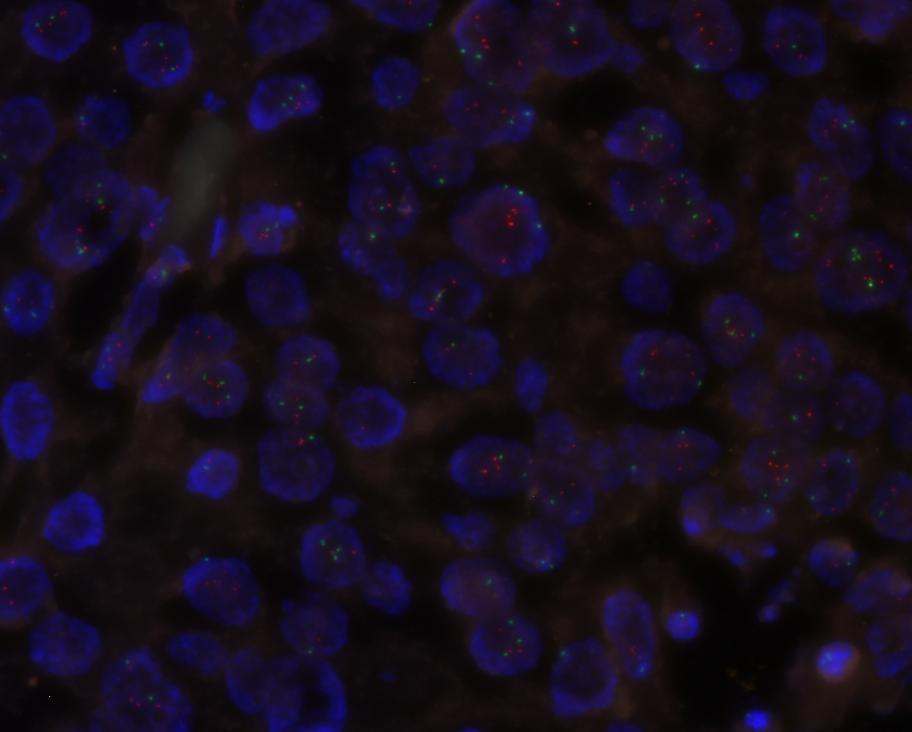
\includegraphics[width=6.0cm,height=6.0cm]{images/Her2Fish/her21.jpg}
%
%By projecting out the luminance information, an initial
%segmentation can be obtained by clustering in chromaticity
%space.
%
%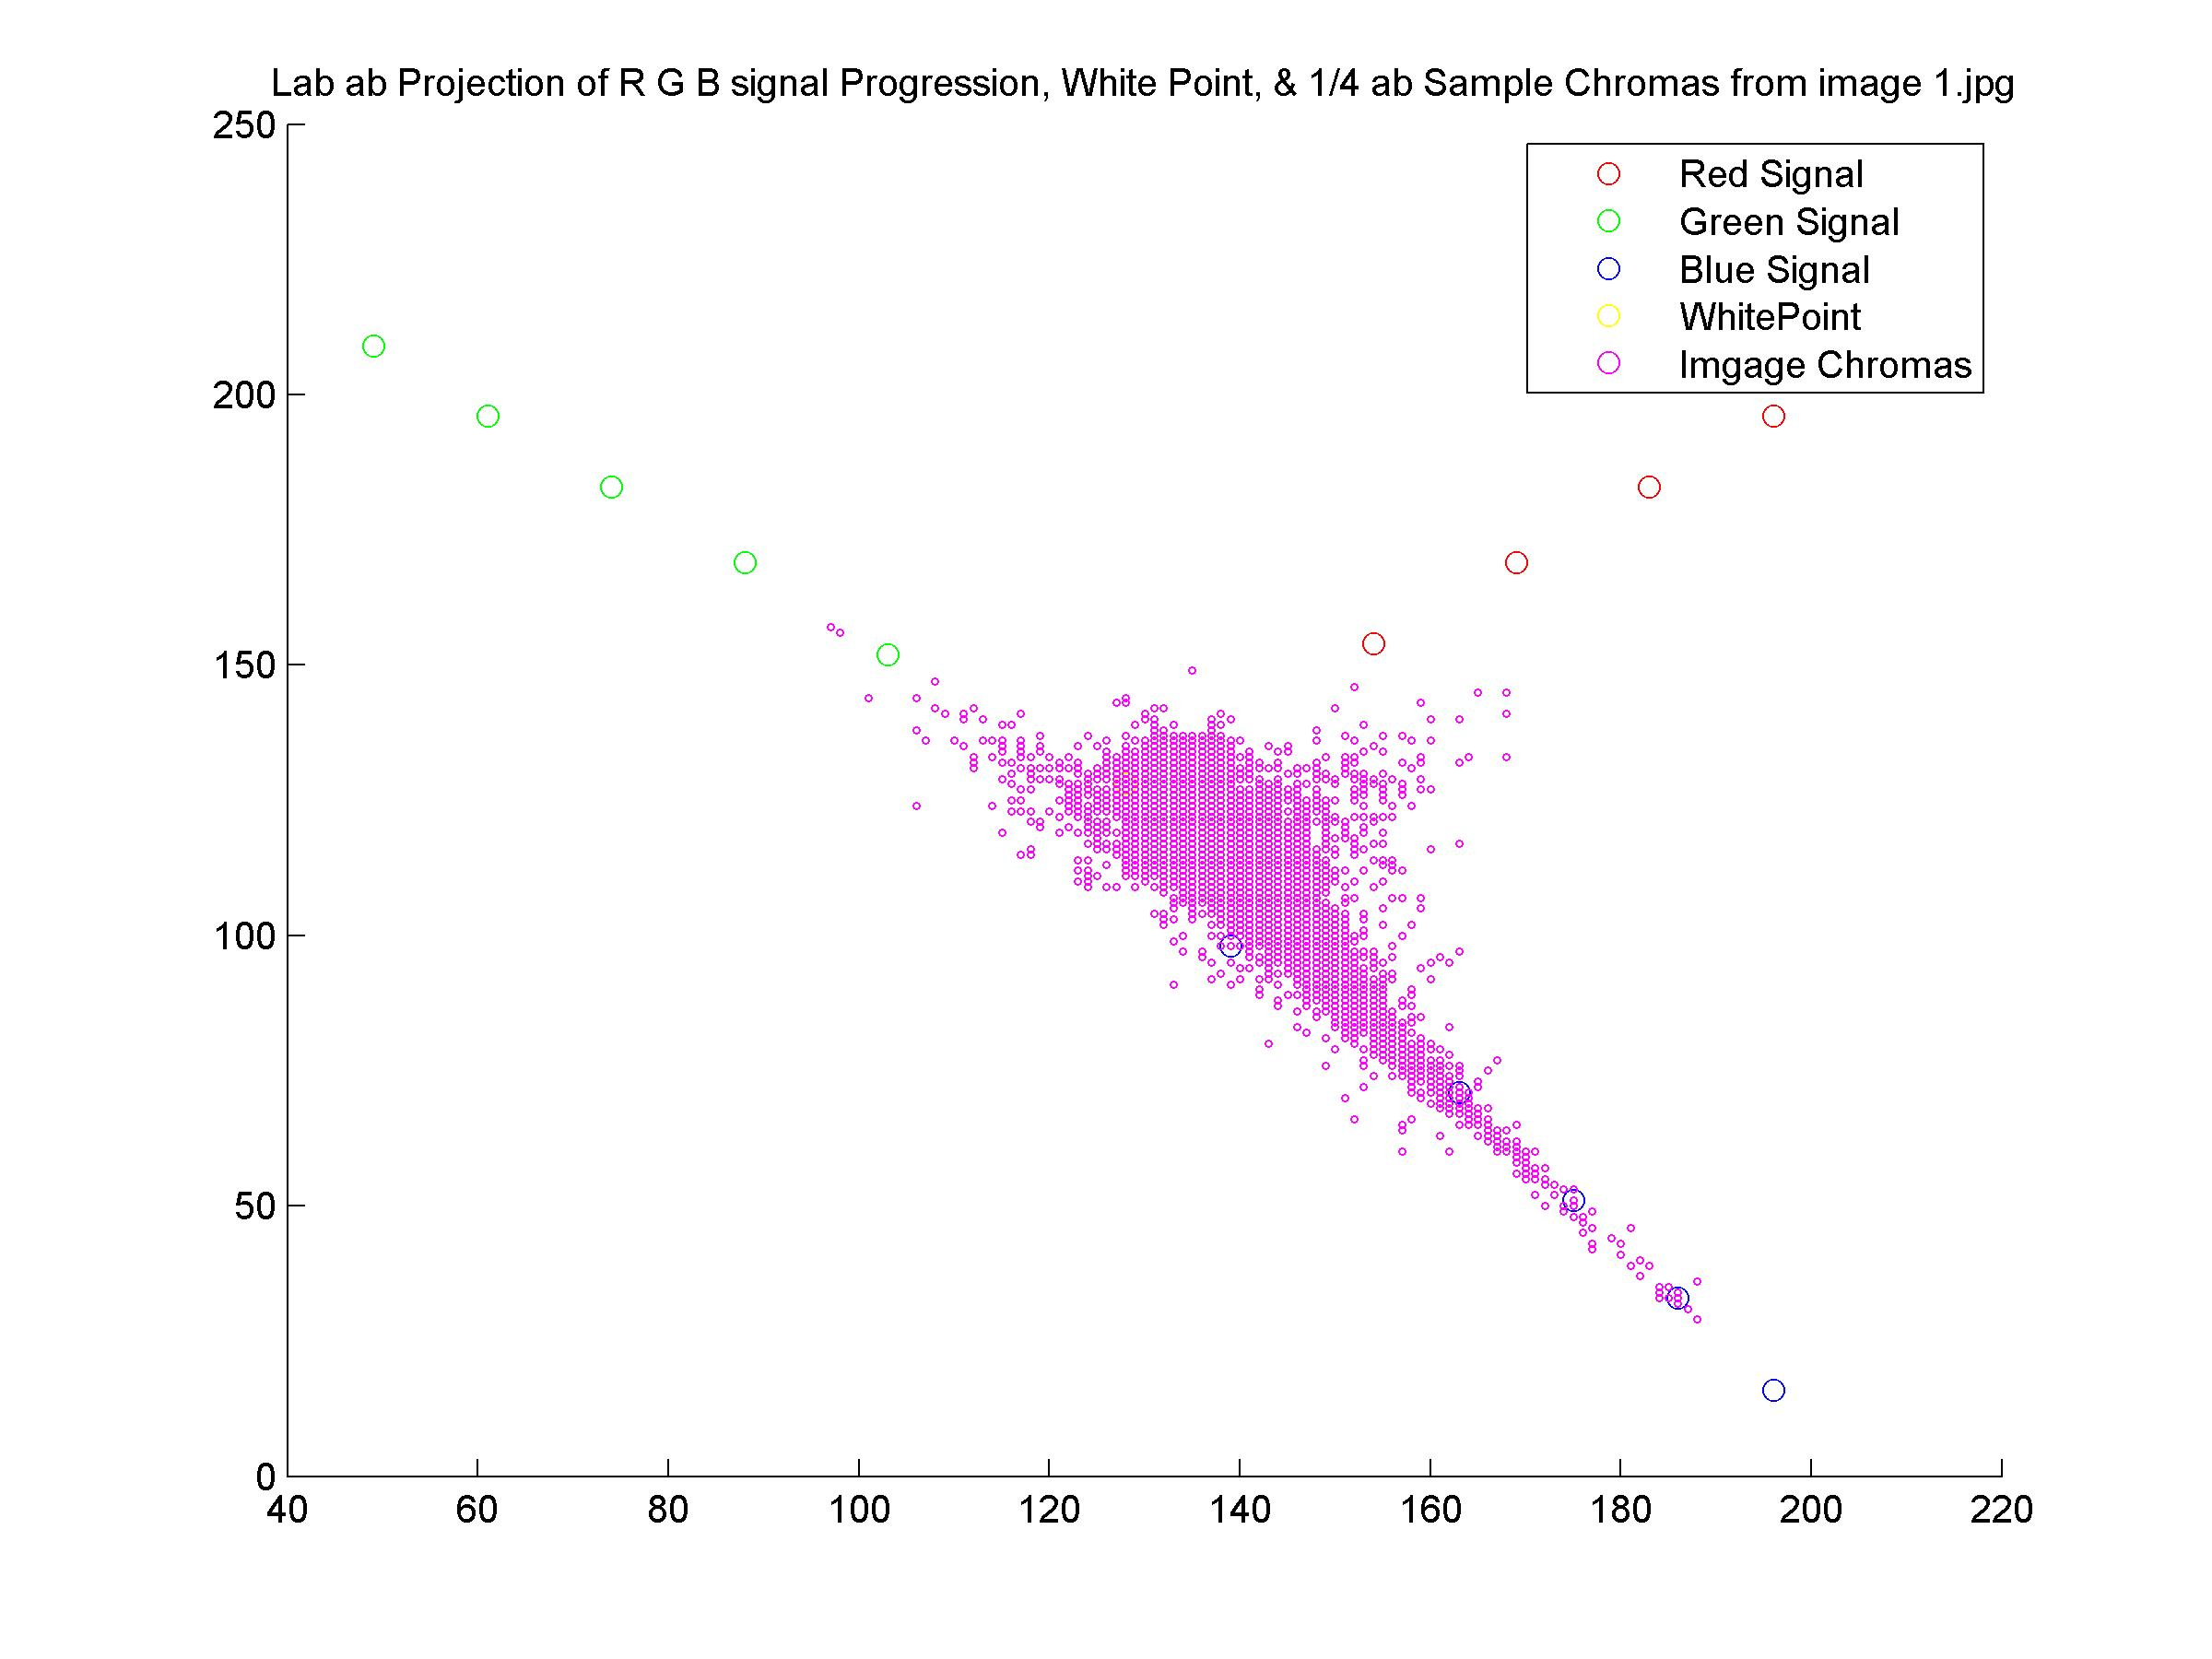
\includegraphics[width=6.0cm,height=6.0cm]{images/Her2Fish/1_SampleChromas.jpg}
%
%
%Using 6 seed points, a k-means segmentation was produced.
%
%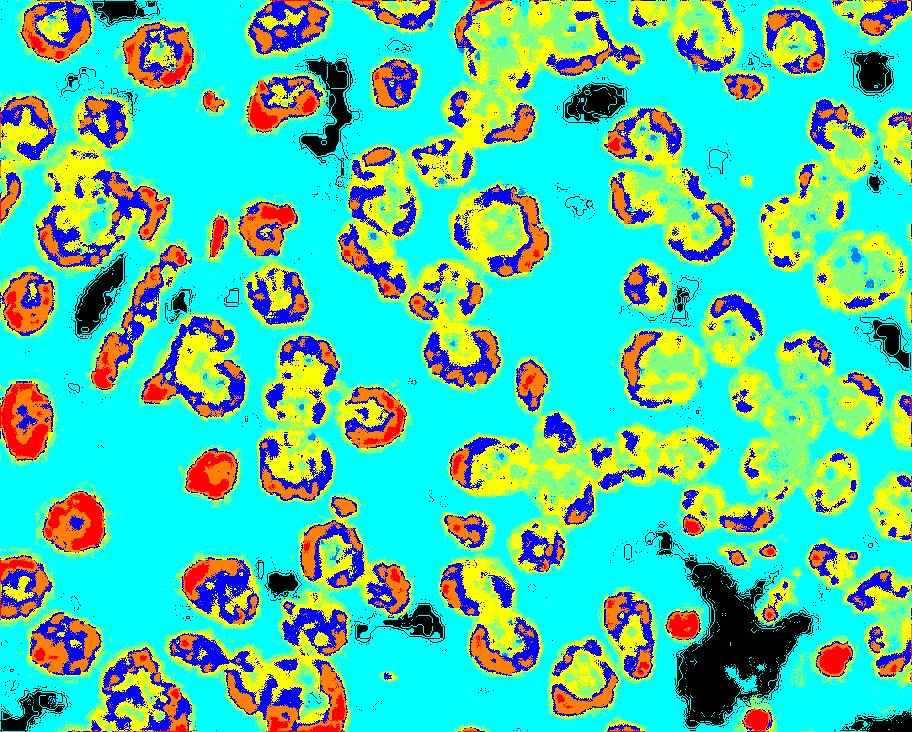
\includegraphics[width=6.0cm,height=6.0cm]{images/Her2Fish/1_RGB_LabelImg.jpg}
%
%Notice not all of the cells are well separated. A watershed
%transform uses spatial clustering to segment overlapping cells.
%
%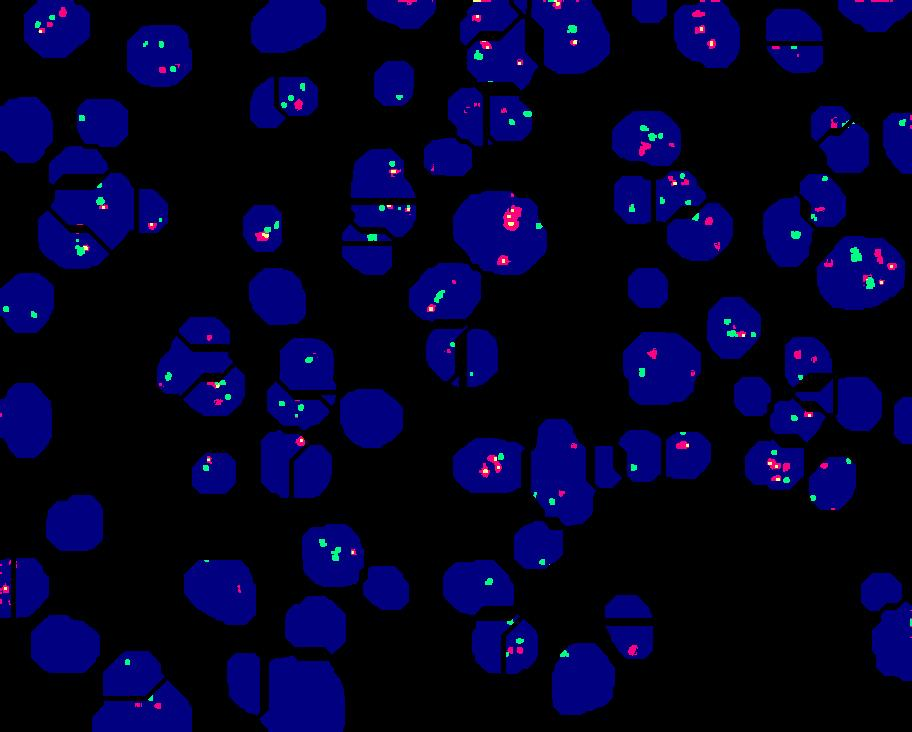
\includegraphics[width=6.0cm,height=6.0cm]{images/Her2Fish/1_RGBMASK.jpg}
%

\section{Machine Vision Techniques in Automated Pathology}

%MachineVision_Pathology_ExampleSlides_Page_03.jpg
%MachineVision_Pathology_ExampleSlides_Page_05.jpg
%MachineVision_Pathology_ExampleSlides_Page_06.jpg
%MachineVision_Pathology_ExampleSlides_Page_07.jpg
%MachineVision_Pathology_ExampleSlides_Page_08.jpg
%MachineVision_Pathology_ExampleSlides_Page_09.jpg
%MachineVision_Pathology_ExampleSlides_Page_11.jpg
%MachineVision_Pathology_ExampleSlides_Page_13.jpg
%MachineVision_Pathology_ExampleSlides_Page_15.jpg
%MachineVision_Pathology_ExampleSlides_Page_16.jpg
A small subset of features and samples from development efforts to automatically detect hepatic hypertrophy in rat. This is an example of quantitative tissue analysis on 2GB H\&E rat liver images scanned at 0.5 micron. Each pixel on the heat map corresponds to a 1024x1024 image tile. Each tile was segmented into several thousand objects in one or more of 10
biologically meaningful classes. Models for scoring tiles were fit to overall path grades and to an intergrade ordinal model based on expert comparative vision experiments. This study consisted of 5TB of highly variable image data. A magnification of 200\% is recommended for viewing the heat maps
\begin{tabular}{ |c|c| }
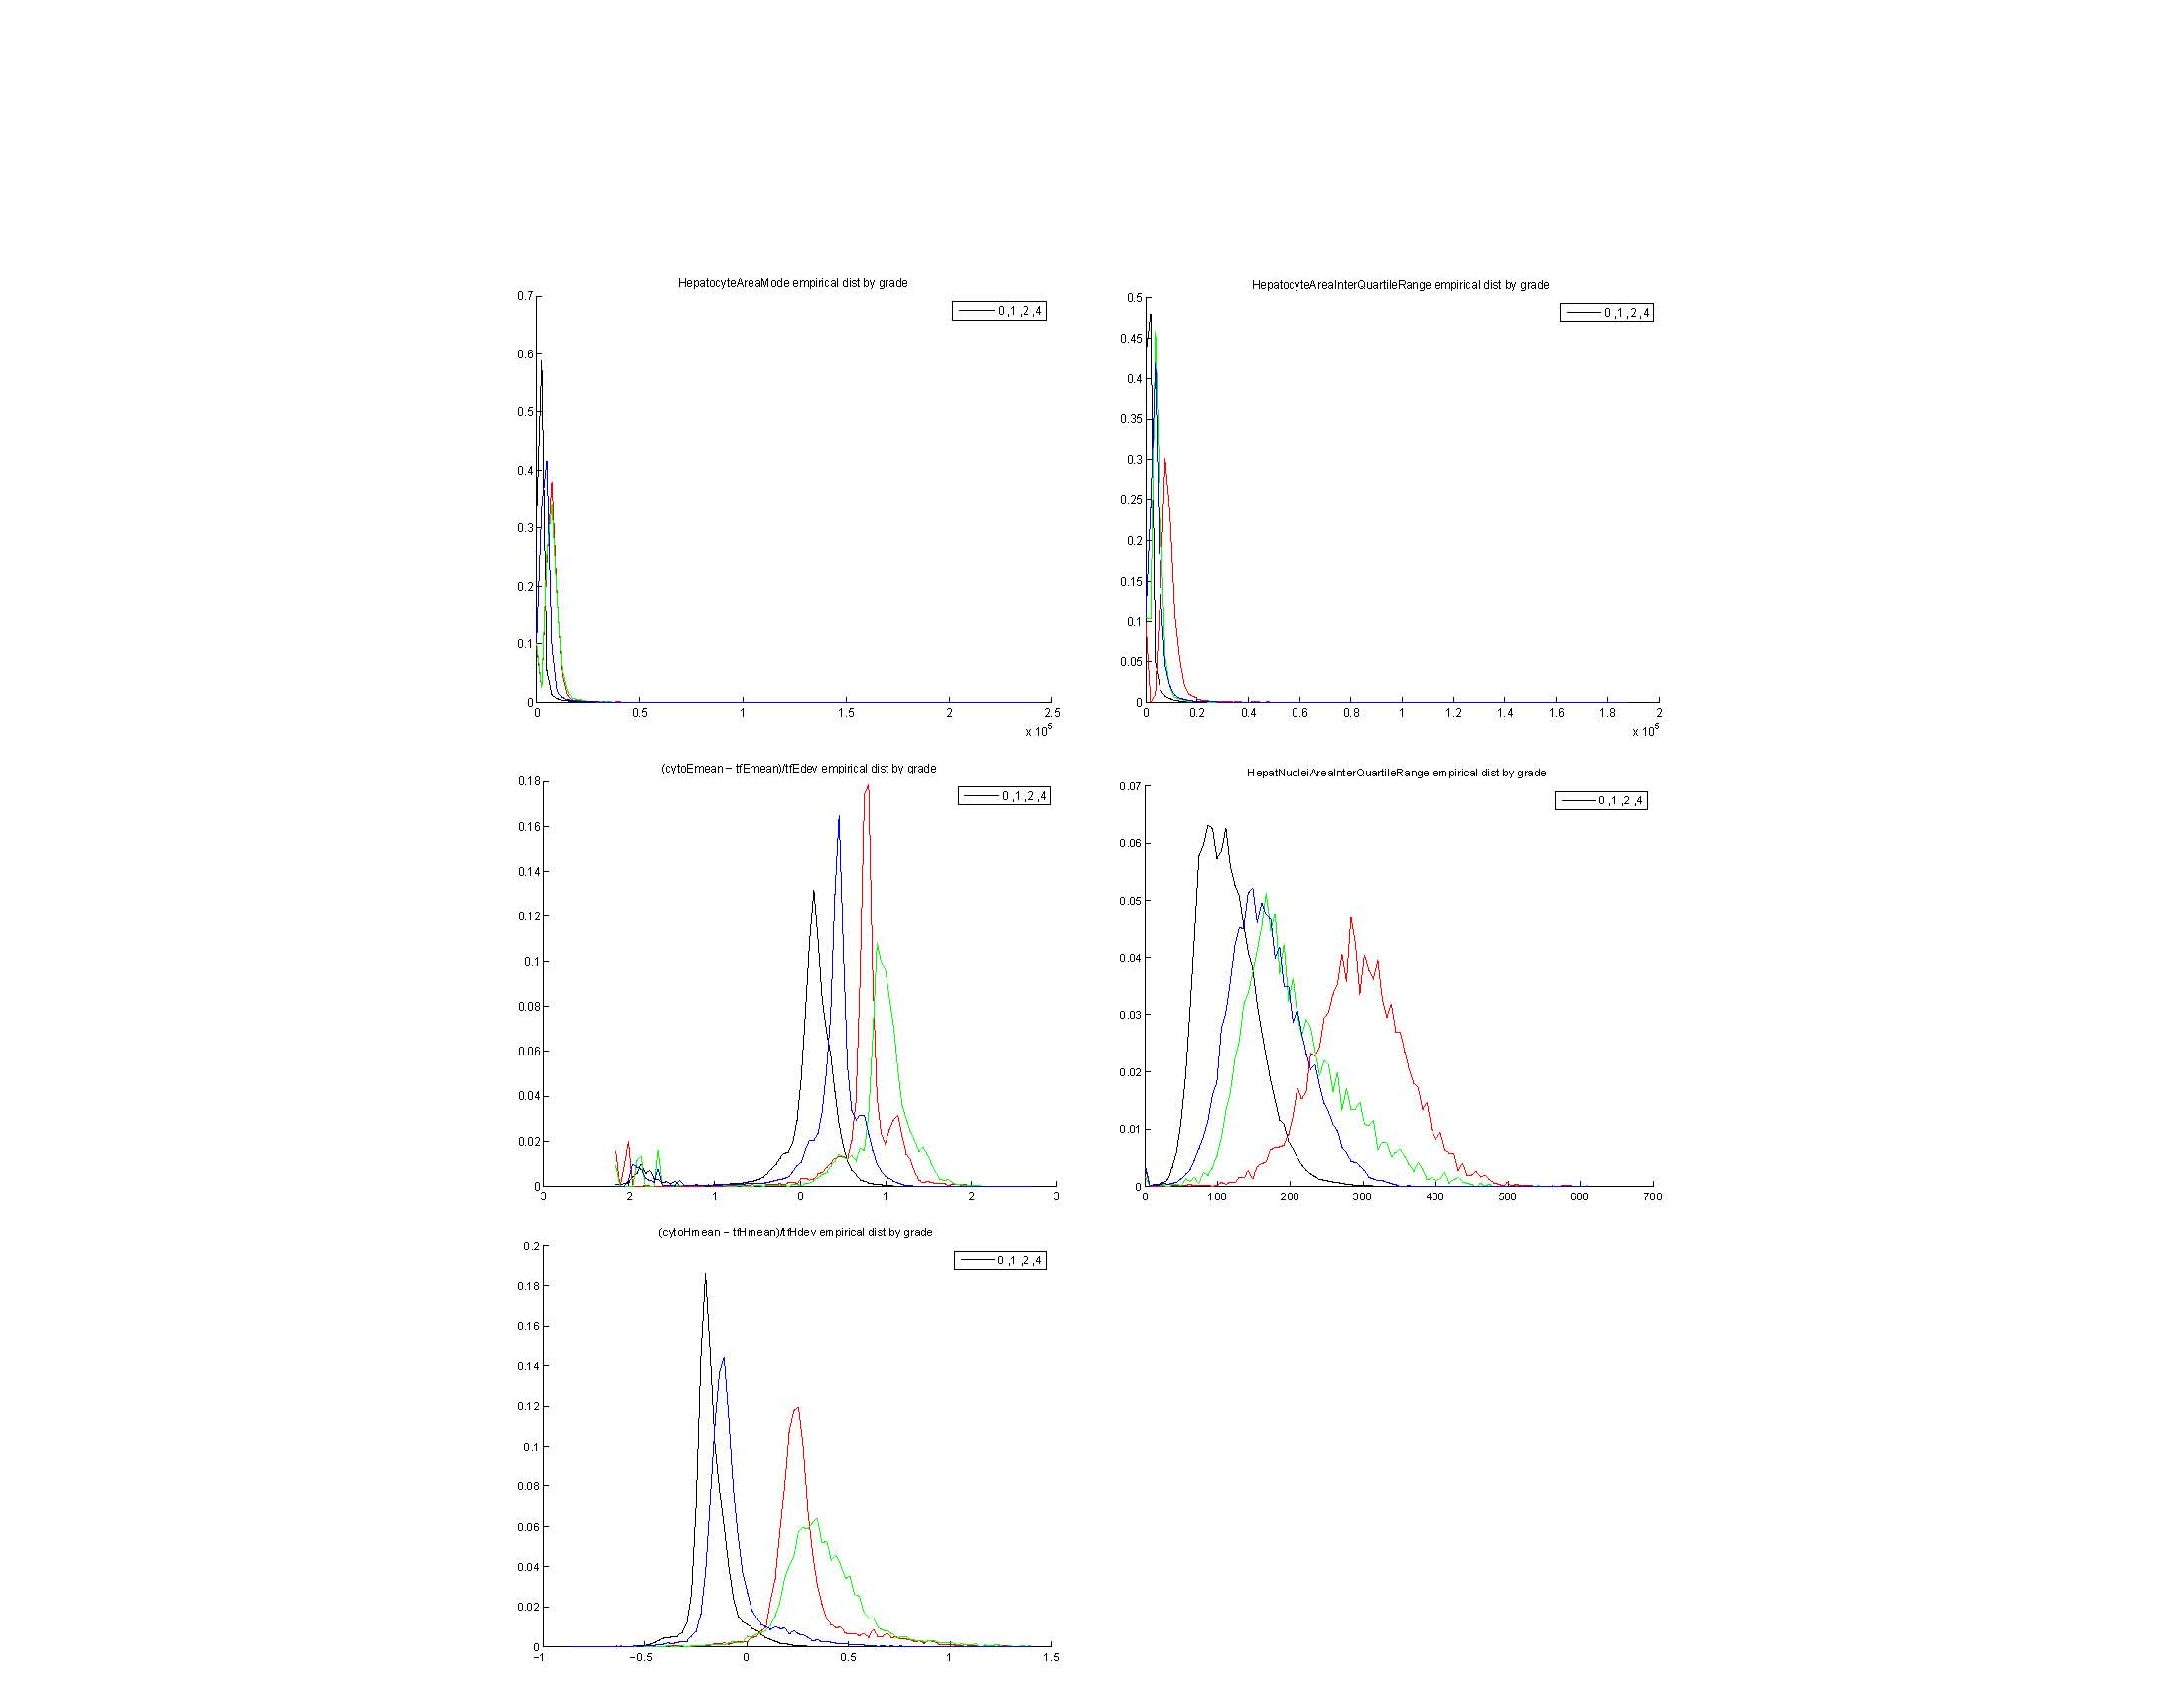
\includegraphics[width=4.0cm,height=4.0cm]{images/MachineVision/MachineVision_Pathology_ExampleSlides_Page_03.jpg} &
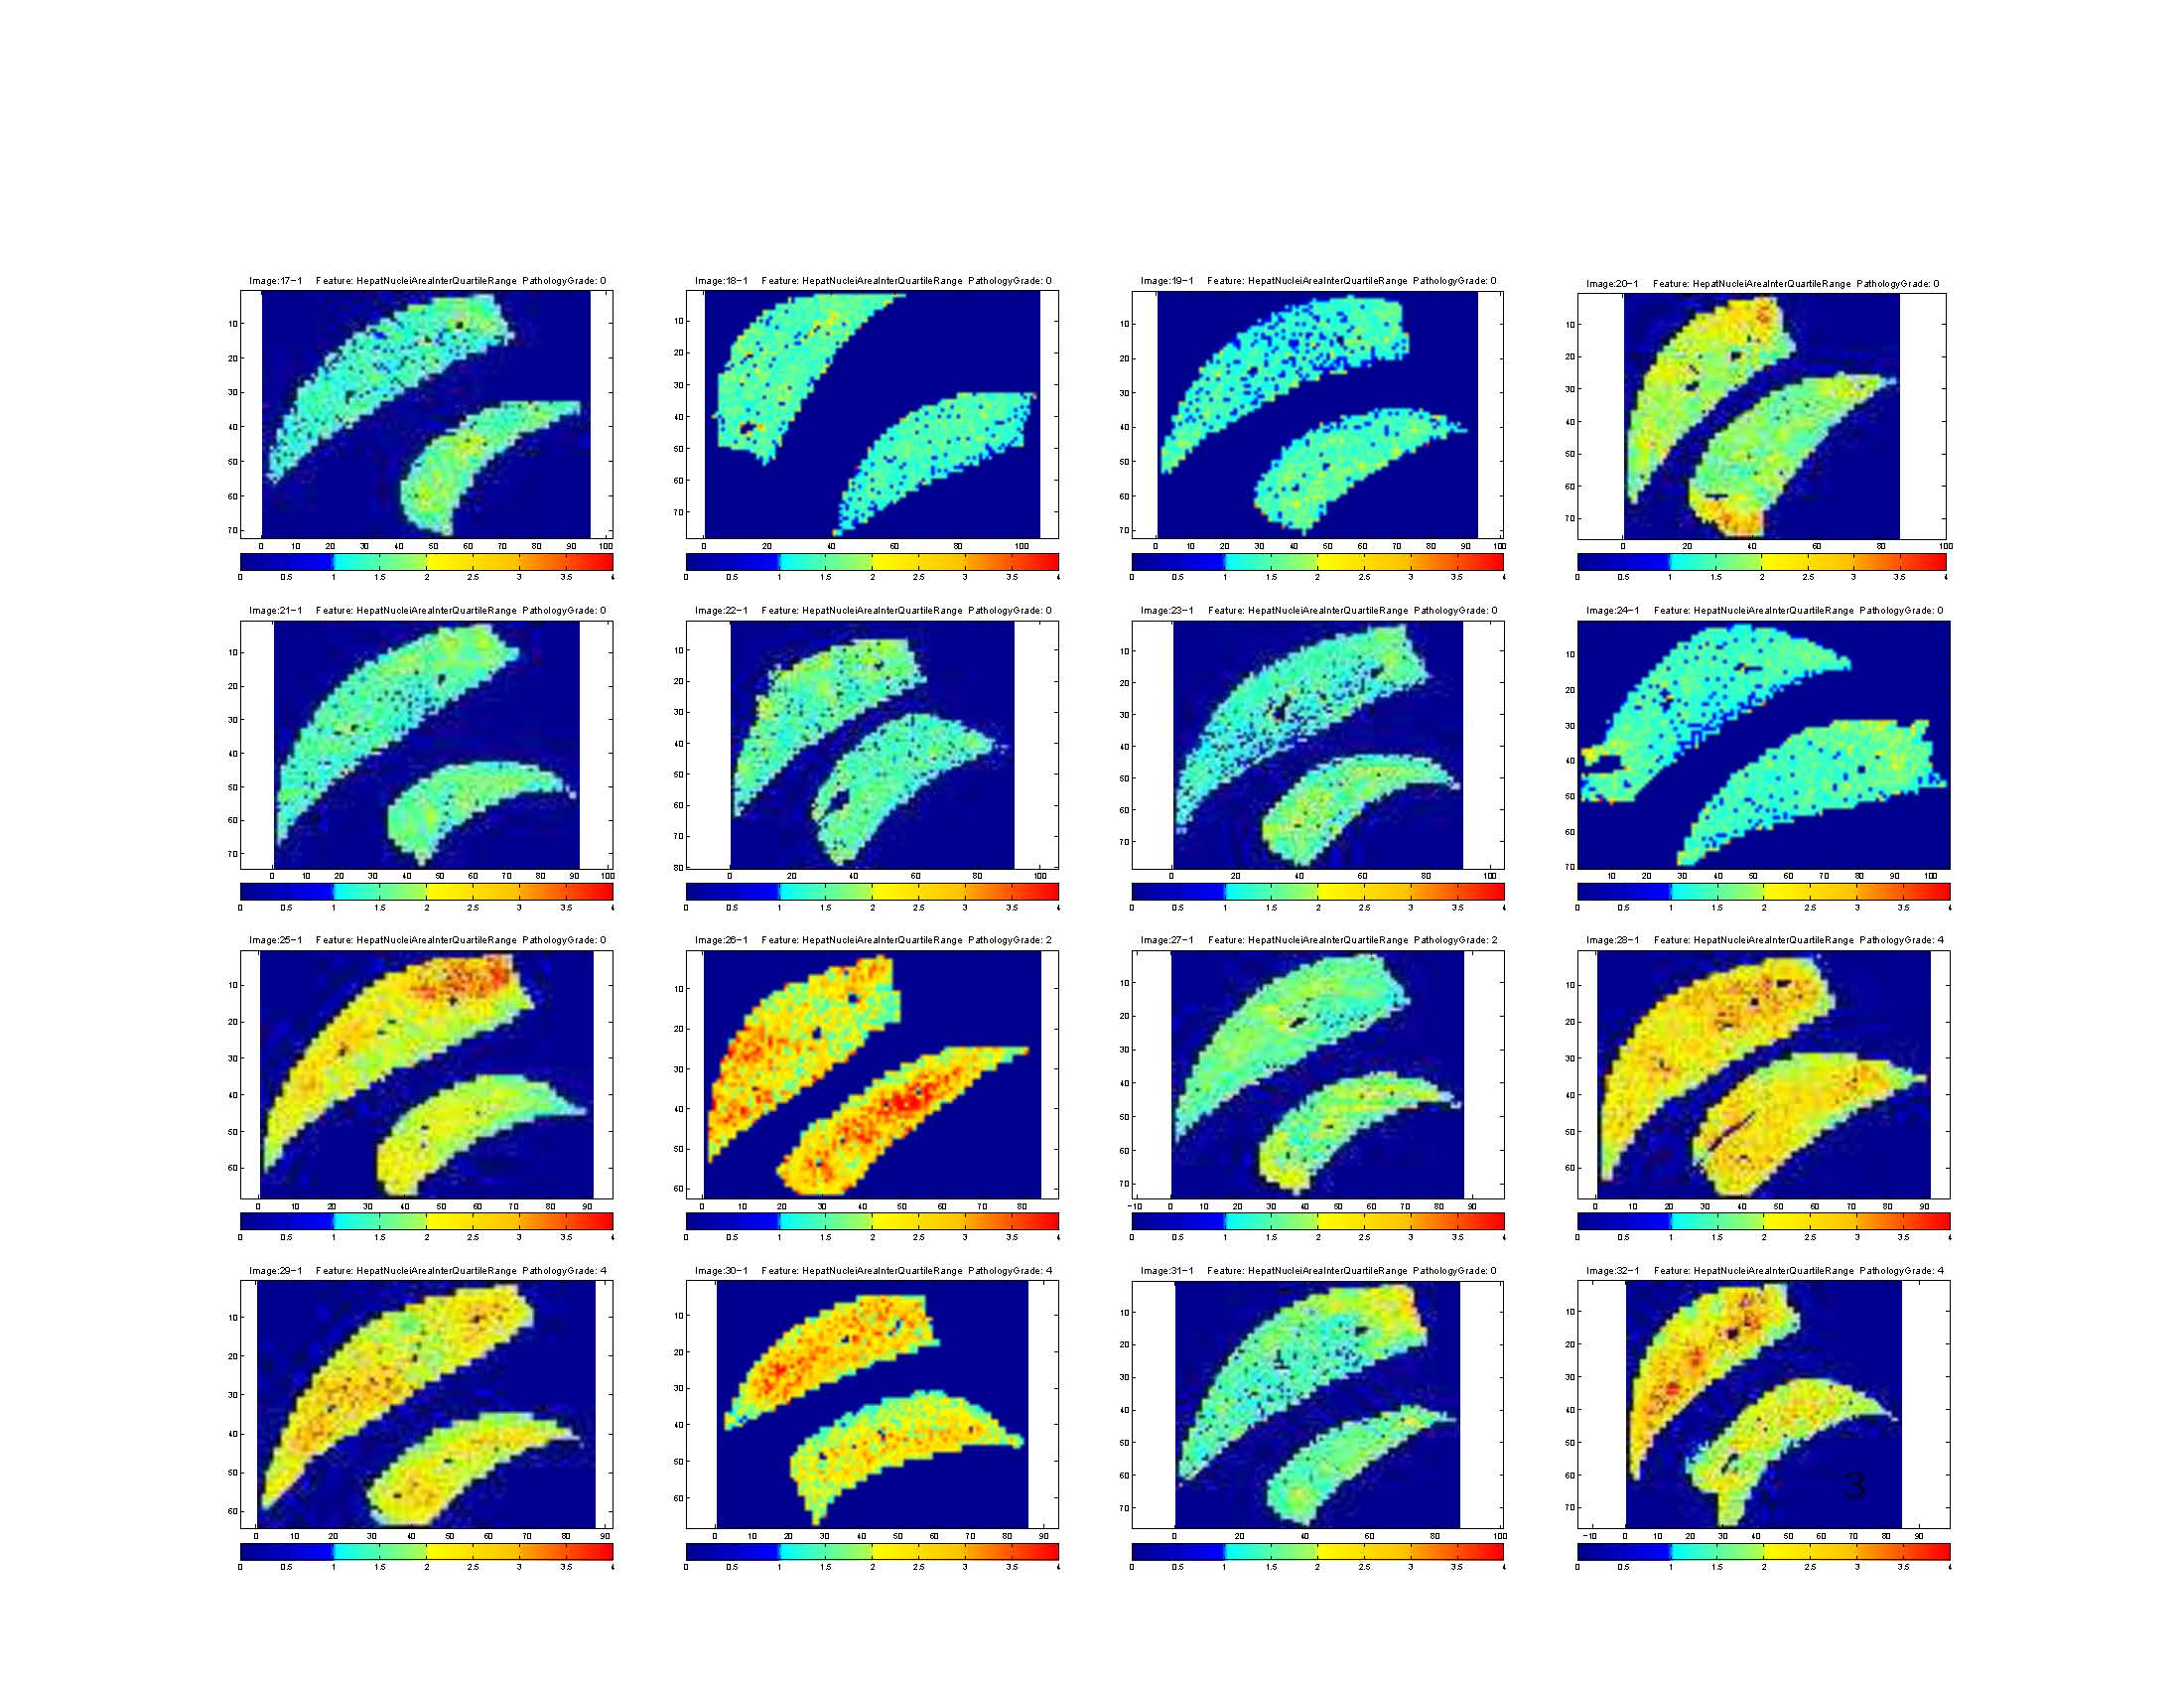
\includegraphics[width=4.0cm,height=4.0cm]{images/MachineVision/MachineVision_Pathology_ExampleSlides_Page_05.jpg} \\
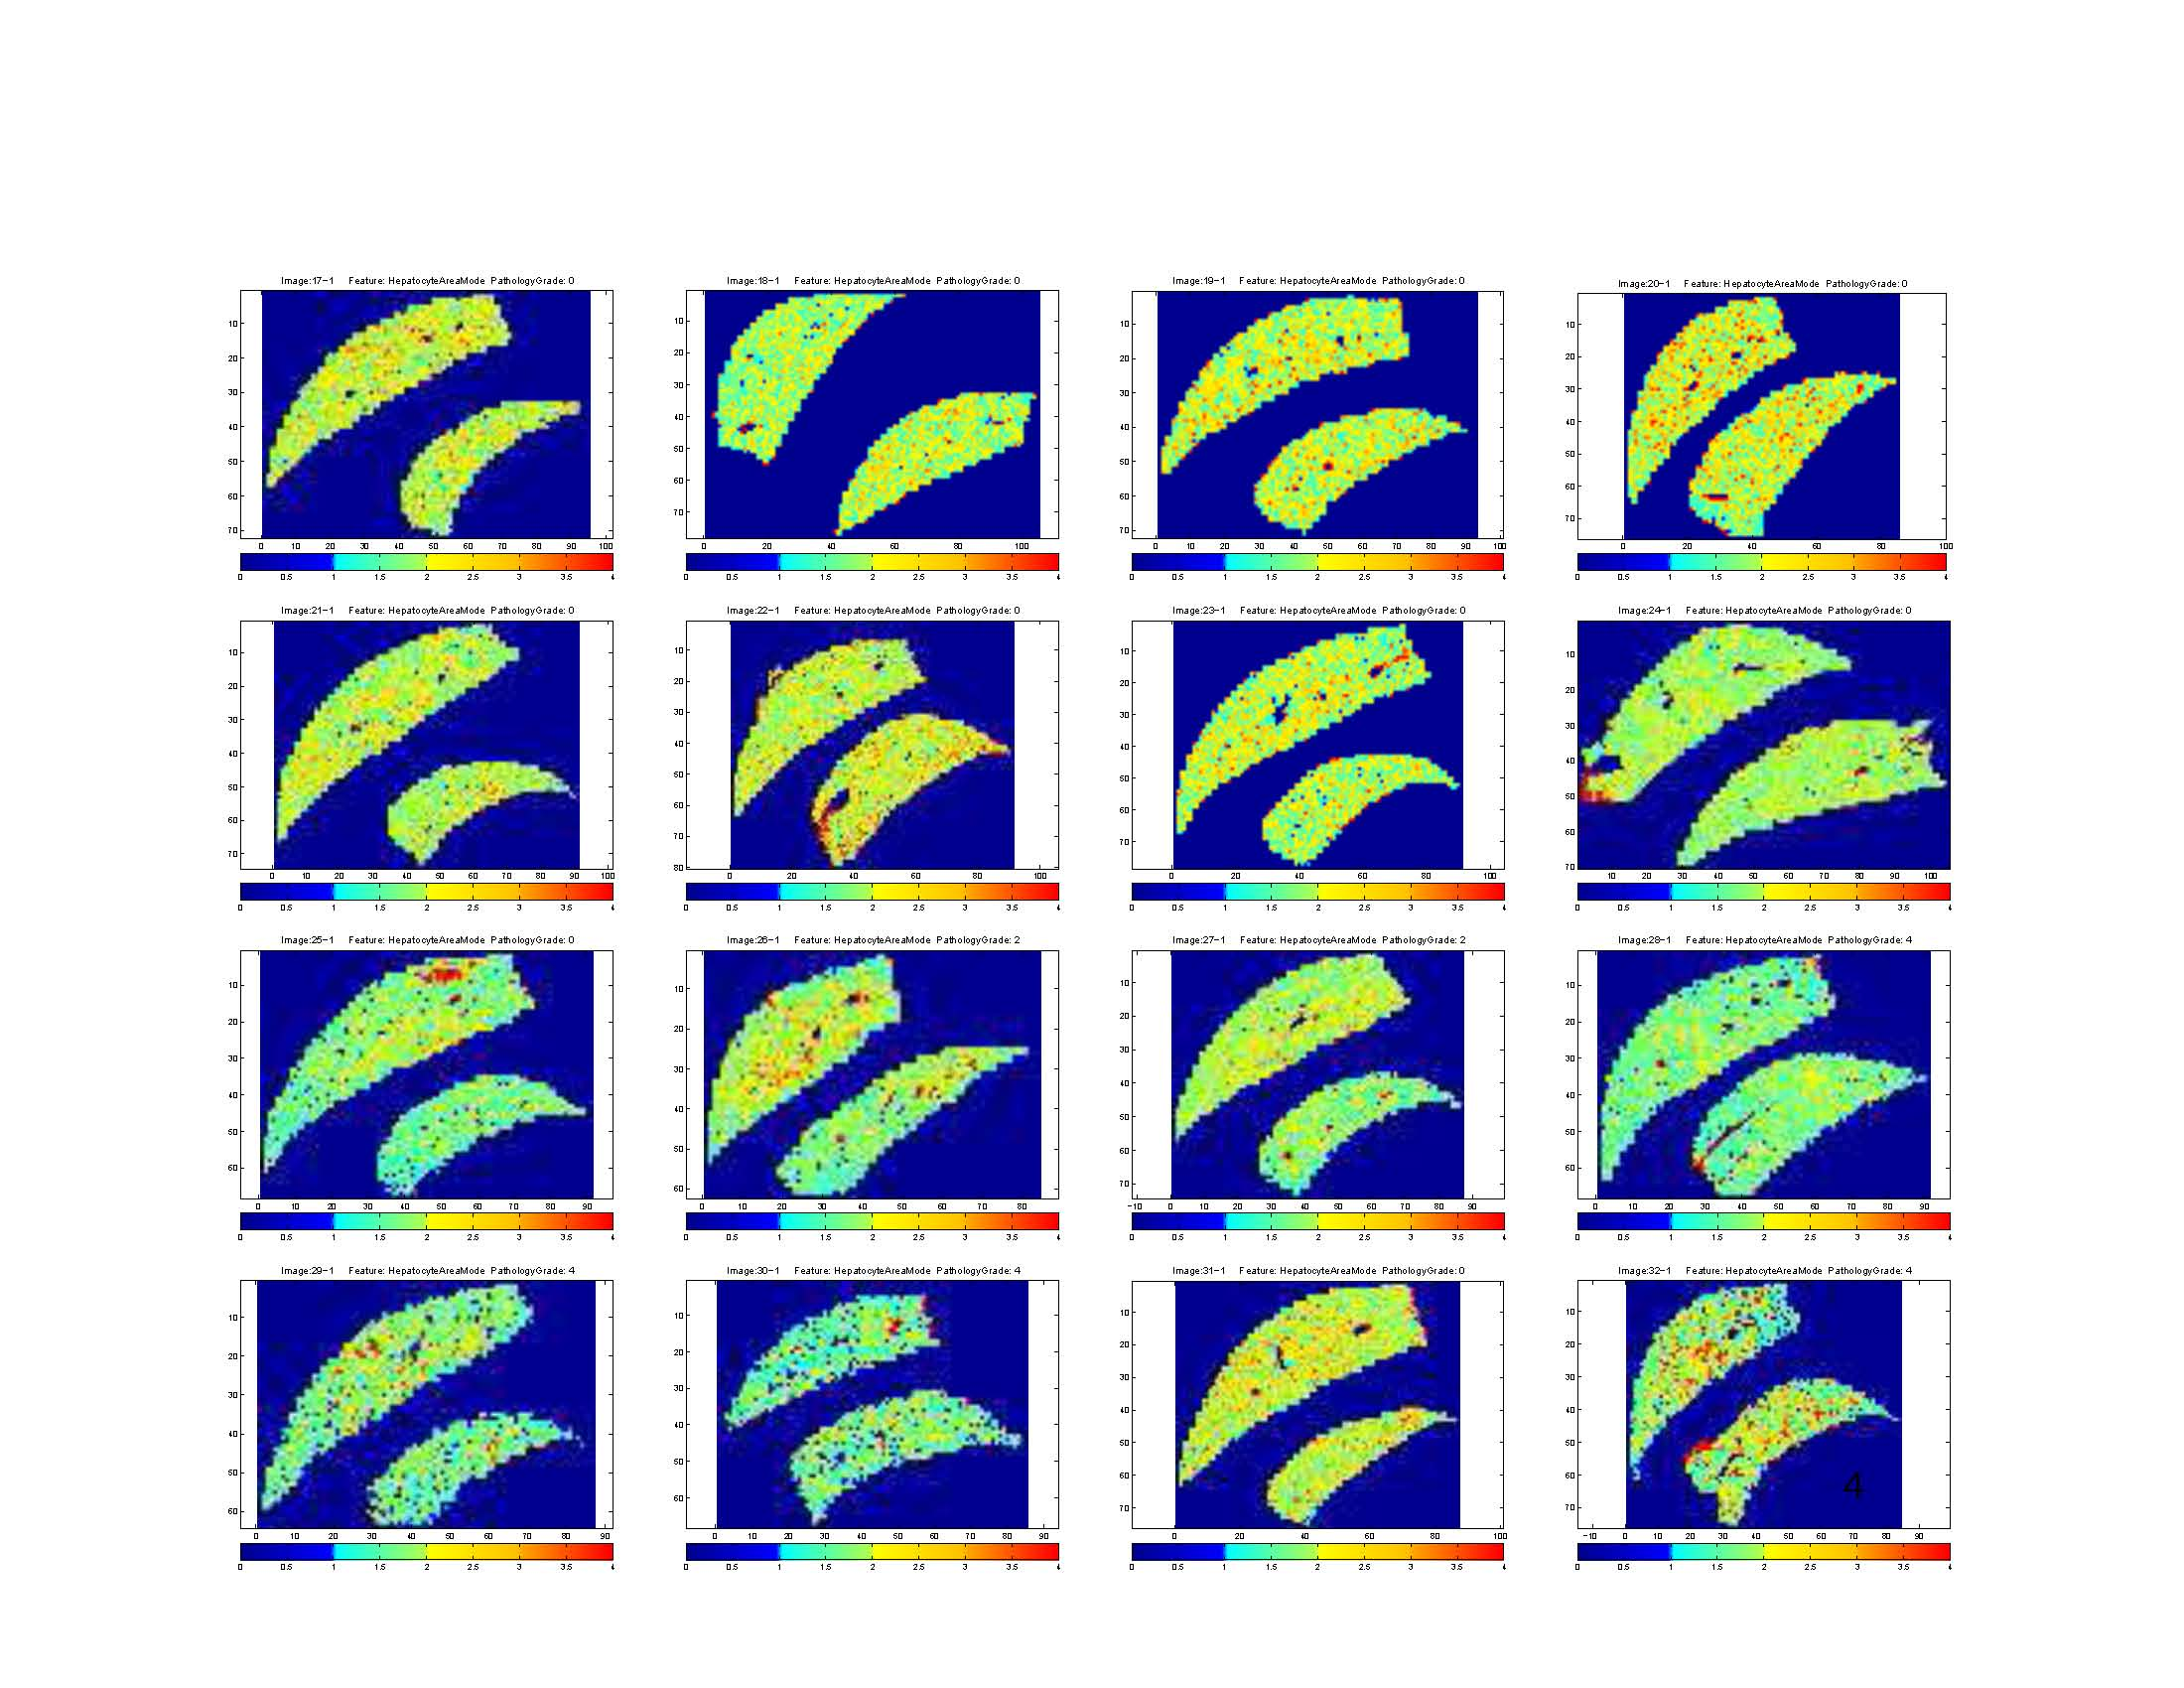
\includegraphics[width=4.0cm,height=4.0cm]{images/MachineVision/MachineVision_Pathology_ExampleSlides_Page_06.jpg} &
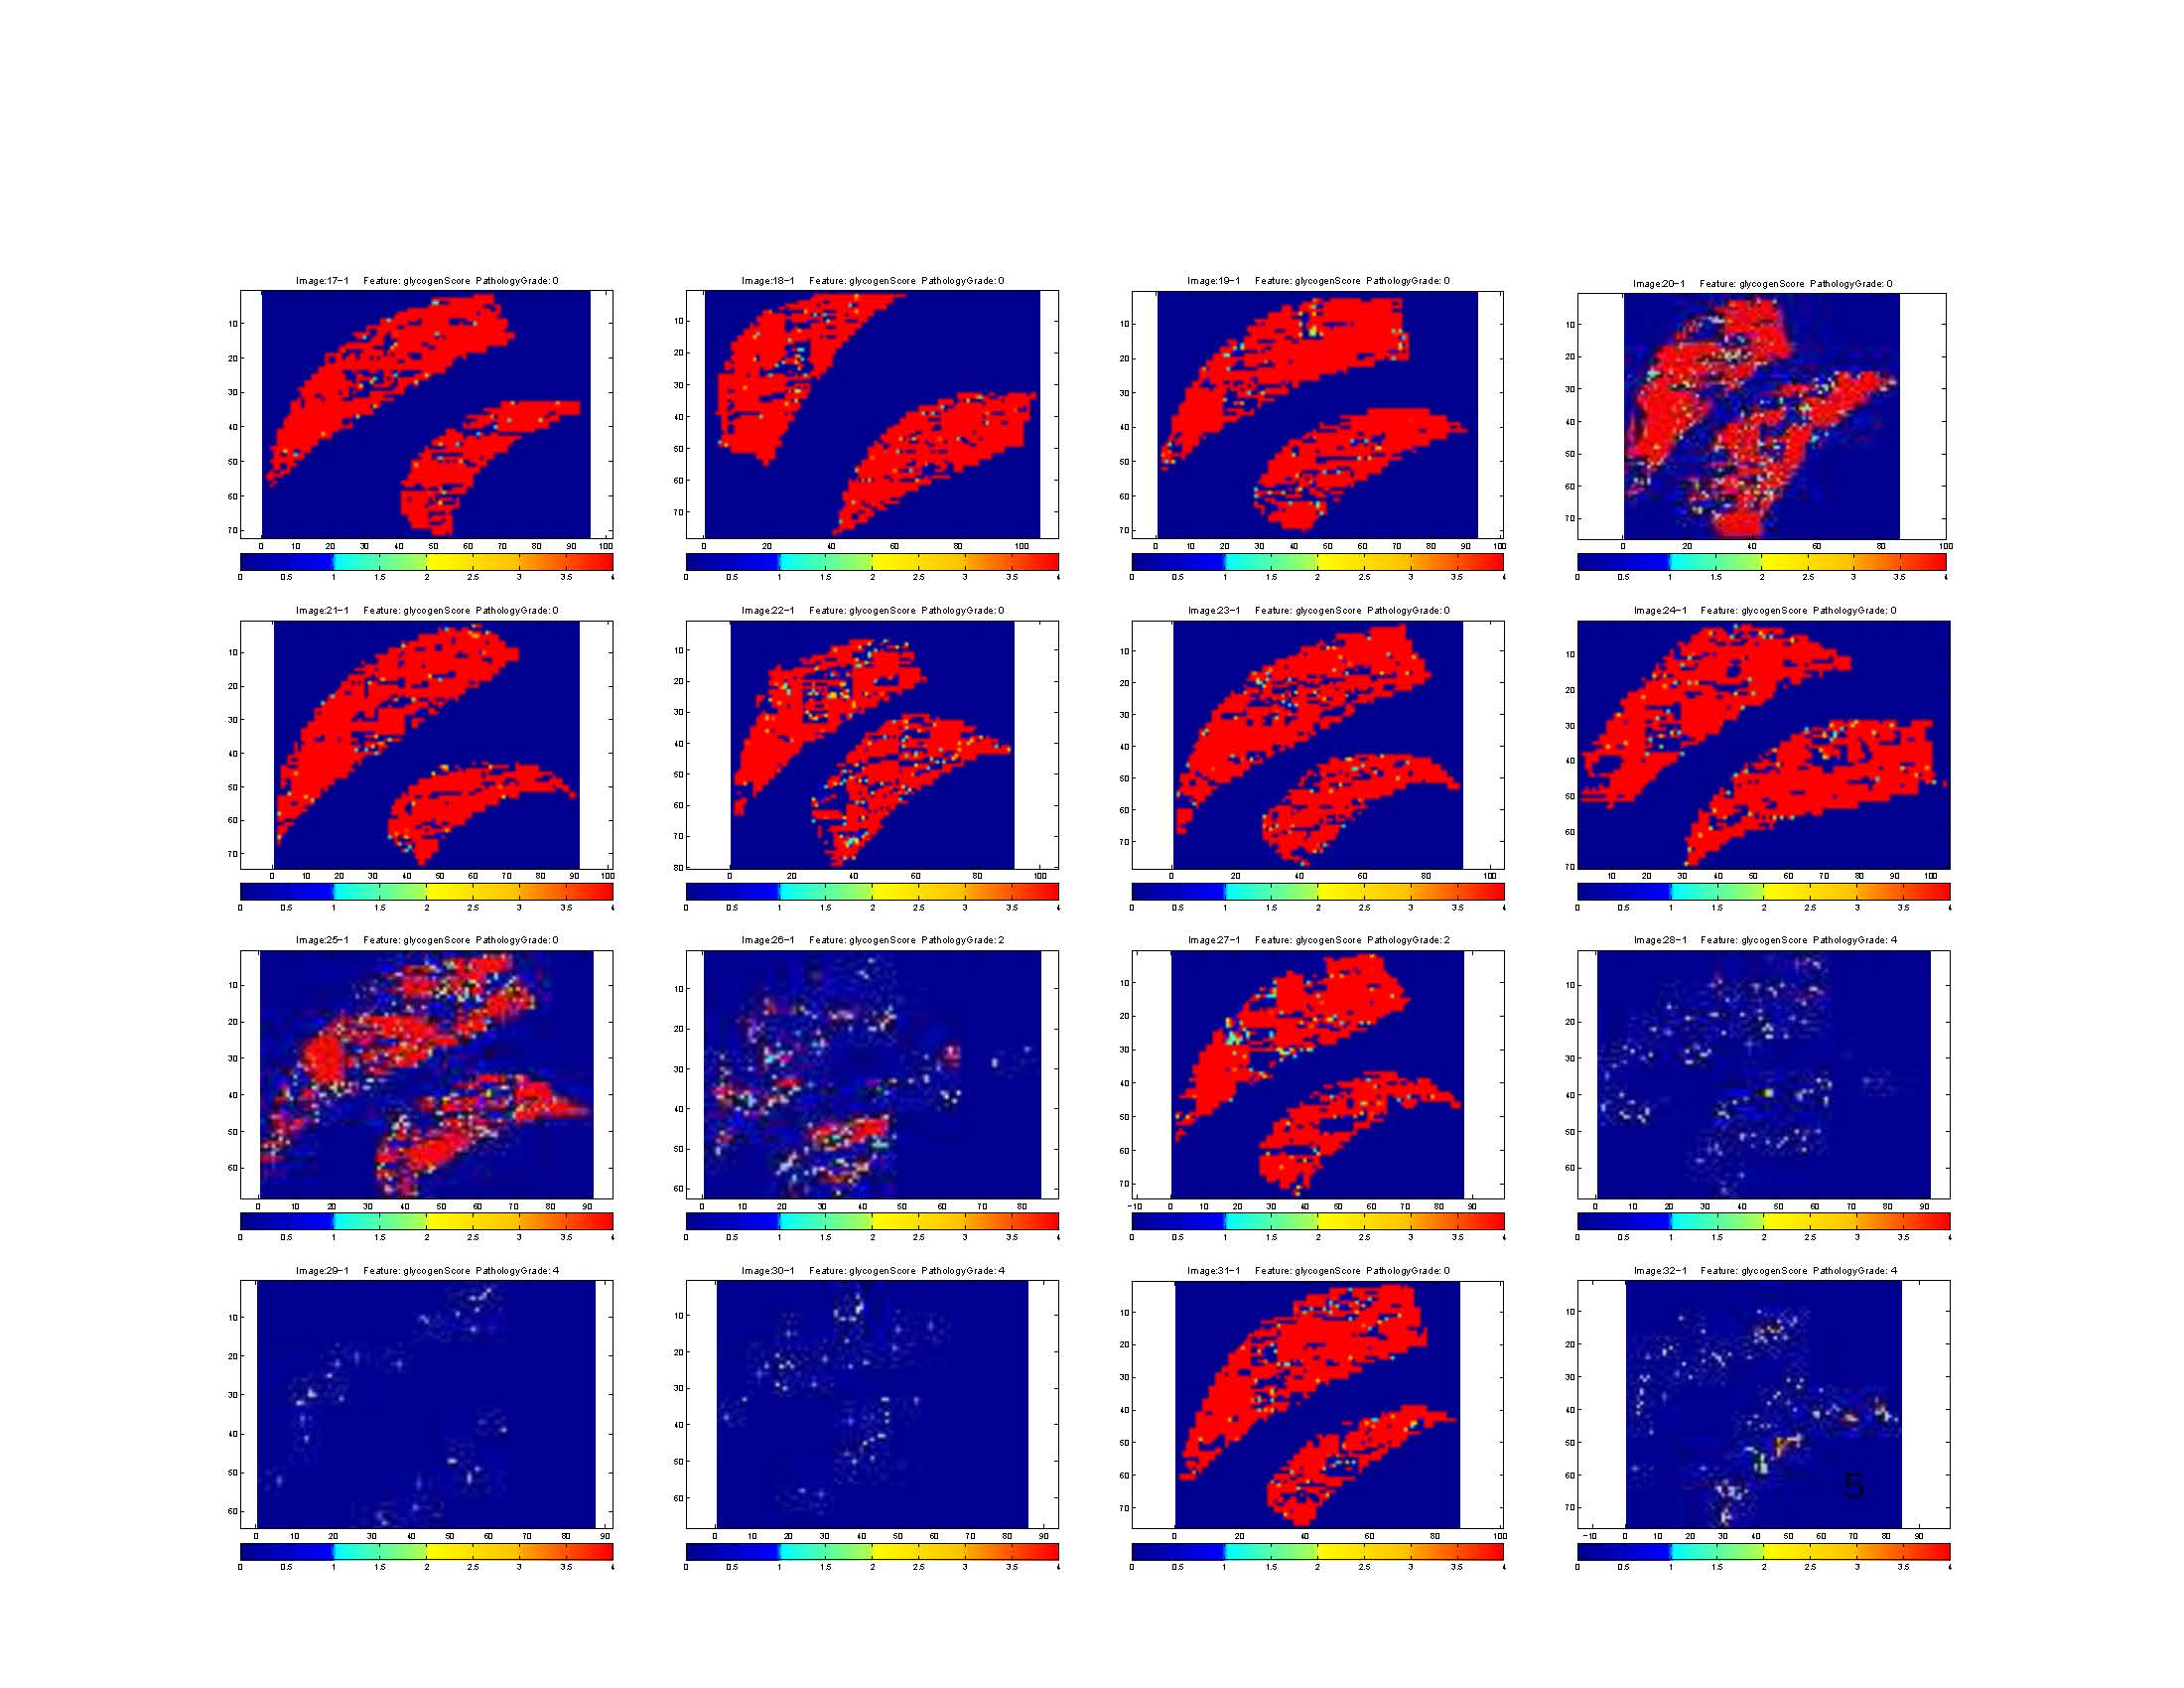
\includegraphics[width=4.0cm,height=4.0cm]{images/MachineVision/MachineVision_Pathology_ExampleSlides_Page_07.jpg} \\
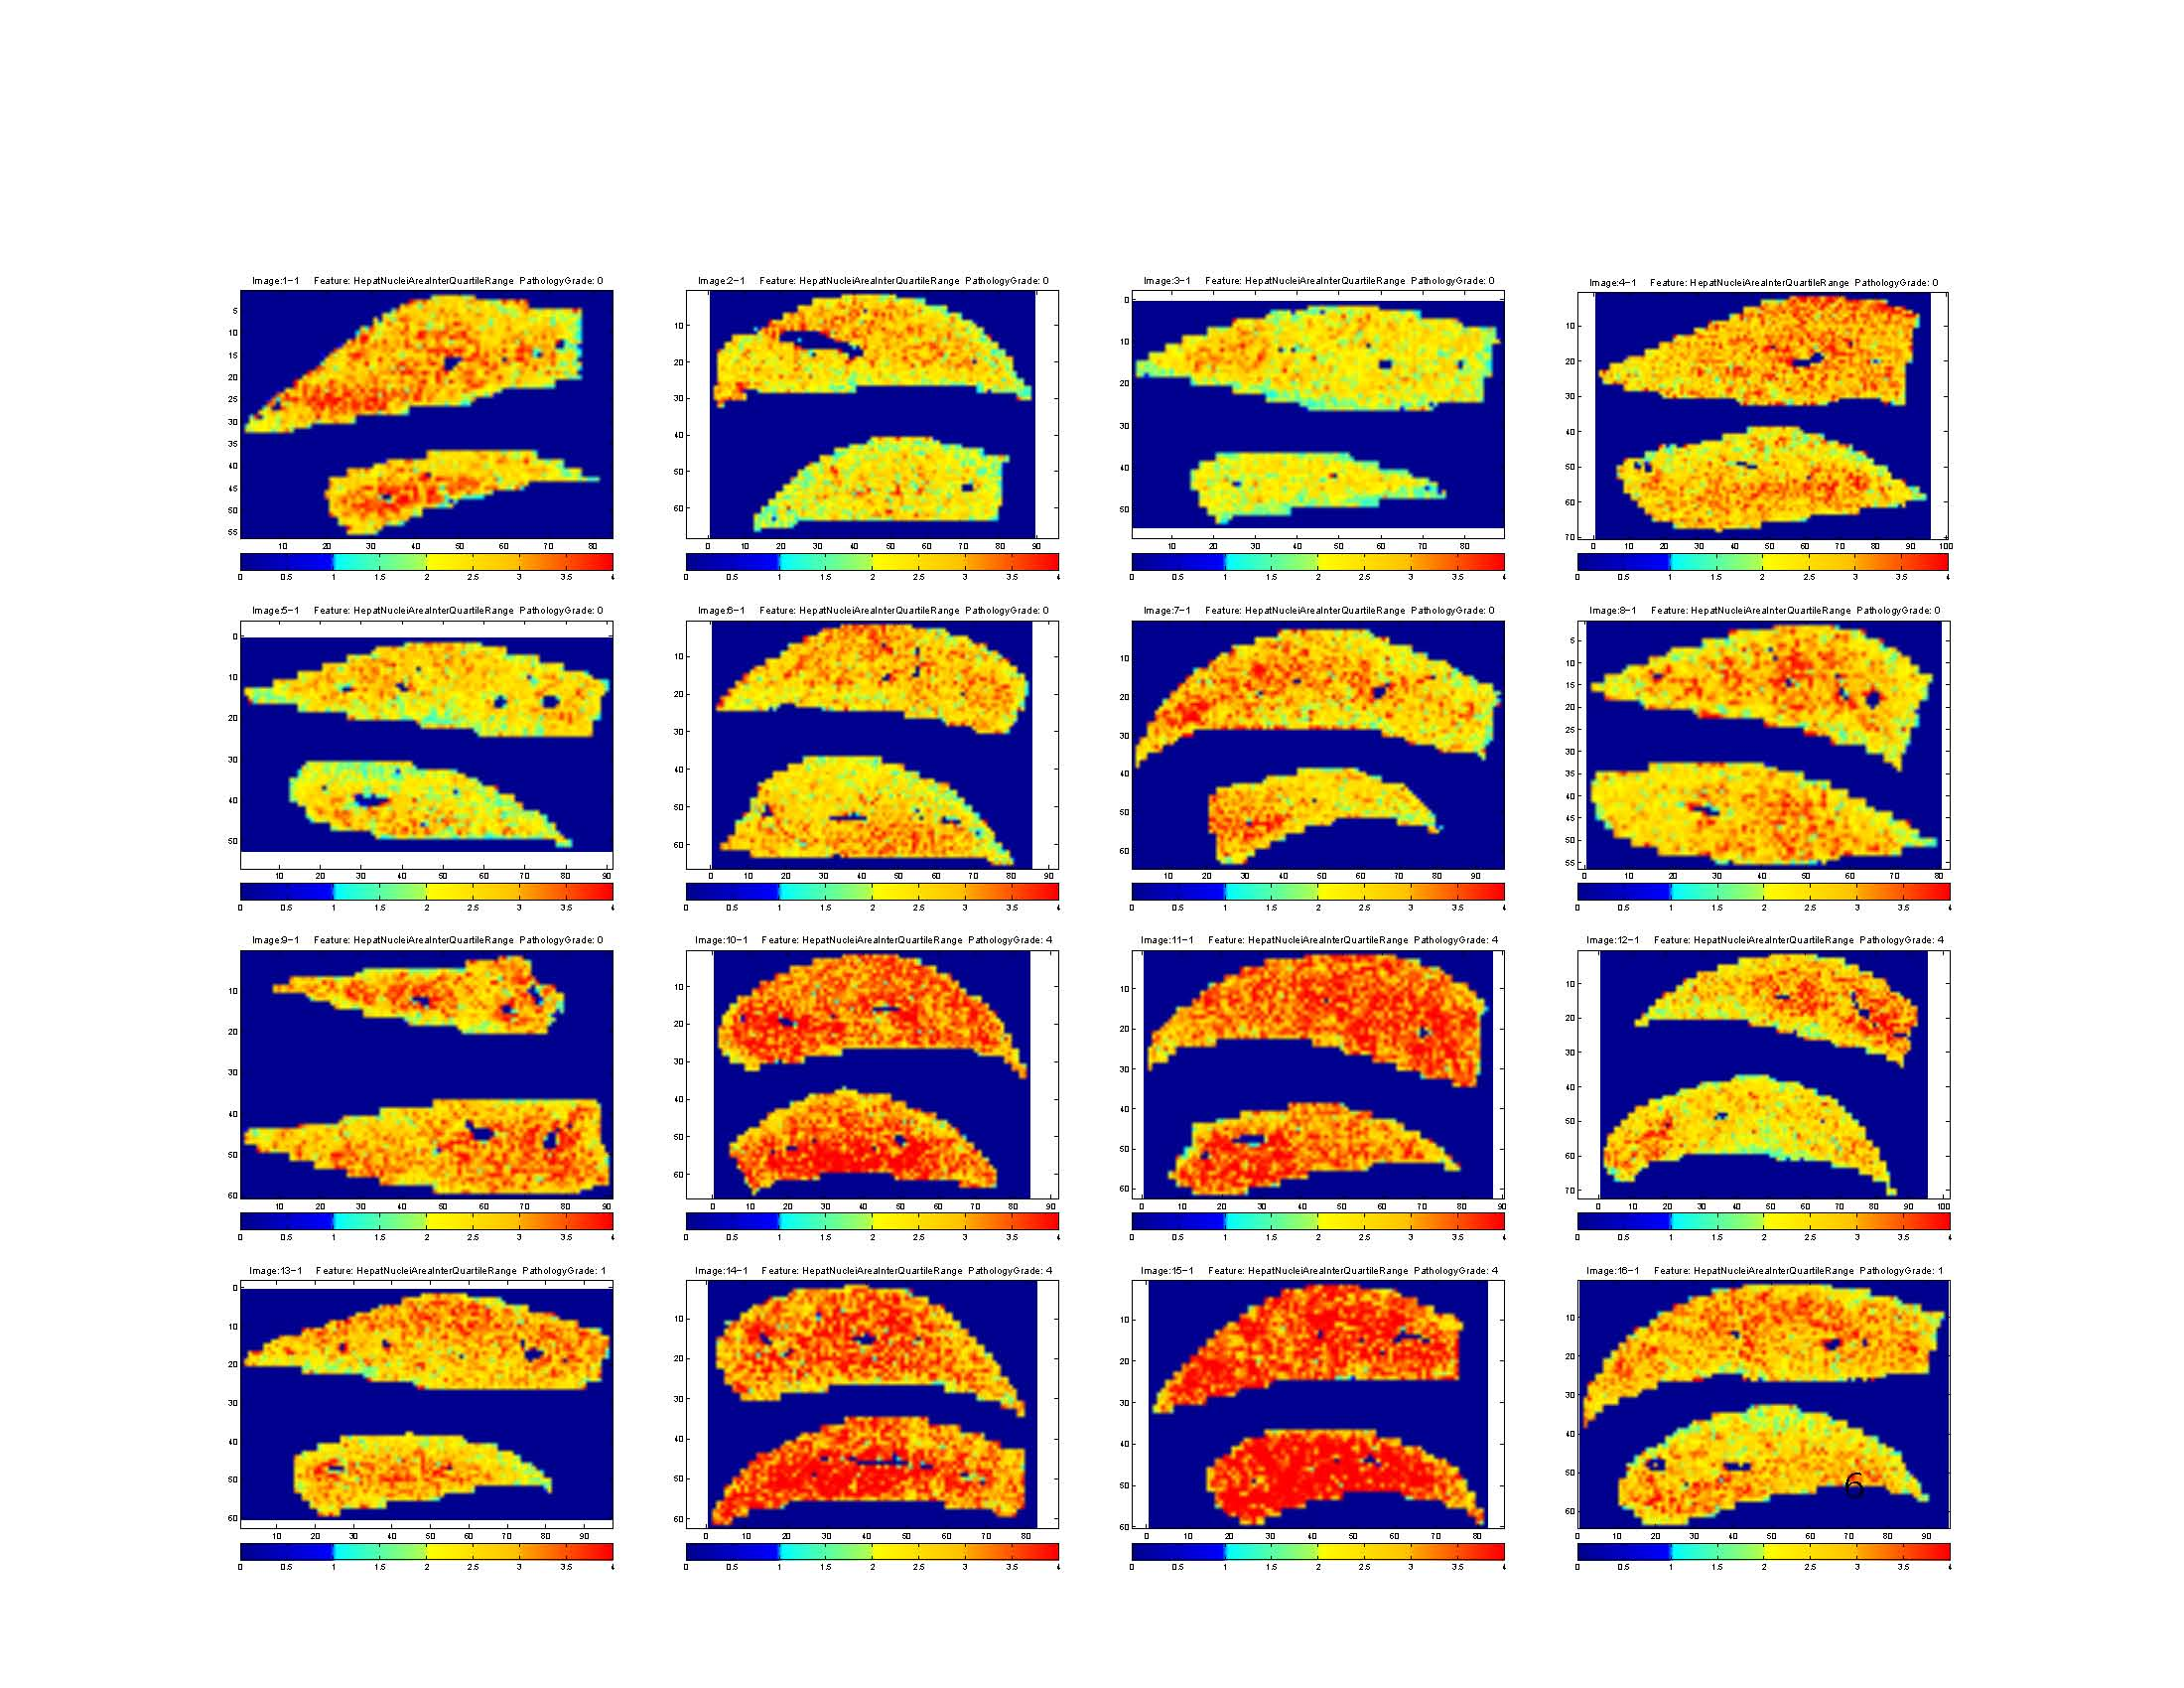
\includegraphics[width=4.0cm,height=4.0cm]{images/MachineVision/MachineVision_Pathology_ExampleSlides_Page_08.jpg} &
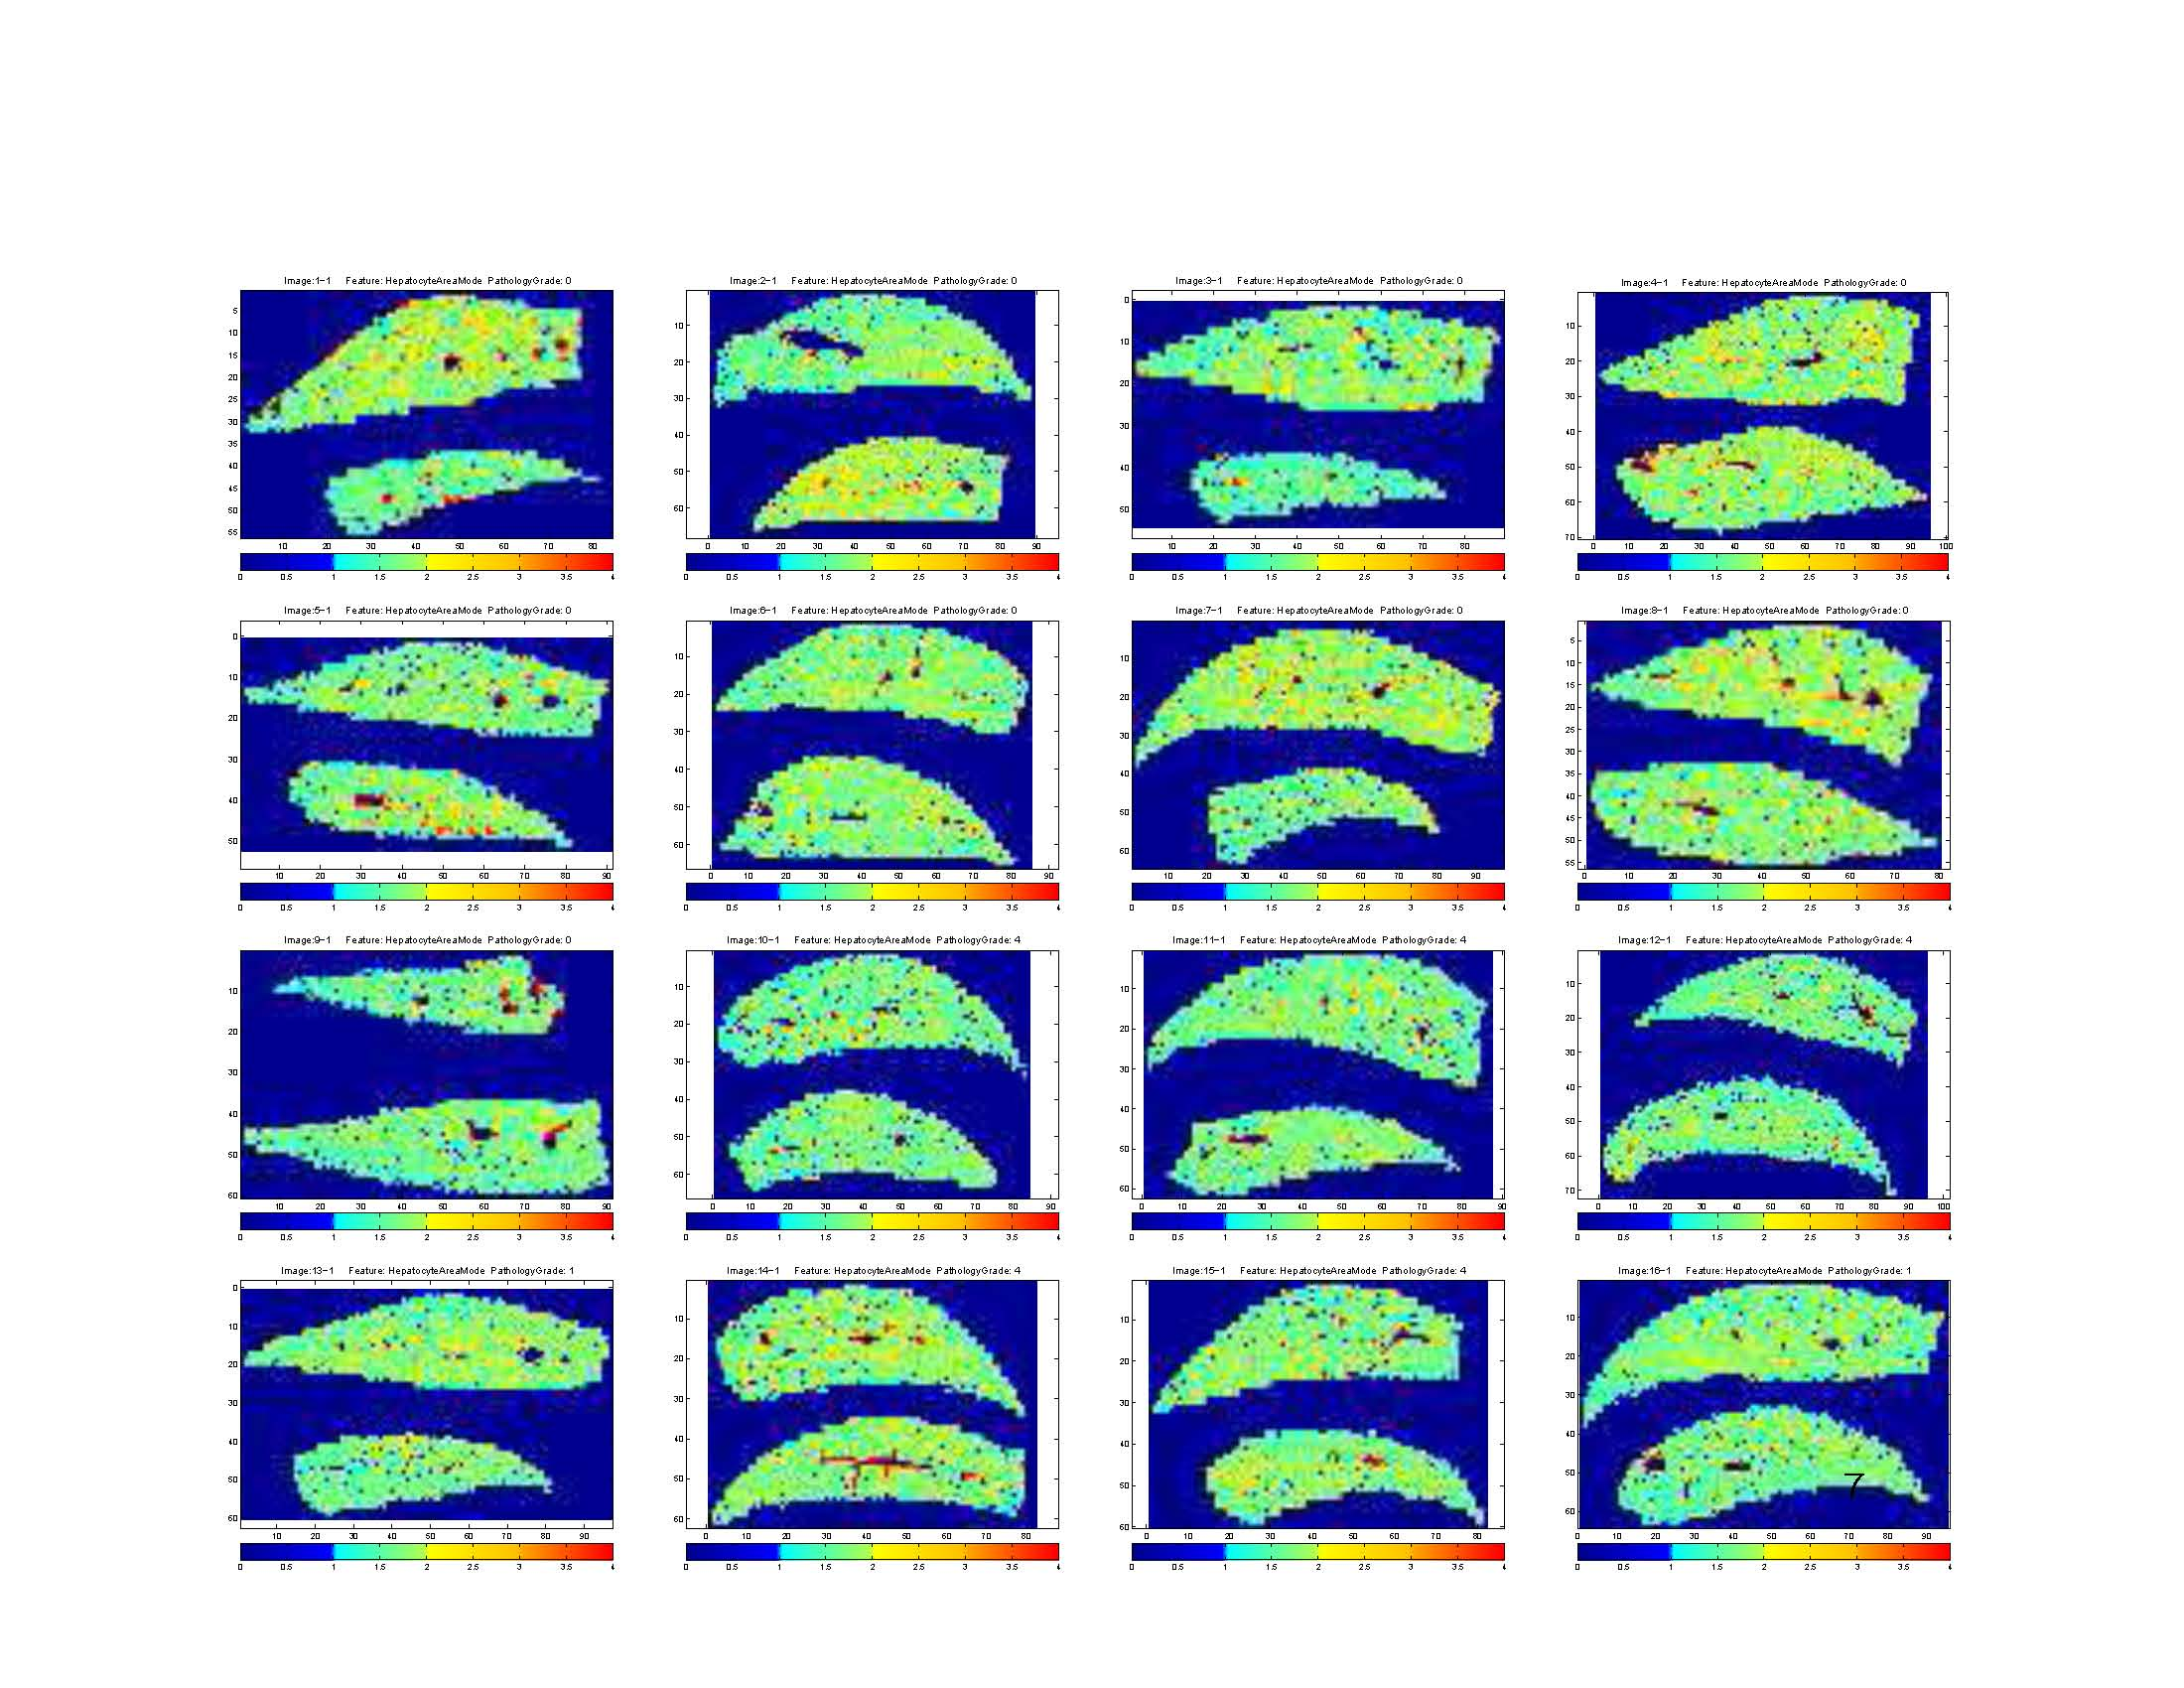
\includegraphics[width=4.0cm,height=4.0cm]{images/MachineVision/MachineVision_Pathology_ExampleSlides_Page_09.jpg} \\
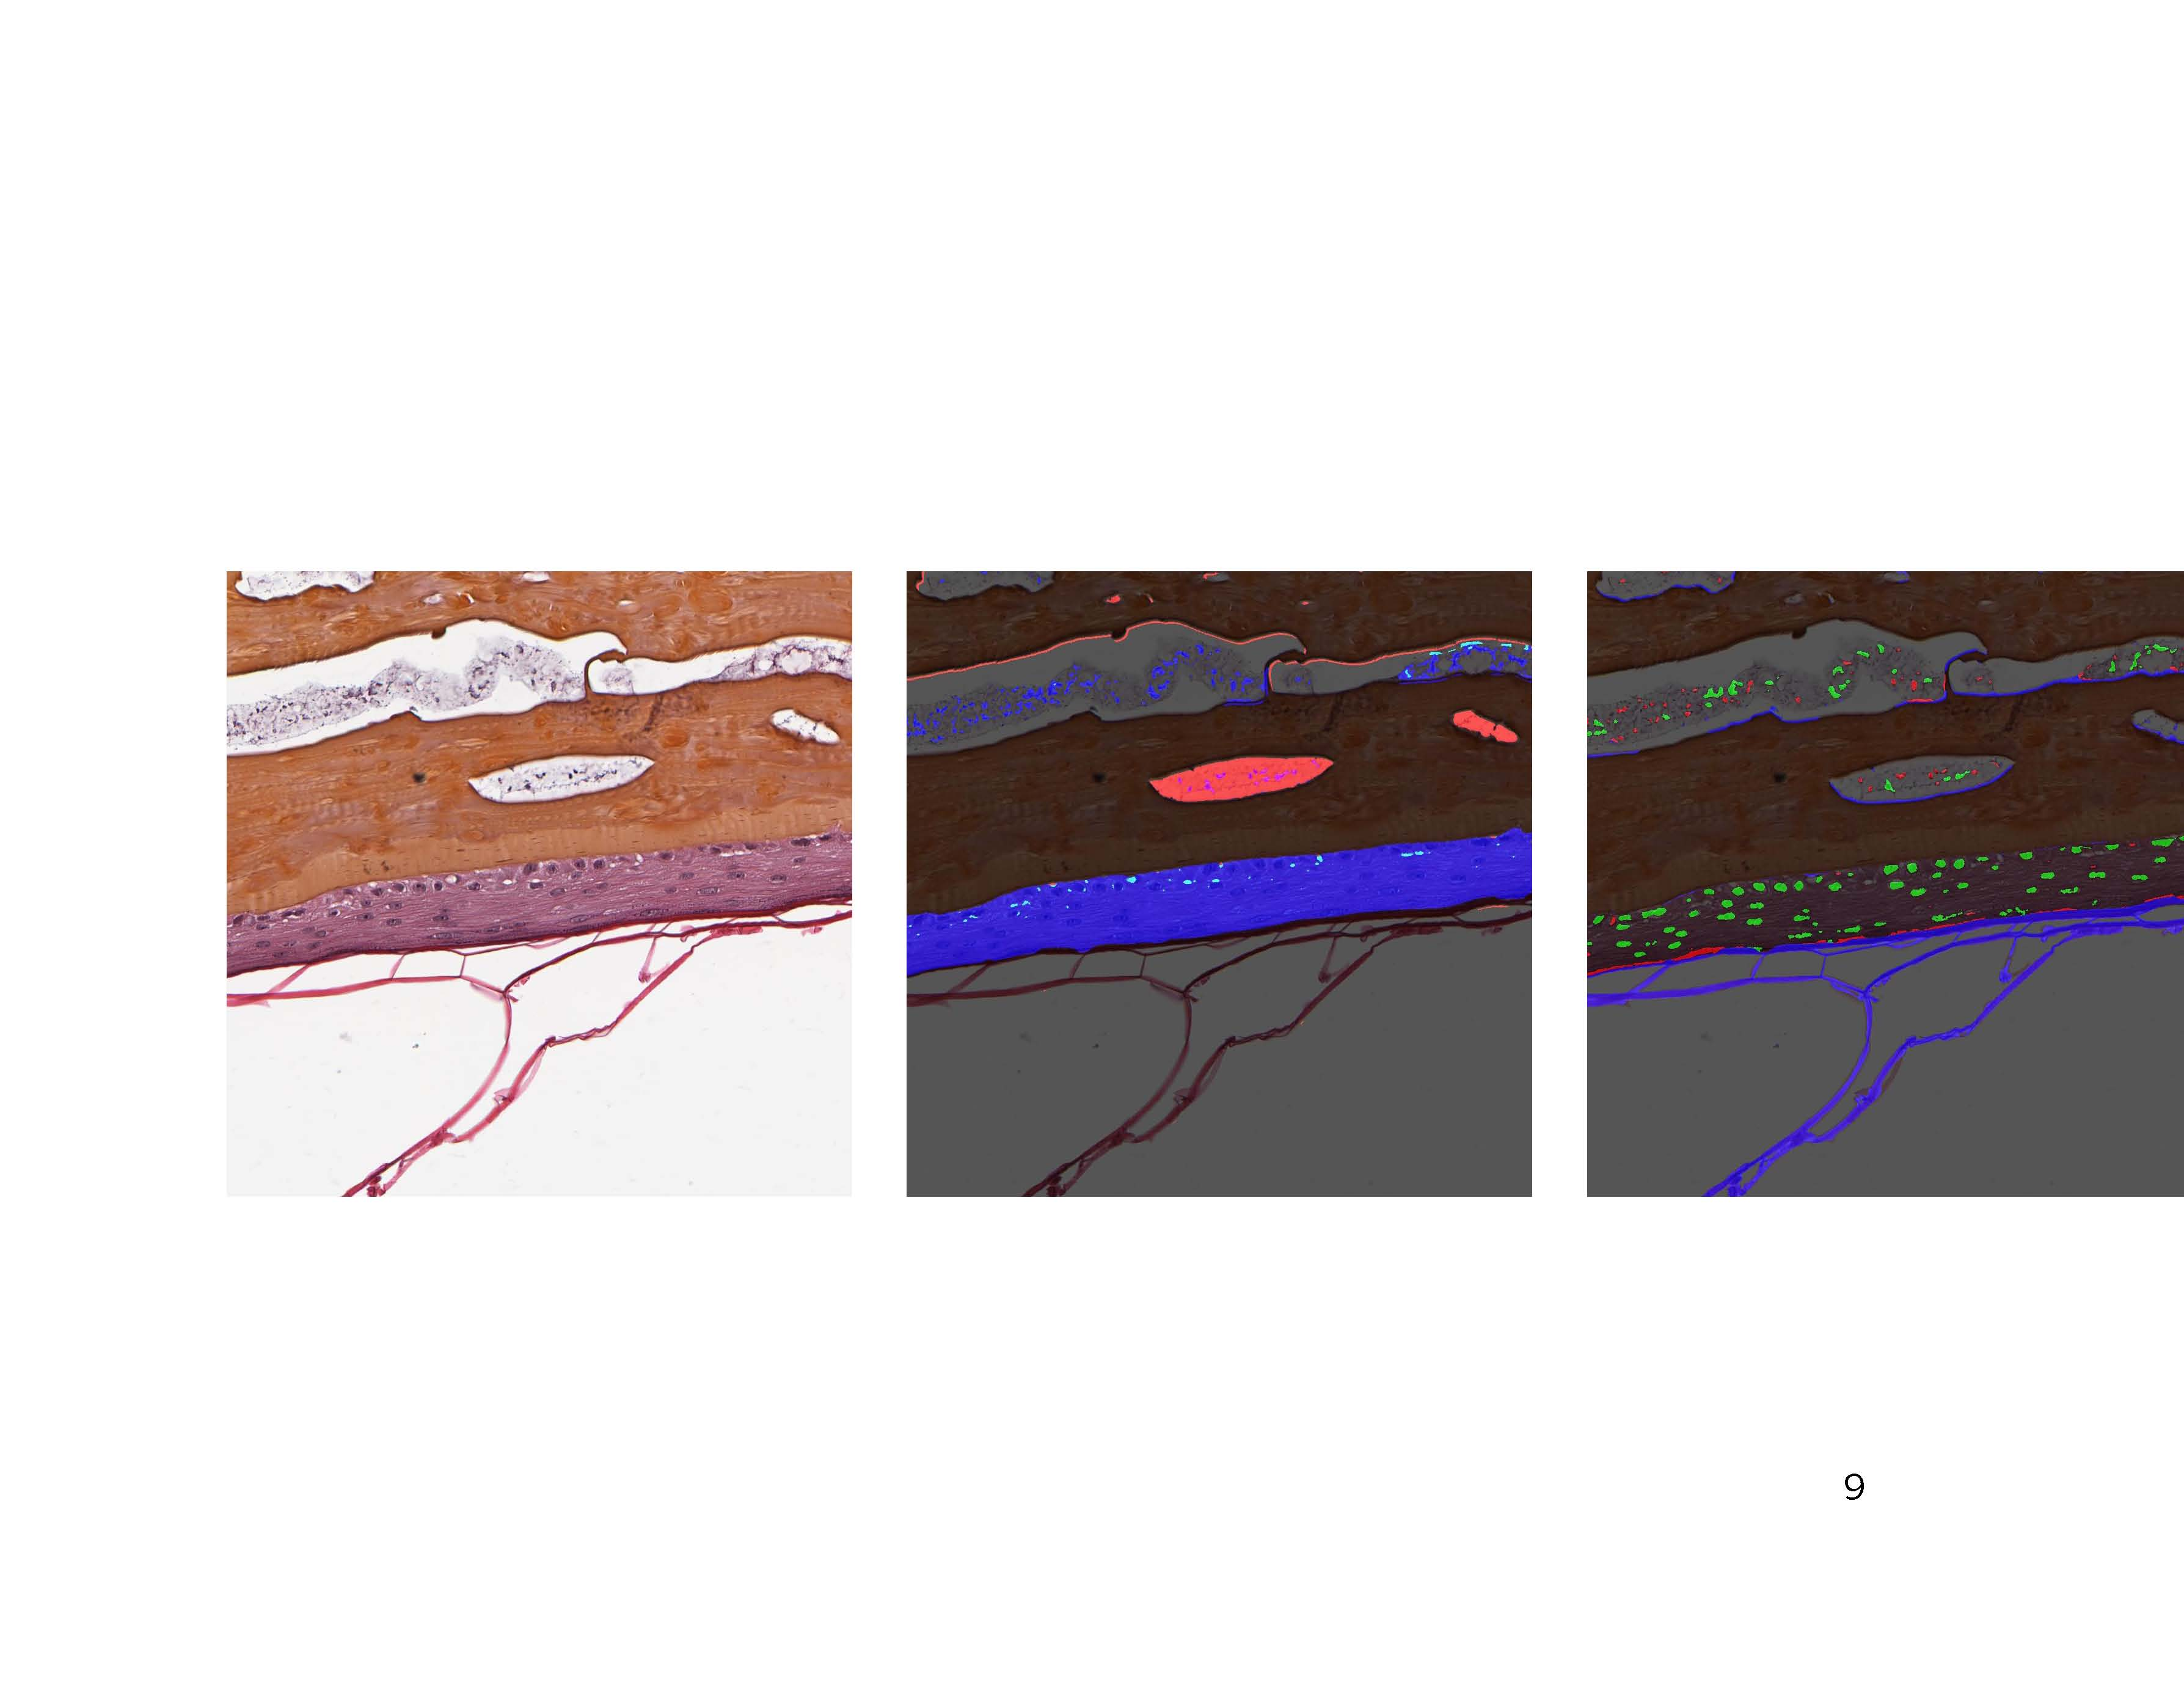
\includegraphics[width=4.0cm,height=4.0cm]{images/MachineVision/MachineVision_Pathology_ExampleSlides_Page_11.jpg} &
\includegraphics[width=4.0cm,height=4.0cm]{images/MachineVision/MachineVision_Pathology_ExampleSlides_Page_13.jpg} \\
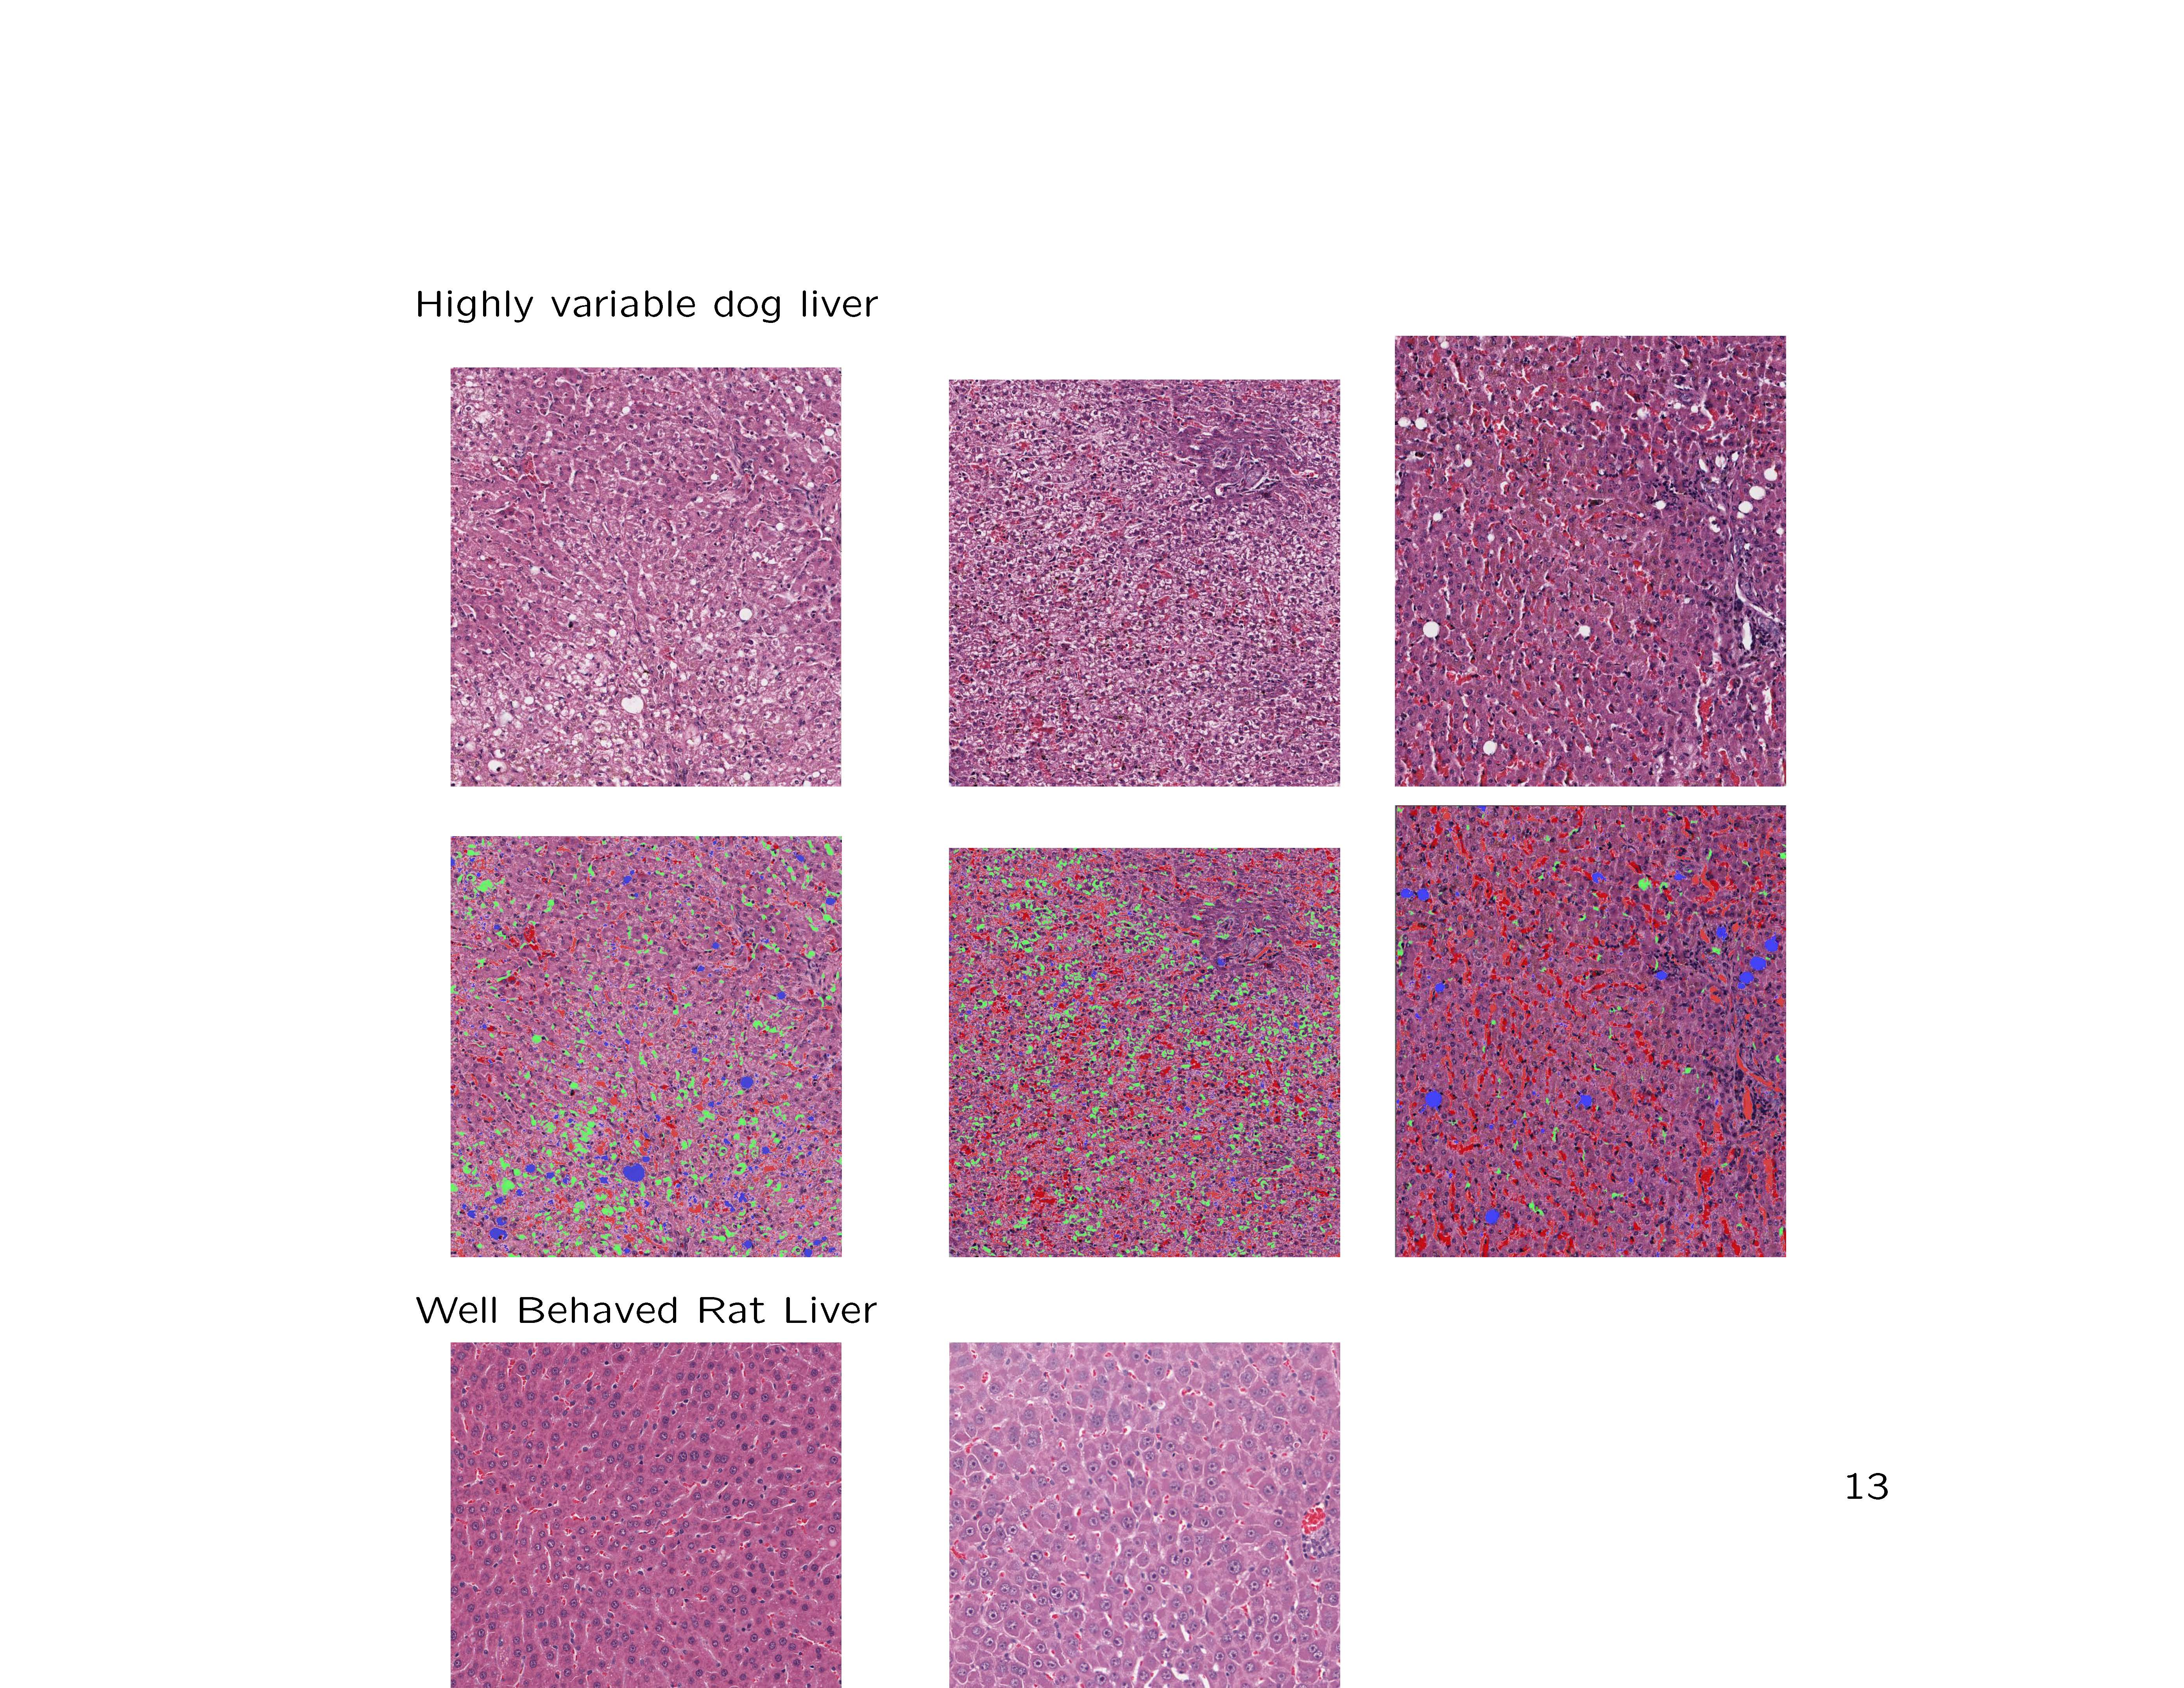
\includegraphics[width=4.0cm,height=4.0cm]{images/MachineVision/MachineVision_Pathology_ExampleSlides_Page_15.jpg} &

\includegraphics[width=4.0cm,height=4.0cm]{images/MachineVision/MachineVision_Pathology_ExampleSlides_Page_16.jpg} \end{tabular}

\section{Her2 FISH}
Her2 assessment in breast cancer provides important predictive and clinical management information. Biologic mechanisms underlying Her2 involvement in breast cancer is currently evaluated in the clinical setting via fluorescence in situ hybridization (FISH) for gene amplification and immunohistochemistry (IHC) for protein over-expression. IHC is a relatively inexpensive test and can be done in most clinical pathology labs, but grading is qualitative and subject to inter-observer variation that may have clinical implications. FISH analysis shows good concordance with high grade IHC results and can resolve inconclusive IHC results, but is expensive to implement and more laborious for the pathologist to score. This document makes the case that machine vision software can be developed to reduce the labor burden in grading Her2 FISH samples. Recent advances in slide scanning, vision software, and computer hardware bring analytical capabilities to the clinical researcher that were previously out of reach.
\subsection{The importance and challenges of accurate assessment of Her2 over-expression / amplification in metastatic breast cancer}
In 20-30\% of breast cancer cases the human epidermal growth factor receptor type 2 gene (HER-2) is over-expressed. The over-expression of Her-2 is a result of gene ampli?cation where multiple copies of the gene are present. HER2 status is predictive of disease free status post chemotherapy, and is used to identify patients most likely to benefit from Herceptin therapy. Current best practice in assessing HER2 status in metastatic breast cancer is to test for amplification using IHC and to con?rm ambiguous (2+) cases with FISH. IHC scores of 0 and 1 are assumed to be FISH negative and IHC scores of 3 are assumed to be FISH positive. There is good statistical concordance between the 0,1, and 3 IHC and FISH scores, but it is not 100\%. The subjective nature of IHC grading allows for the possibility that some IHC grade 0 and 1 cases would be HER2 positive by FISH. For background information and statistical results see  \cite{HER2FISH1} \cite{HER2FISH3} \cite{HER2FISH4} \cite{HER2FISH5} \cite{HER2FISH6} \cite{HER2FISH7} \cite{HER2FISH8}.
\subsection{ Automated \& Semi Automated Pathology}
Digital pathology is defned as the software and hardware systems designed to aid in the capture, storage, visualization, and annotation of pathology images. Automated pathology is defined as digital pathology with machine vision capabilities and is further characterized as:
\begin{itemize}
  \item semi-automated systems which assist the pathologist with functionality to improve the ability to grade via color segmentation, measurement, and counting algorithms
  \item fully automated with the ability produce whole slide grades based on statistical models built upon machine vision object classification results Challenges in developing fully automated scoring systems include
  \item The visual complexity and high degree of variation in biological images which is a challenge to developing accurate tissue segmentation software
      \item The difficulty and expense in obtaining sufficient training and test data for developing grading software.
  \item Accommodating the color and morphometric variation due to operator/equipment induced variations in staining, tissue preparation, and image capture.
  \item The subjective nature of some tests make it impossible to obtain ground truth data to benchmark performance.
\end{itemize}


It has been demonstrated that whole slide digital scanning and display does not affect the ability to make reliable clinical decisions \cite{HER2FISH2} \cite{HER2FISH3} \cite{HER2FISH4} \cite{HER2FISH5} \cite{HER2FISH6} \cite{HER2FISH7} \cite{HER2FISH8}. There is an element of luck in being able to migrate a clinical test from digital pathology to automated pathology. The stain,tissue morphology and psychophysics involved in scoring must be amenable to the capture hardware, imaging software and statistical tools at hand. The functional components of an automated pathology system:
\begin{itemize}
\item 	scan / capture, annotate, store
\item color and morphological based object segmentation
\item	pixel classification - object classification
\item	image tile classification
\end{itemize}
 whole slide classification based on object statistics An ordinal scoring model based on expert data maps the object data onto a whole slide path score. Applications involving simple visual measurements such as vacuolation or thickening of a membrane are easier for machine vision scoring models. Tasks such as low grade necrosis or in?ammation that require subtle discrimination of color or texture are harder. Tasks like detecting mitosis in H\&E tissue images or micro-calcifications in mammograms are very hard for machine vision applications since they require finding few bad object among many good objects.

PathVysion (Vysis Inc.) and Inform (Ventana Medical Systems) are two commercially available tests to evaluate HER2 status. Inform is a single probe system counterstained with DAPI or PI. The PathVysion test is a two probe HER-2/CEP17 test counterstained with DAPI. Scoring of the PathVysion test is done by locating 60 tumor cells and determining the HER-2/CEP17 signal ratio. A ratio C 2.0 is the cutoff for amplifcation. For some window around the cutoff ( .2), an additional 60 nuclei are scored. The variability in a positive expression is large. The range and distribution of 2,502 HER-2/CEP17 ratios in [3] shows that the there are a lot of spots to count for an accurate assessment of an amplified sample. Some researchers bin the upper end of the ratio and grade a ratio over 2 [bbcrevisit] as a 3.

An automated spot counting system could provide more accurate measurement of high HER-2/CEP17 ratios by estimating spots from signal intensity.  Scoring of HER2 FISH samples is an ideal candidate for semi-automated pathology. The HER-2/CEP17 ratio is a quantitative score, so some of the difficulties outlined above are alleviated. Once tumor cells are located, scoring becomes a moderate machine vision task. If an H\&E reference slide is available it can be digitally registered with the FISH image, and a pathologist selected region of interest (ROI) on an H\&E area containing tumor cells is easily mapped onto the FISH image. The expression of 3-5 signals per nucleus is a threshold of clinical importance. A computer vision system that scans whole slide FISH images and counts all admissible cells will help resolve that threshold.
Variance in sample preparation via staining and tissue thickness will often result variances in luminance that can make machine vision applications more challenging. By removing the luminance information and separating colors in a perceptual color space, a more robust segmentation can be achieved. FISH images are good candidates for segmenting in chromaticity space, because the colors are determined by the markers and optical ?lters -which tend to be stable colorimetrically.
Cell segmentation is accomplished on FISH image using common imaging tools if the cells are reasonably spaced apart. Once cells are segmented, they must be classi?ed as tumor cell or not. Classification can be accomplished two ways;
\begin{itemize}
\item	morphologically with characteristics provided by the test manufacturer
\item	via labeled cells obtained from the pathologist and a generic feature set tuned for cellular identification
\end{itemize}
Labeled data has the advantage of providing a ground truth for machine vision results.

\subsection{The results of a morphological cell segmentation and signal boosting of HER2 markers}

This algorithm was written in Matlab and evaluated on a small set of Her2 FISH images. The output would form the basis of cell classification and spot counting algorithms. A color transform can be applied in the direction of the cell stain color to obtain a quantitative measure of the cell stain that the pathologist sees. Curvature information on the boundary of the cells can be used to further discriminate cells that are not overlapping, but are touching each other. Overlapping cells could still provide valuable statistical information if modeled correctly.
Below is an example of a crowded image and a level set image of the DAPI stain that would form the basis of an overlapping ellipse model for cell segmentation. The edges of cells (generally) contain more DAPI stain than the center, this information can be used to better segment the cells.

With a mask of cancer cells a model for generating the HER-2/CEP17 ratio can be made. This again can be done with labeled pathologist data, or by modeling based on specifications from the FISH application. As the HER-2/CEP17 ratio rises the spots start to coalesce. Compounding this di?culty is that some FISH signals can be ghosts of real ones and must be eliminated from the count. Ghosts can be tractable for moderate amplification in that they will be an affine transform away from the real signal. Frequency based filtering methods can be used to detect ghosts. A robust statistical approach can be used to estimate the HER-2/CEP17 ratio from the spatial signal strength of the amplification.

\begin{tabular}{ |c|c|c| }
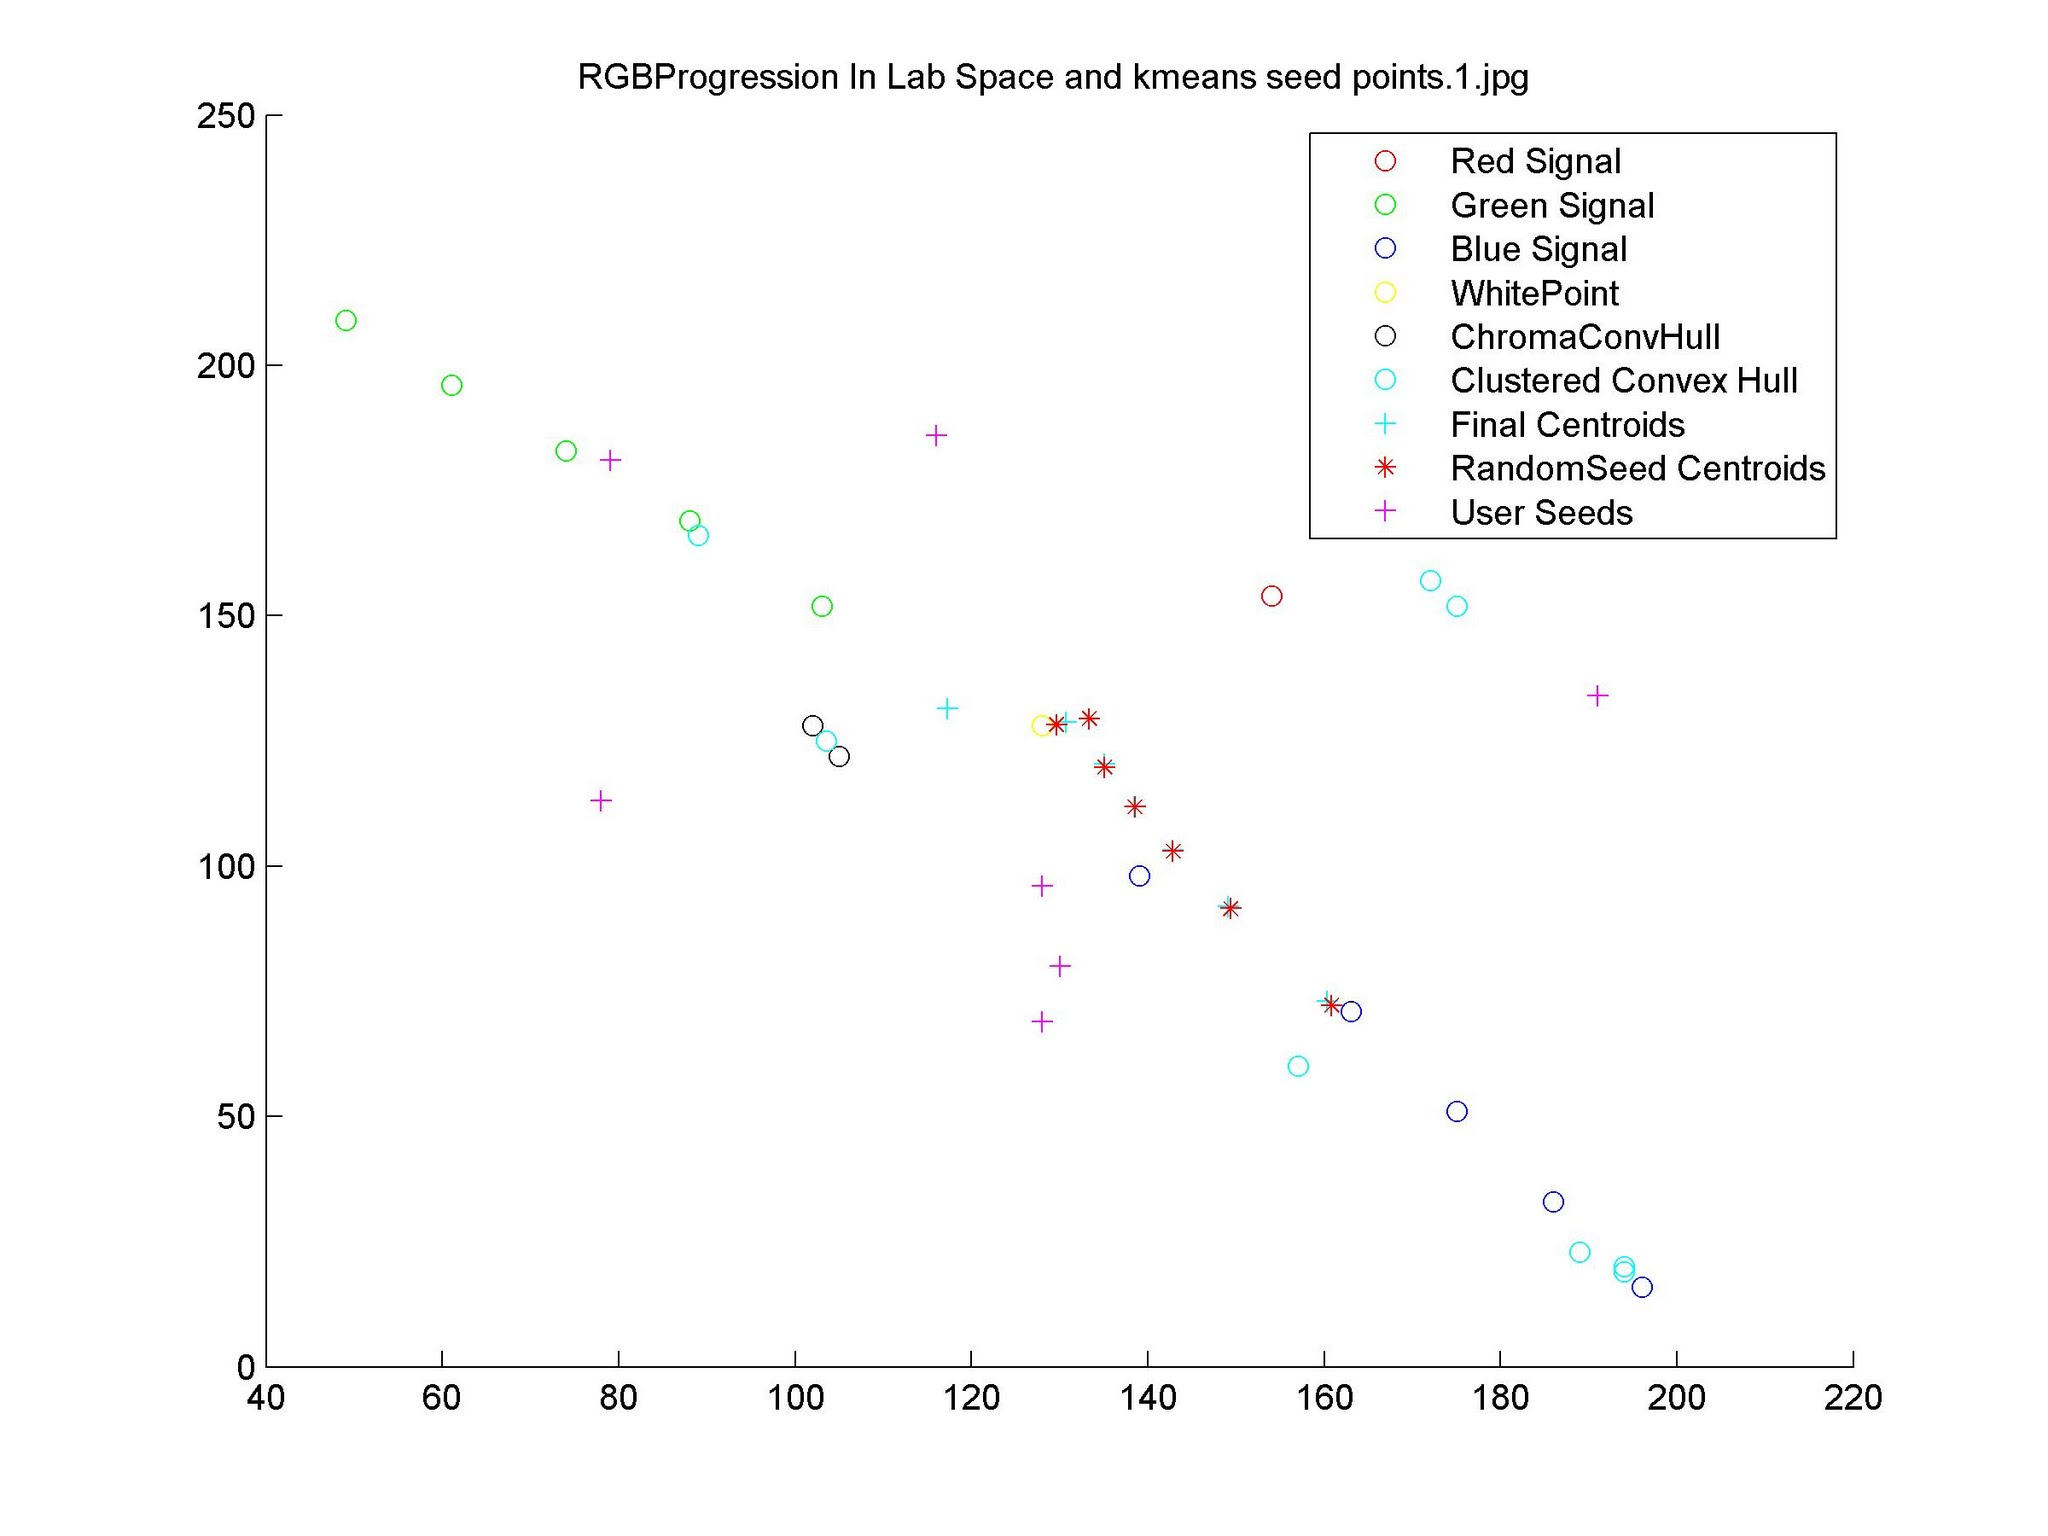
\includegraphics[width=5.0cm,height=5.0cm]{images/Her2Fish/1_abConvexHull.jpg}  &
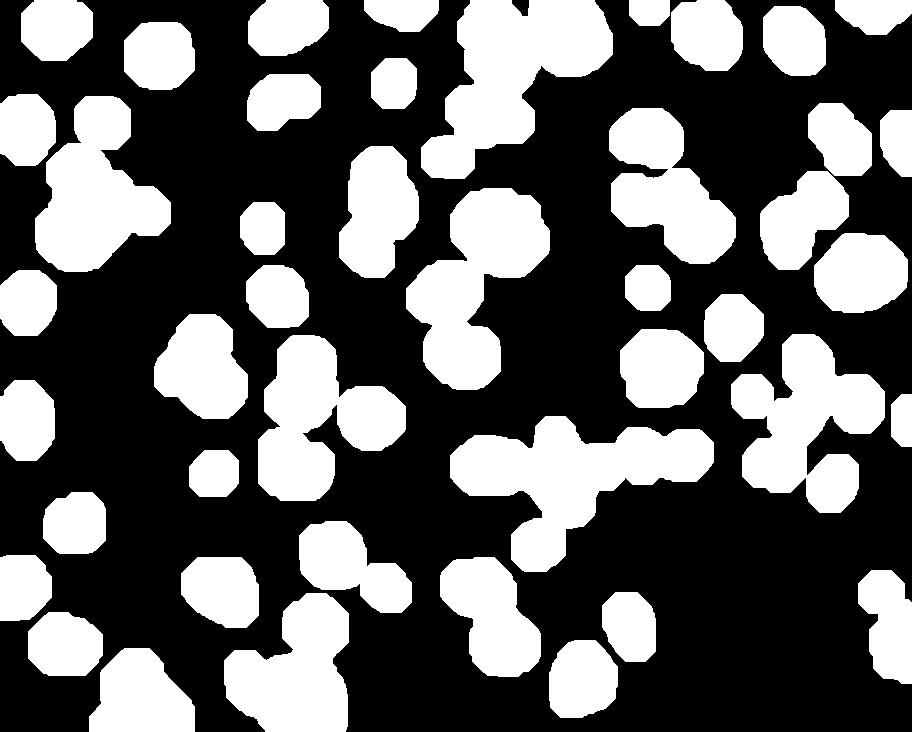
\includegraphics[width=5.0cm,height=5.0cm]{images/Her2Fish/1_Processedlabelimage.jpg}   &
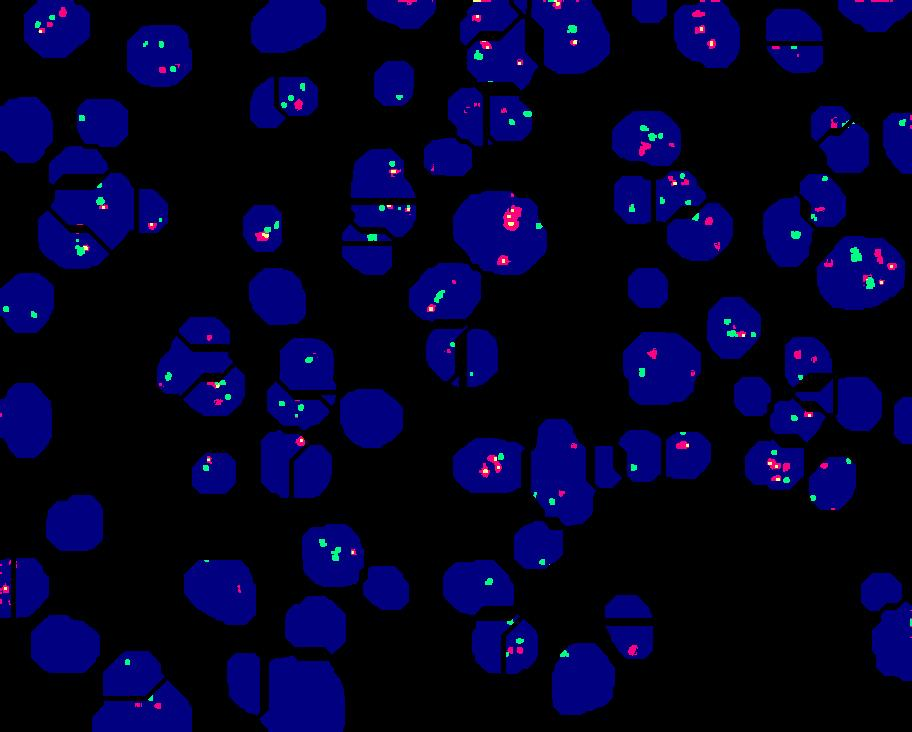
\includegraphics[width=5.0cm,height=5.0cm]{images/Her2Fish/1_RGBMASK.jpg}  \\
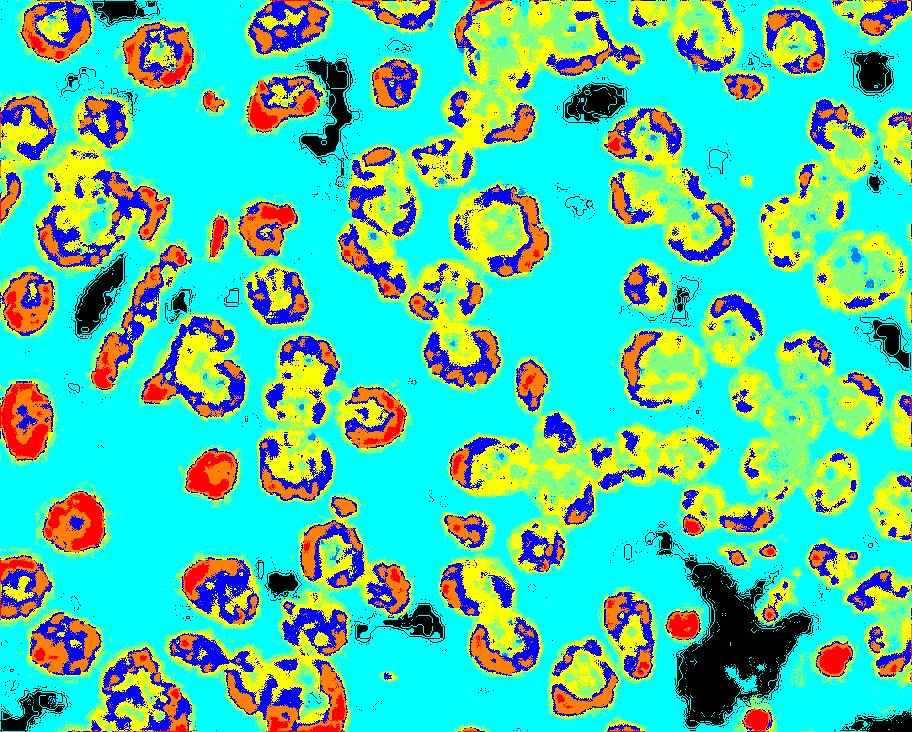
\includegraphics[width=5.0cm,height=5.0cm]{images/Her2Fish/1_RGB_LabelImg.jpg}  &
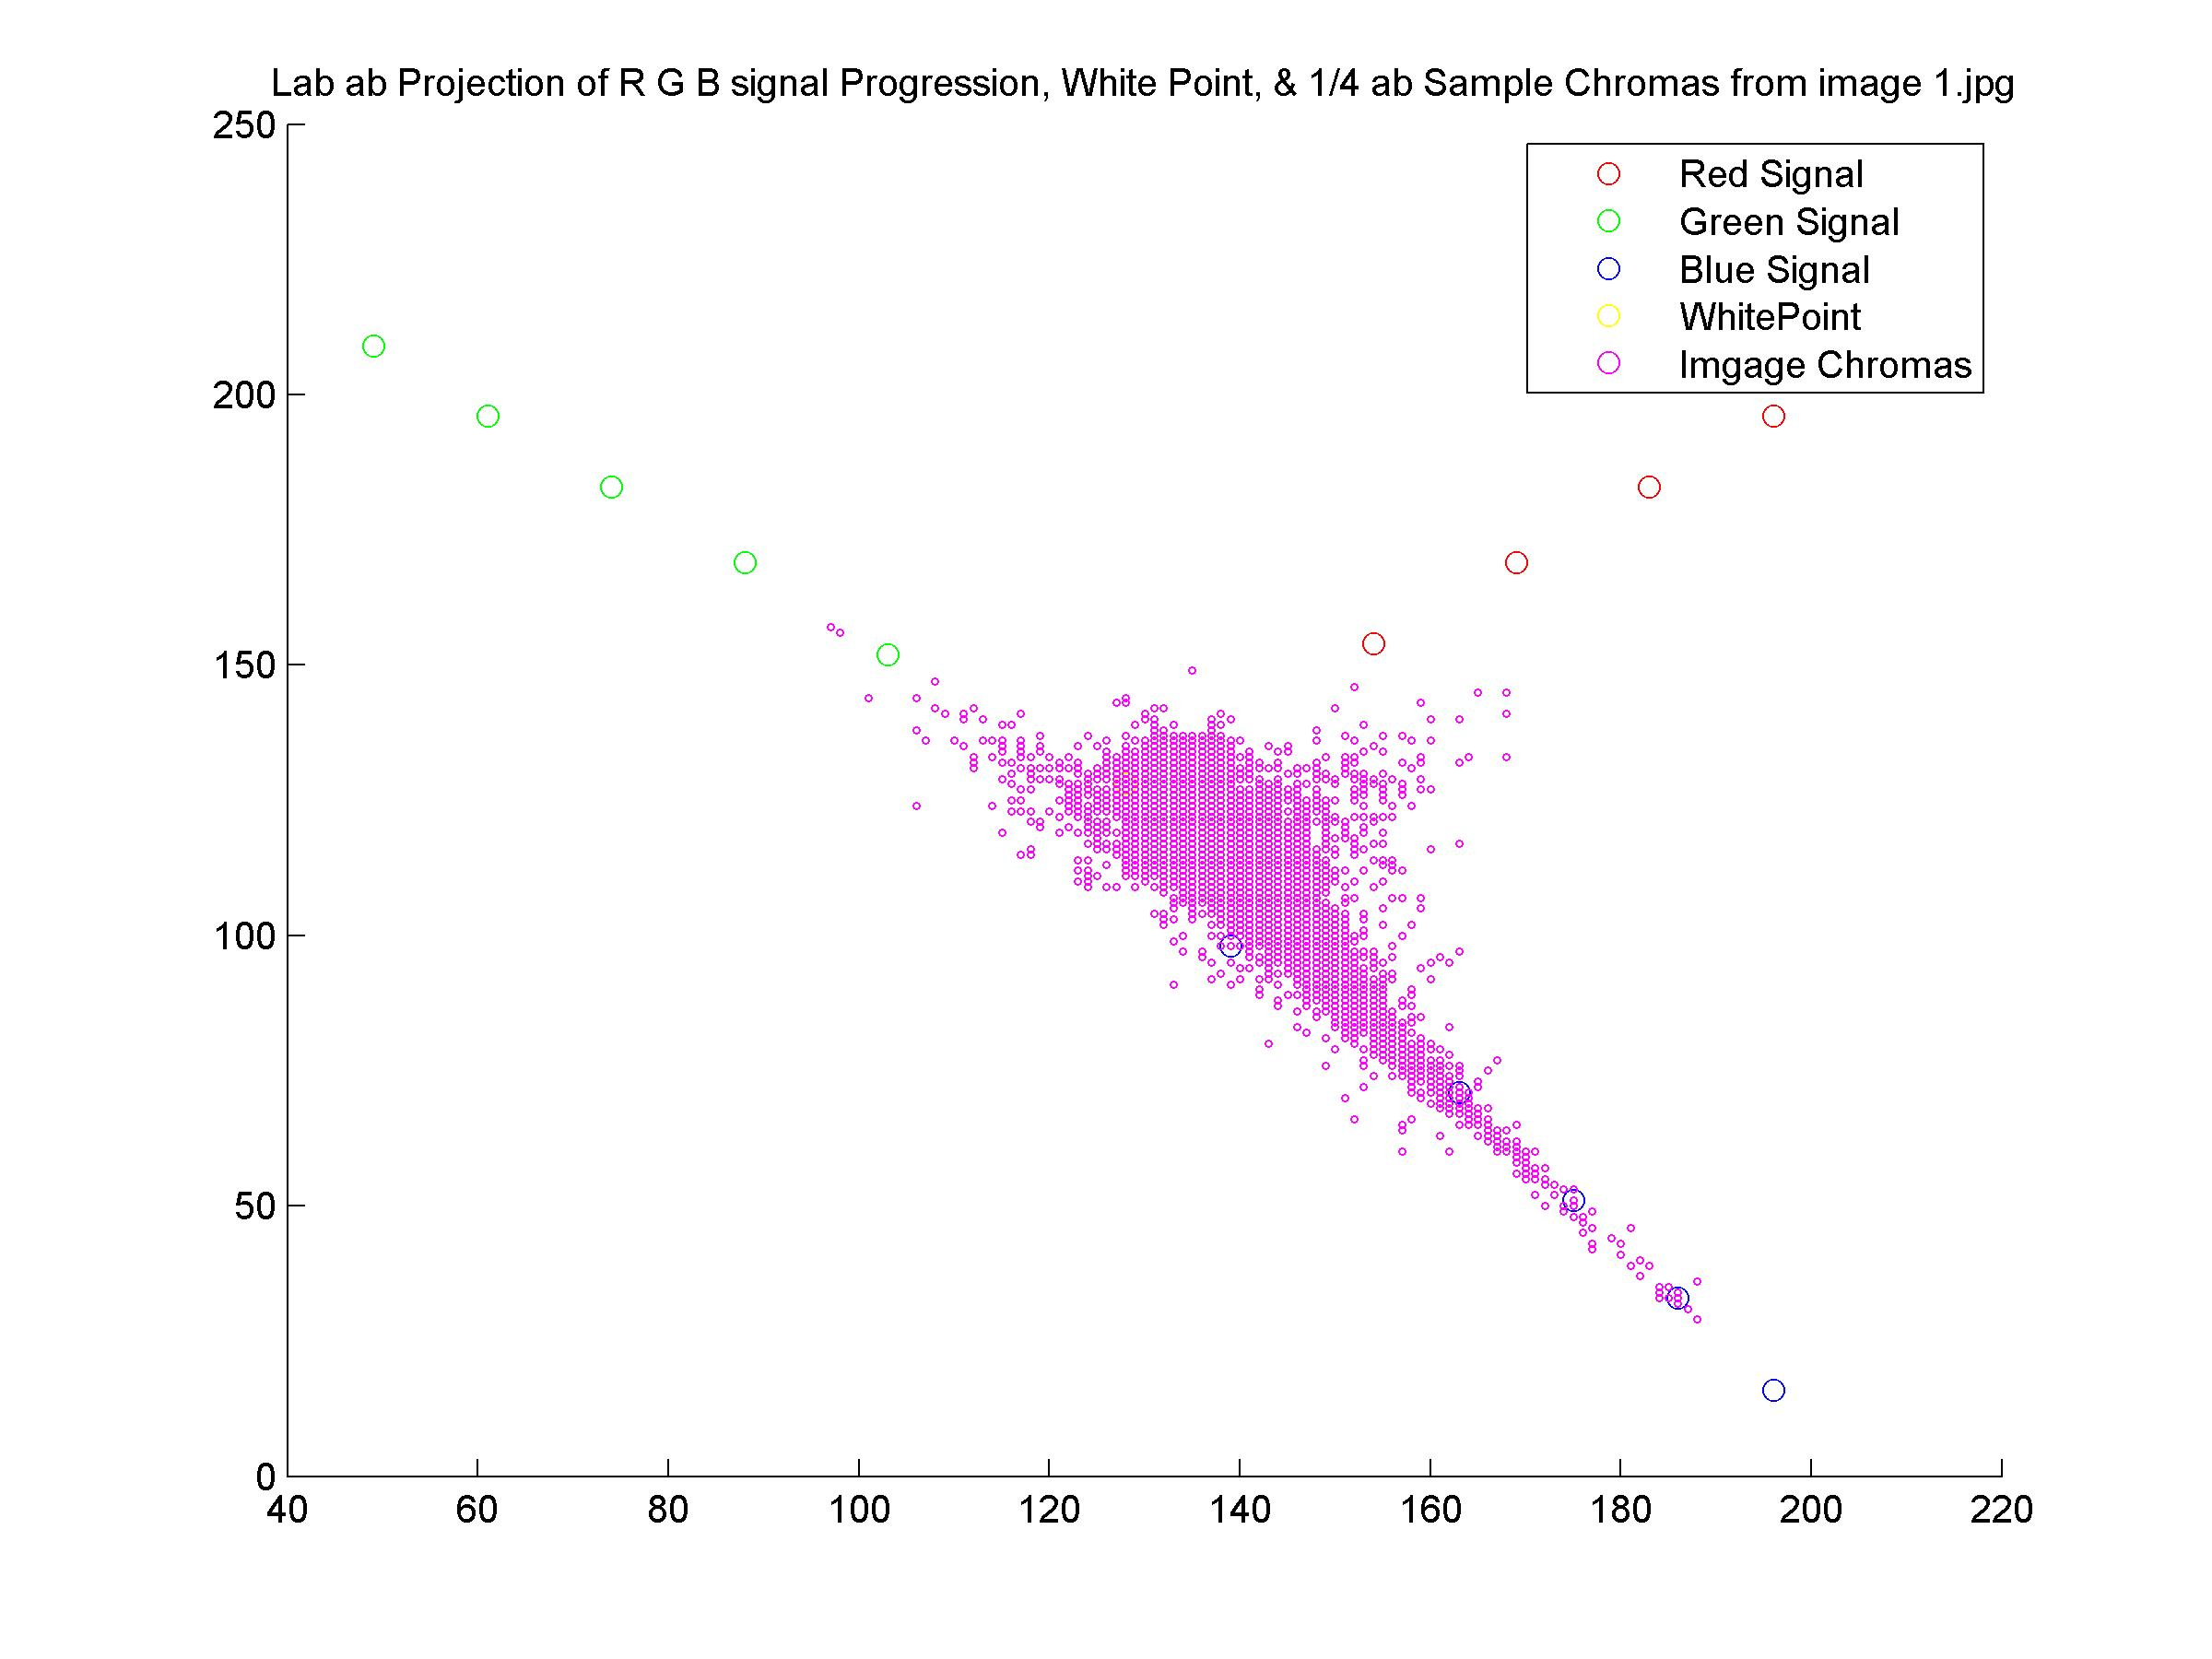
\includegraphics[width=5.0cm,height=5.0cm]{images/Her2Fish/1_SampleChromas.jpg}  &
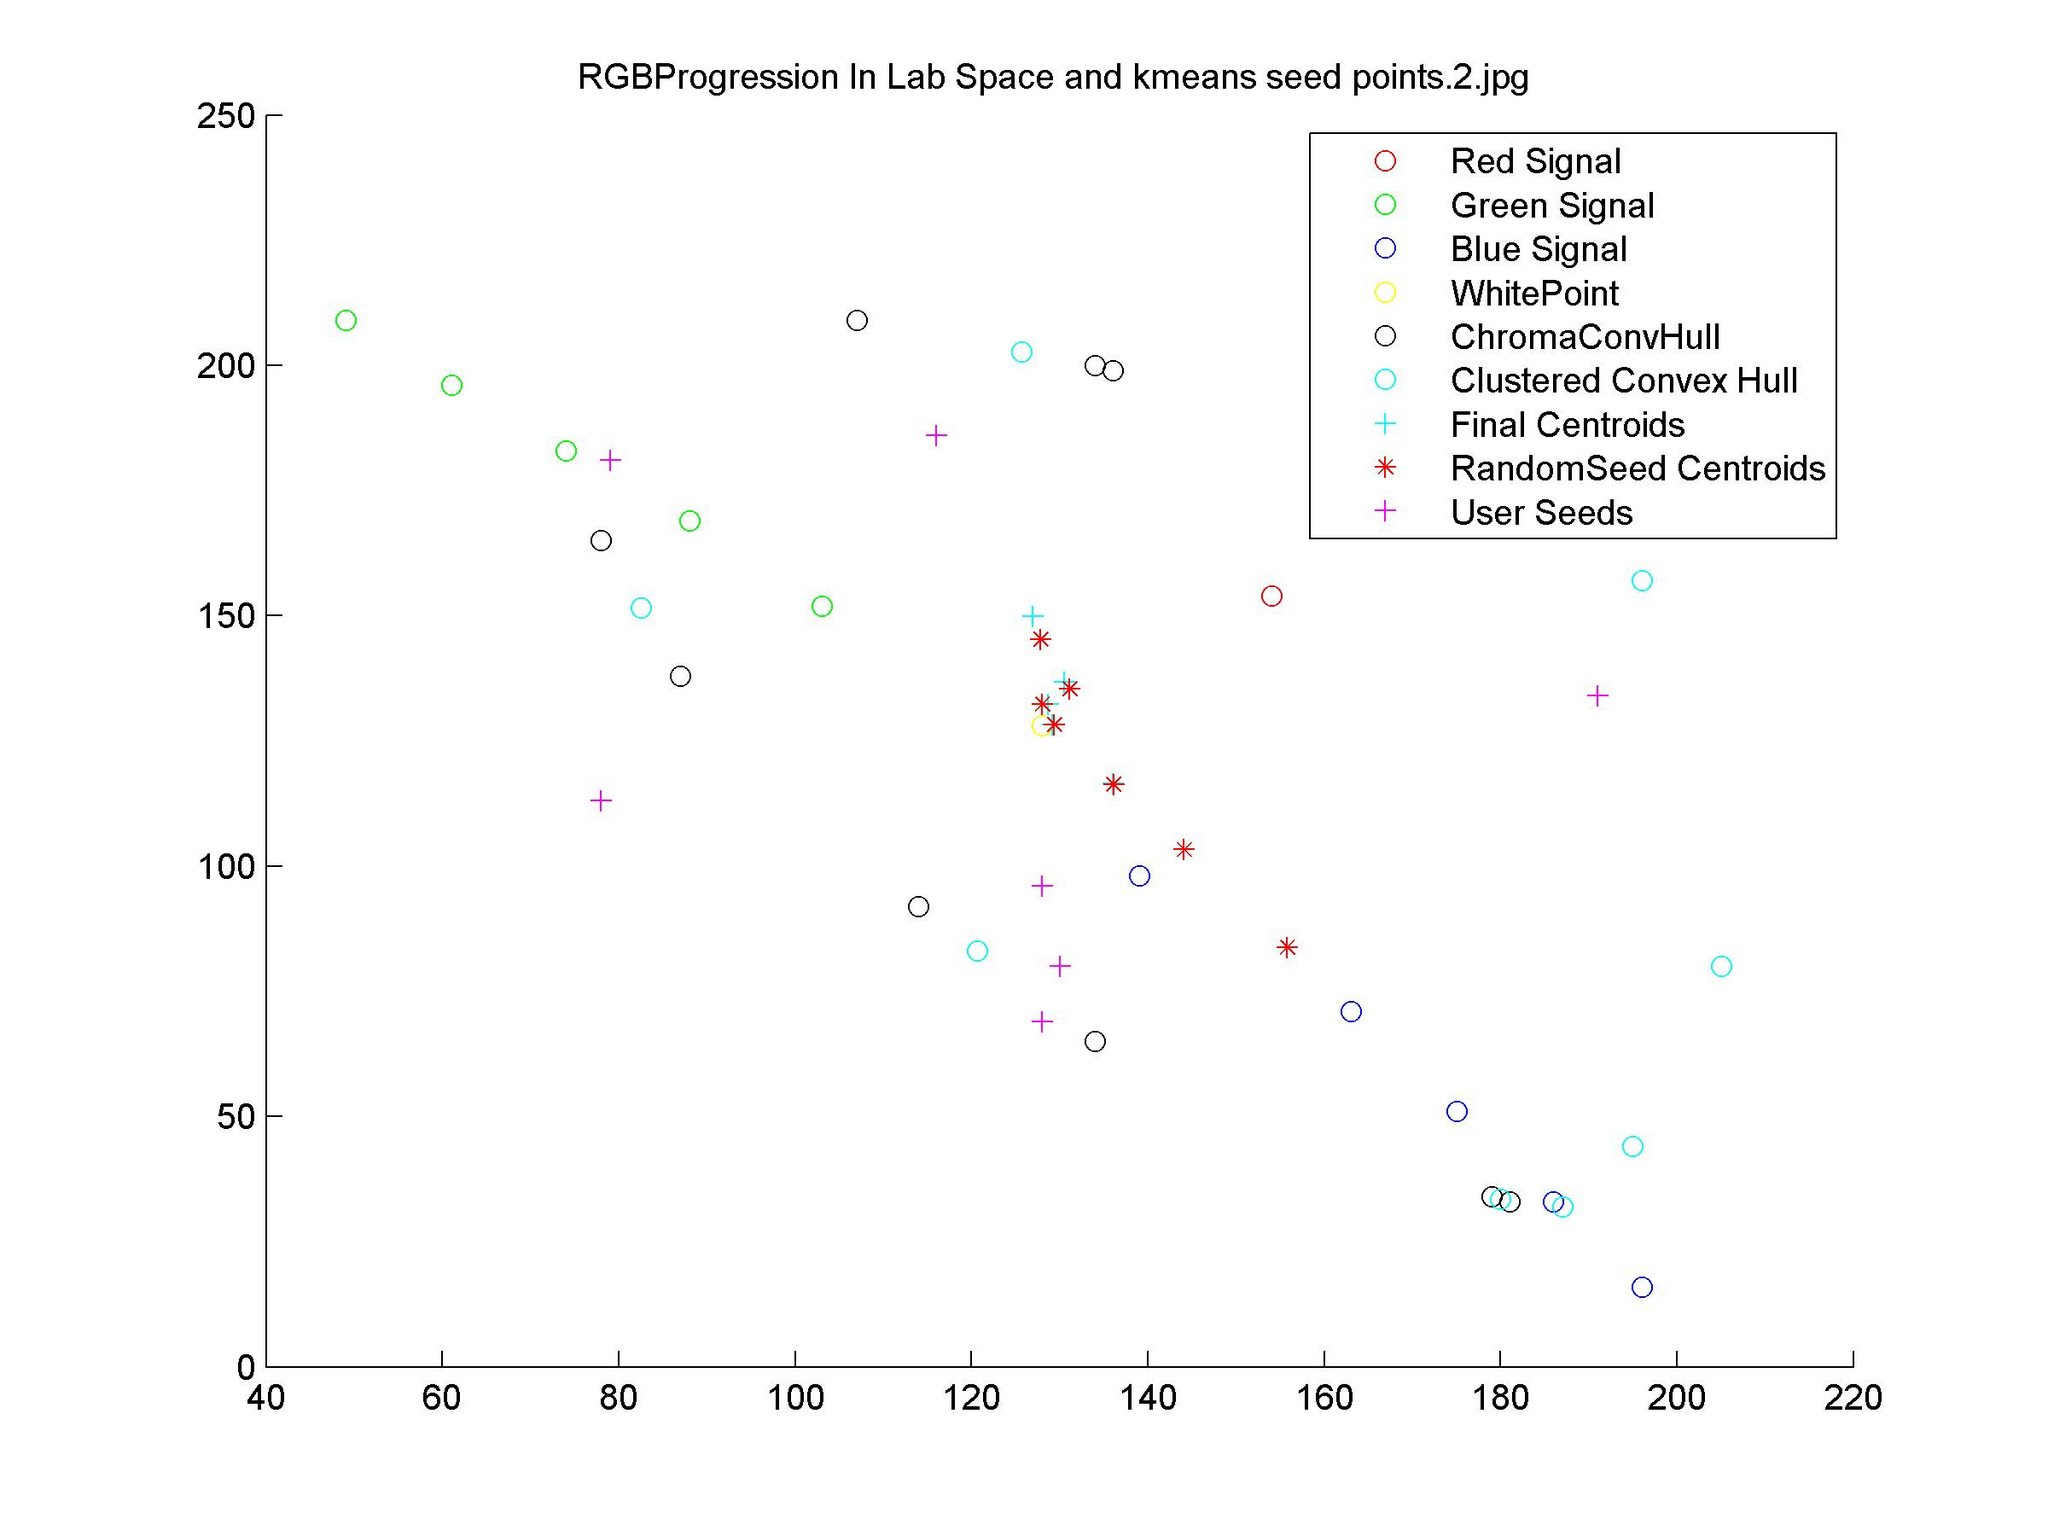
\includegraphics[width=5.0cm,height=5.0cm]{images/Her2Fish/2_abConvexHull.jpg}   \\
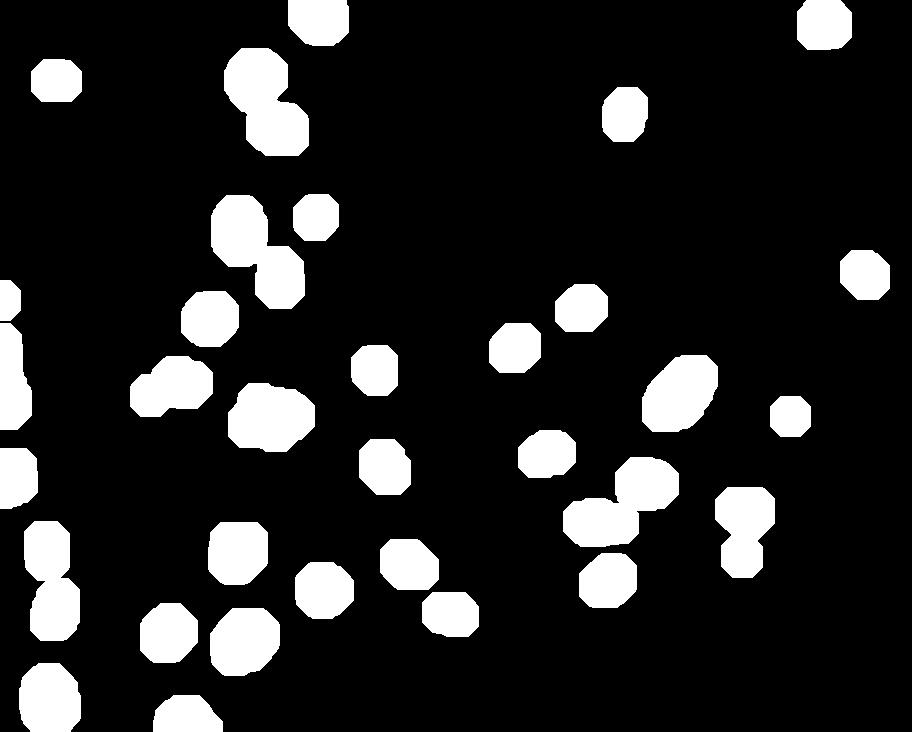
\includegraphics[width=5.0cm,height=5.0cm]{images/Her2Fish/2_Processedlabelimage.jpg}  &
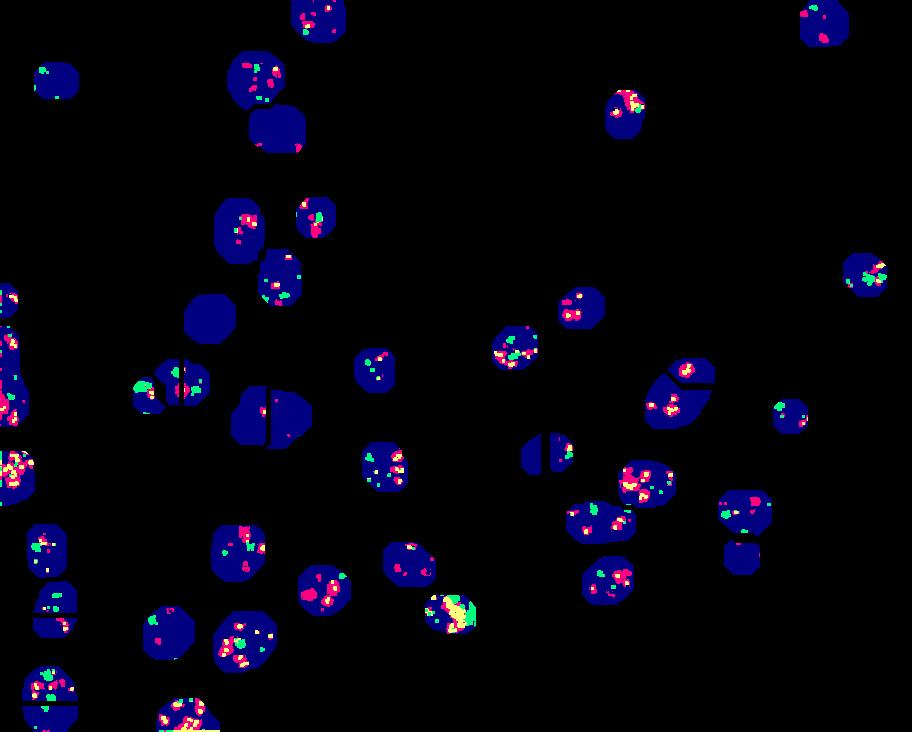
\includegraphics[width=5.0cm,height=5.0cm]{images/Her2Fish/2_RGBMASK.jpg}           &
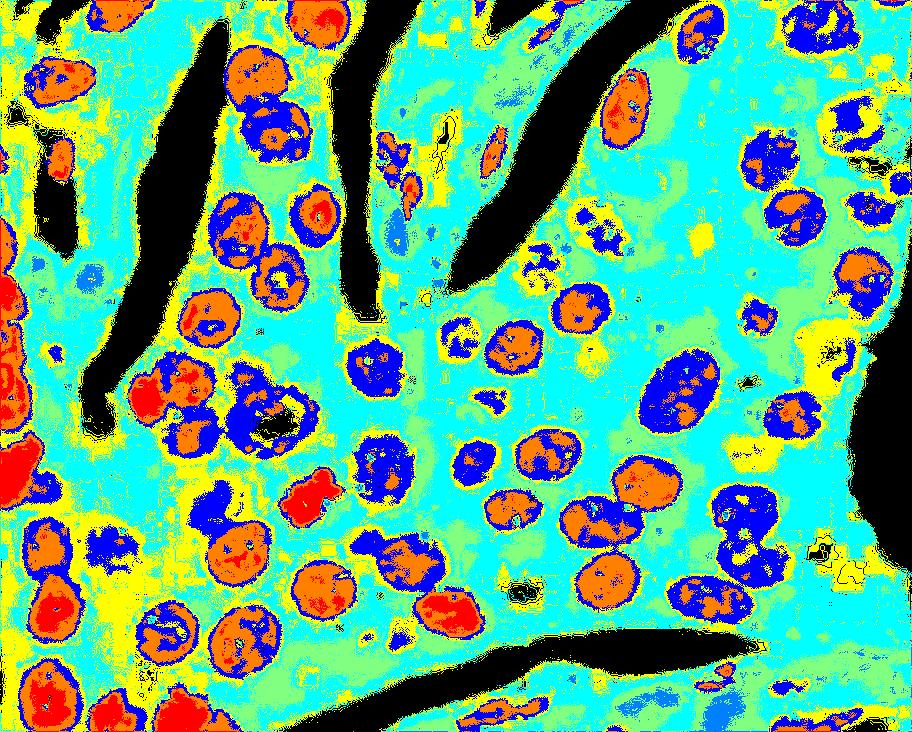
\includegraphics[width=5.0cm,height=5.0cm]{images/Her2Fish/2_RGB_LabelImg.jpg}   \\
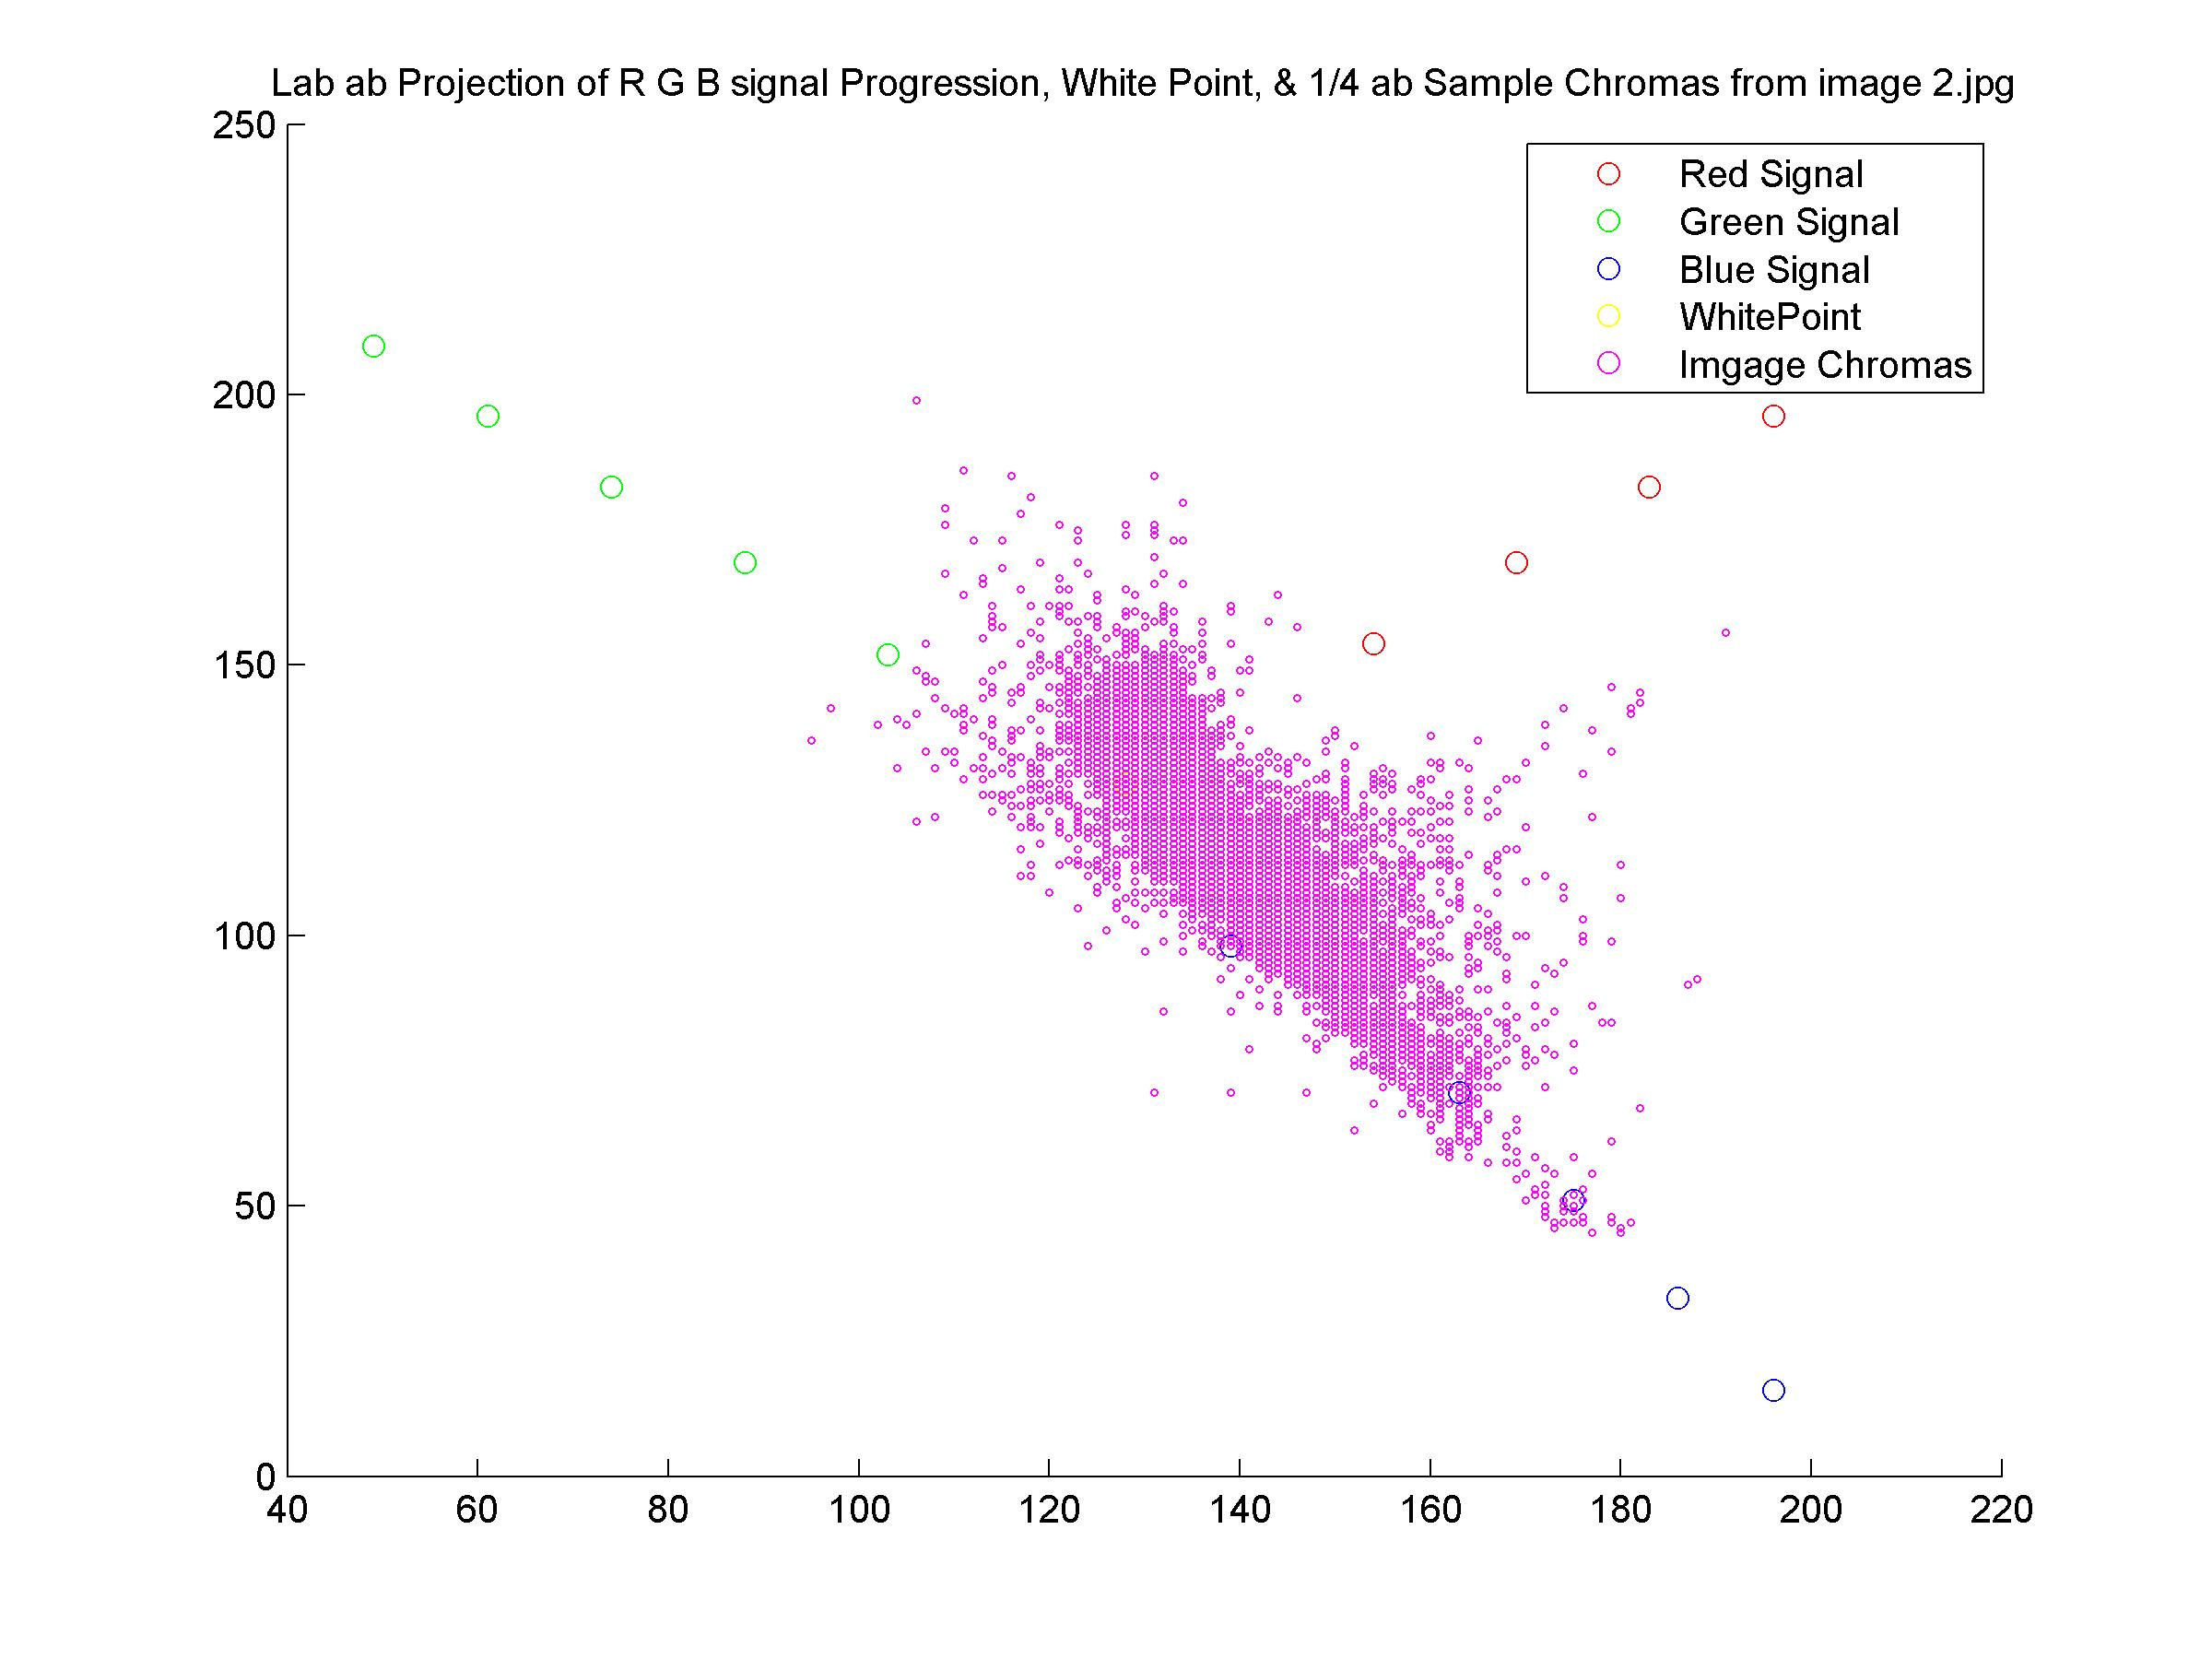
\includegraphics[width=5.0cm,height=5.0cm]{images/Her2Fish/2_SampleChromas.jpg}   &
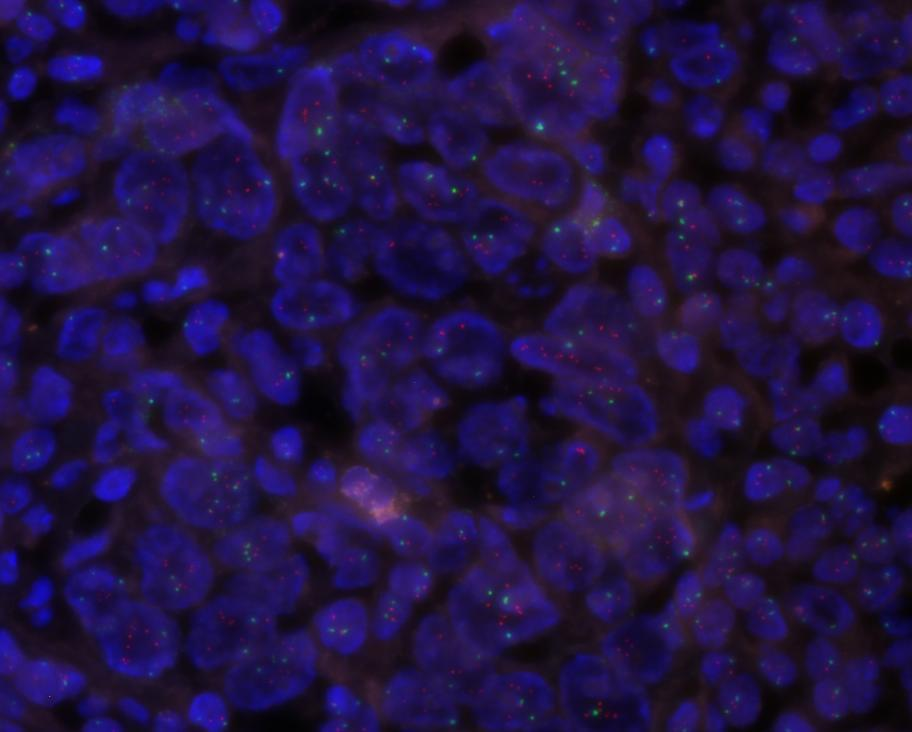
\includegraphics[width=5.0cm,height=5.0cm]{images/Her2Fish/3.jpg}
\end{tabular}


\begin{tabular}{ |c|c|c| }
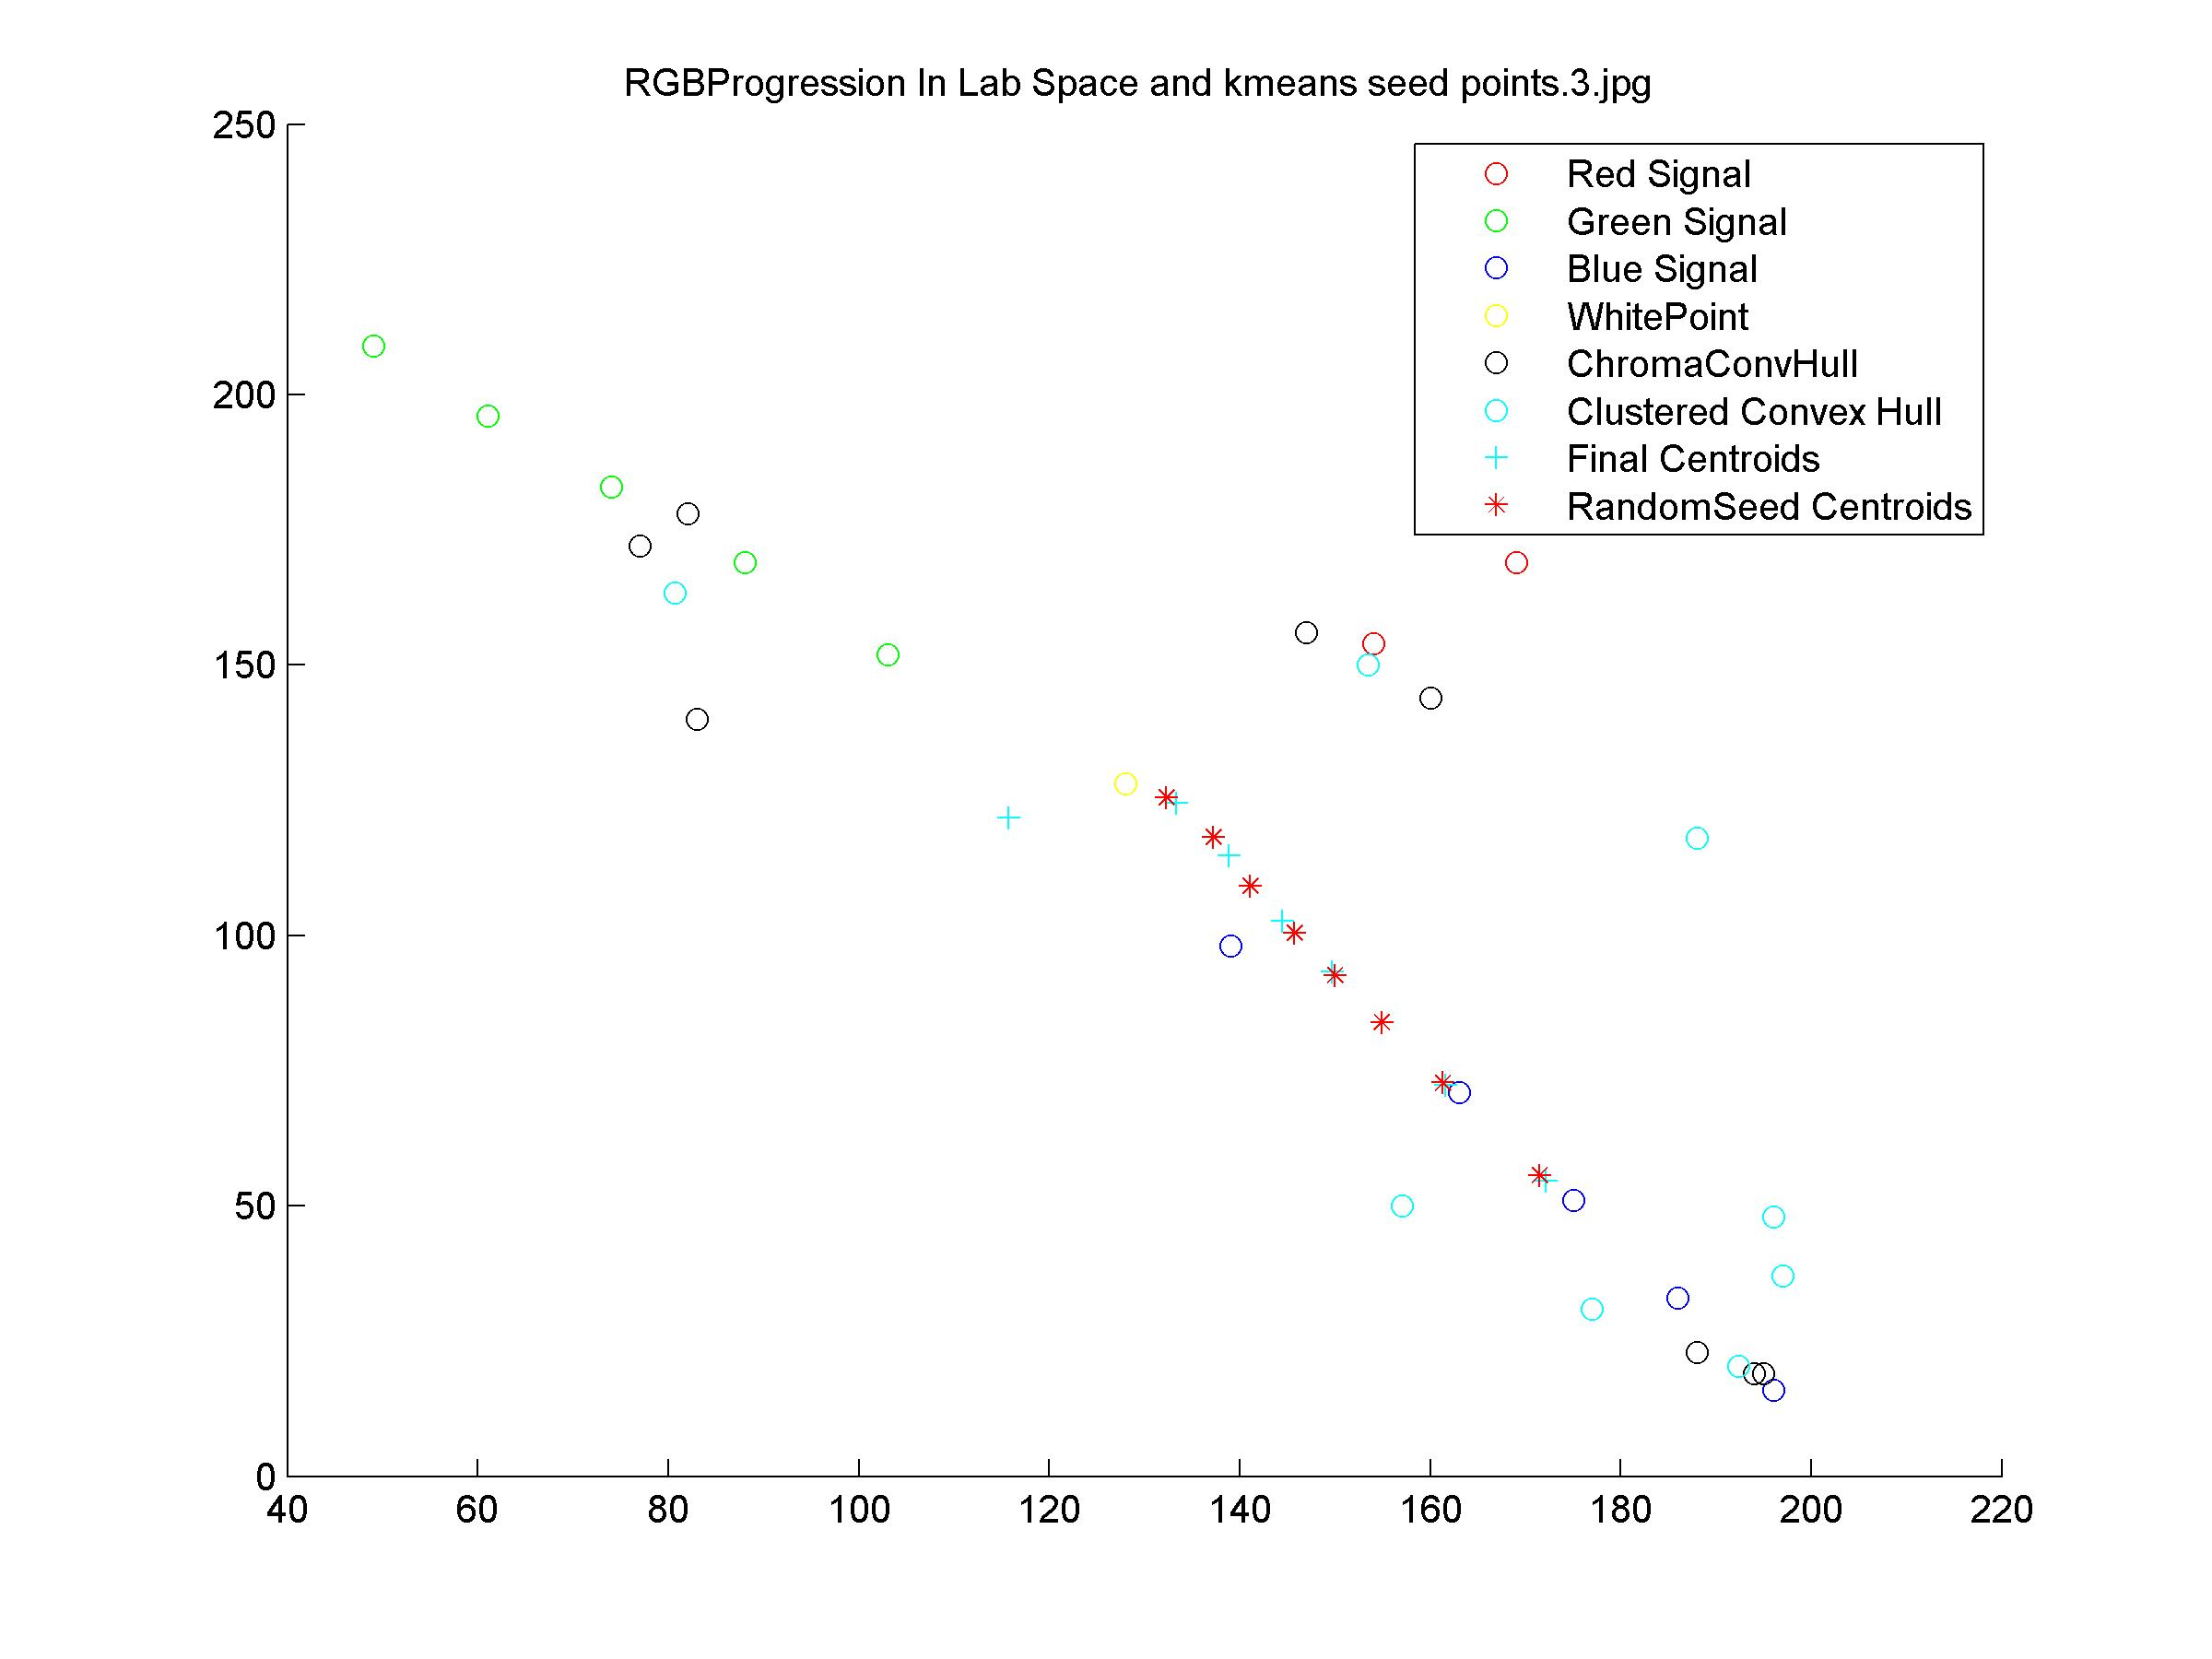
\includegraphics[width=5.0cm,height=5.0cm]{images/Her2Fish/3_abConvexHull.jpg} \\
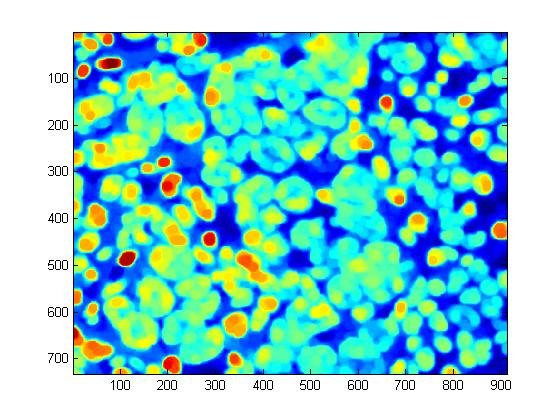
\includegraphics[width=5.0cm,height=5.0cm]{images/Her2Fish/3_BlueMaskOpen.jpg}   &
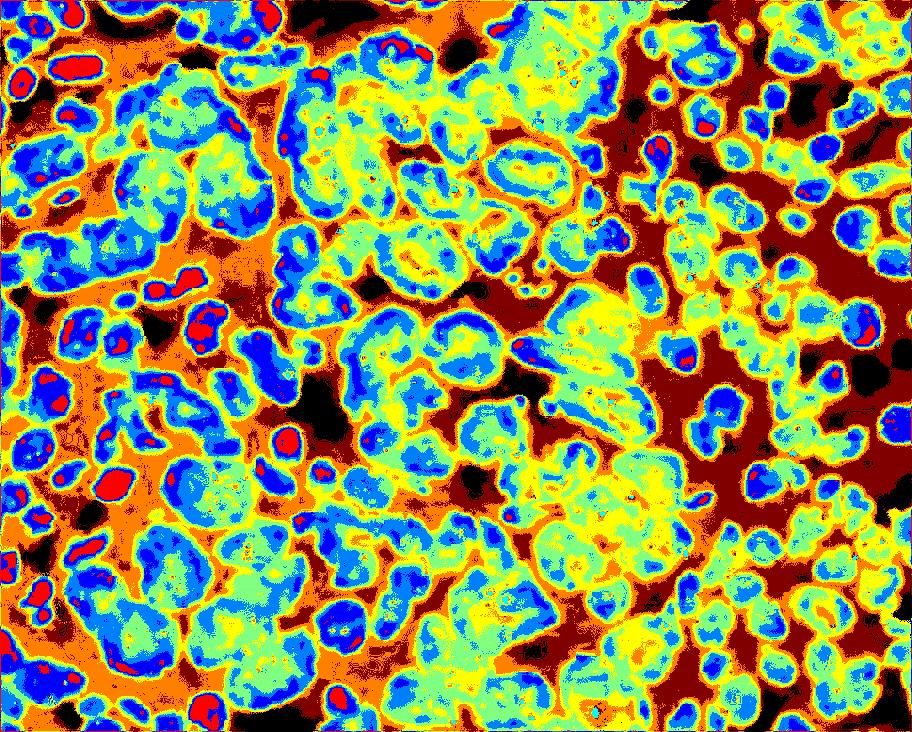
\includegraphics[width=5.0cm,height=5.0cm]{images/Her2Fish/3_RGB_LabelImg.jpg}    &
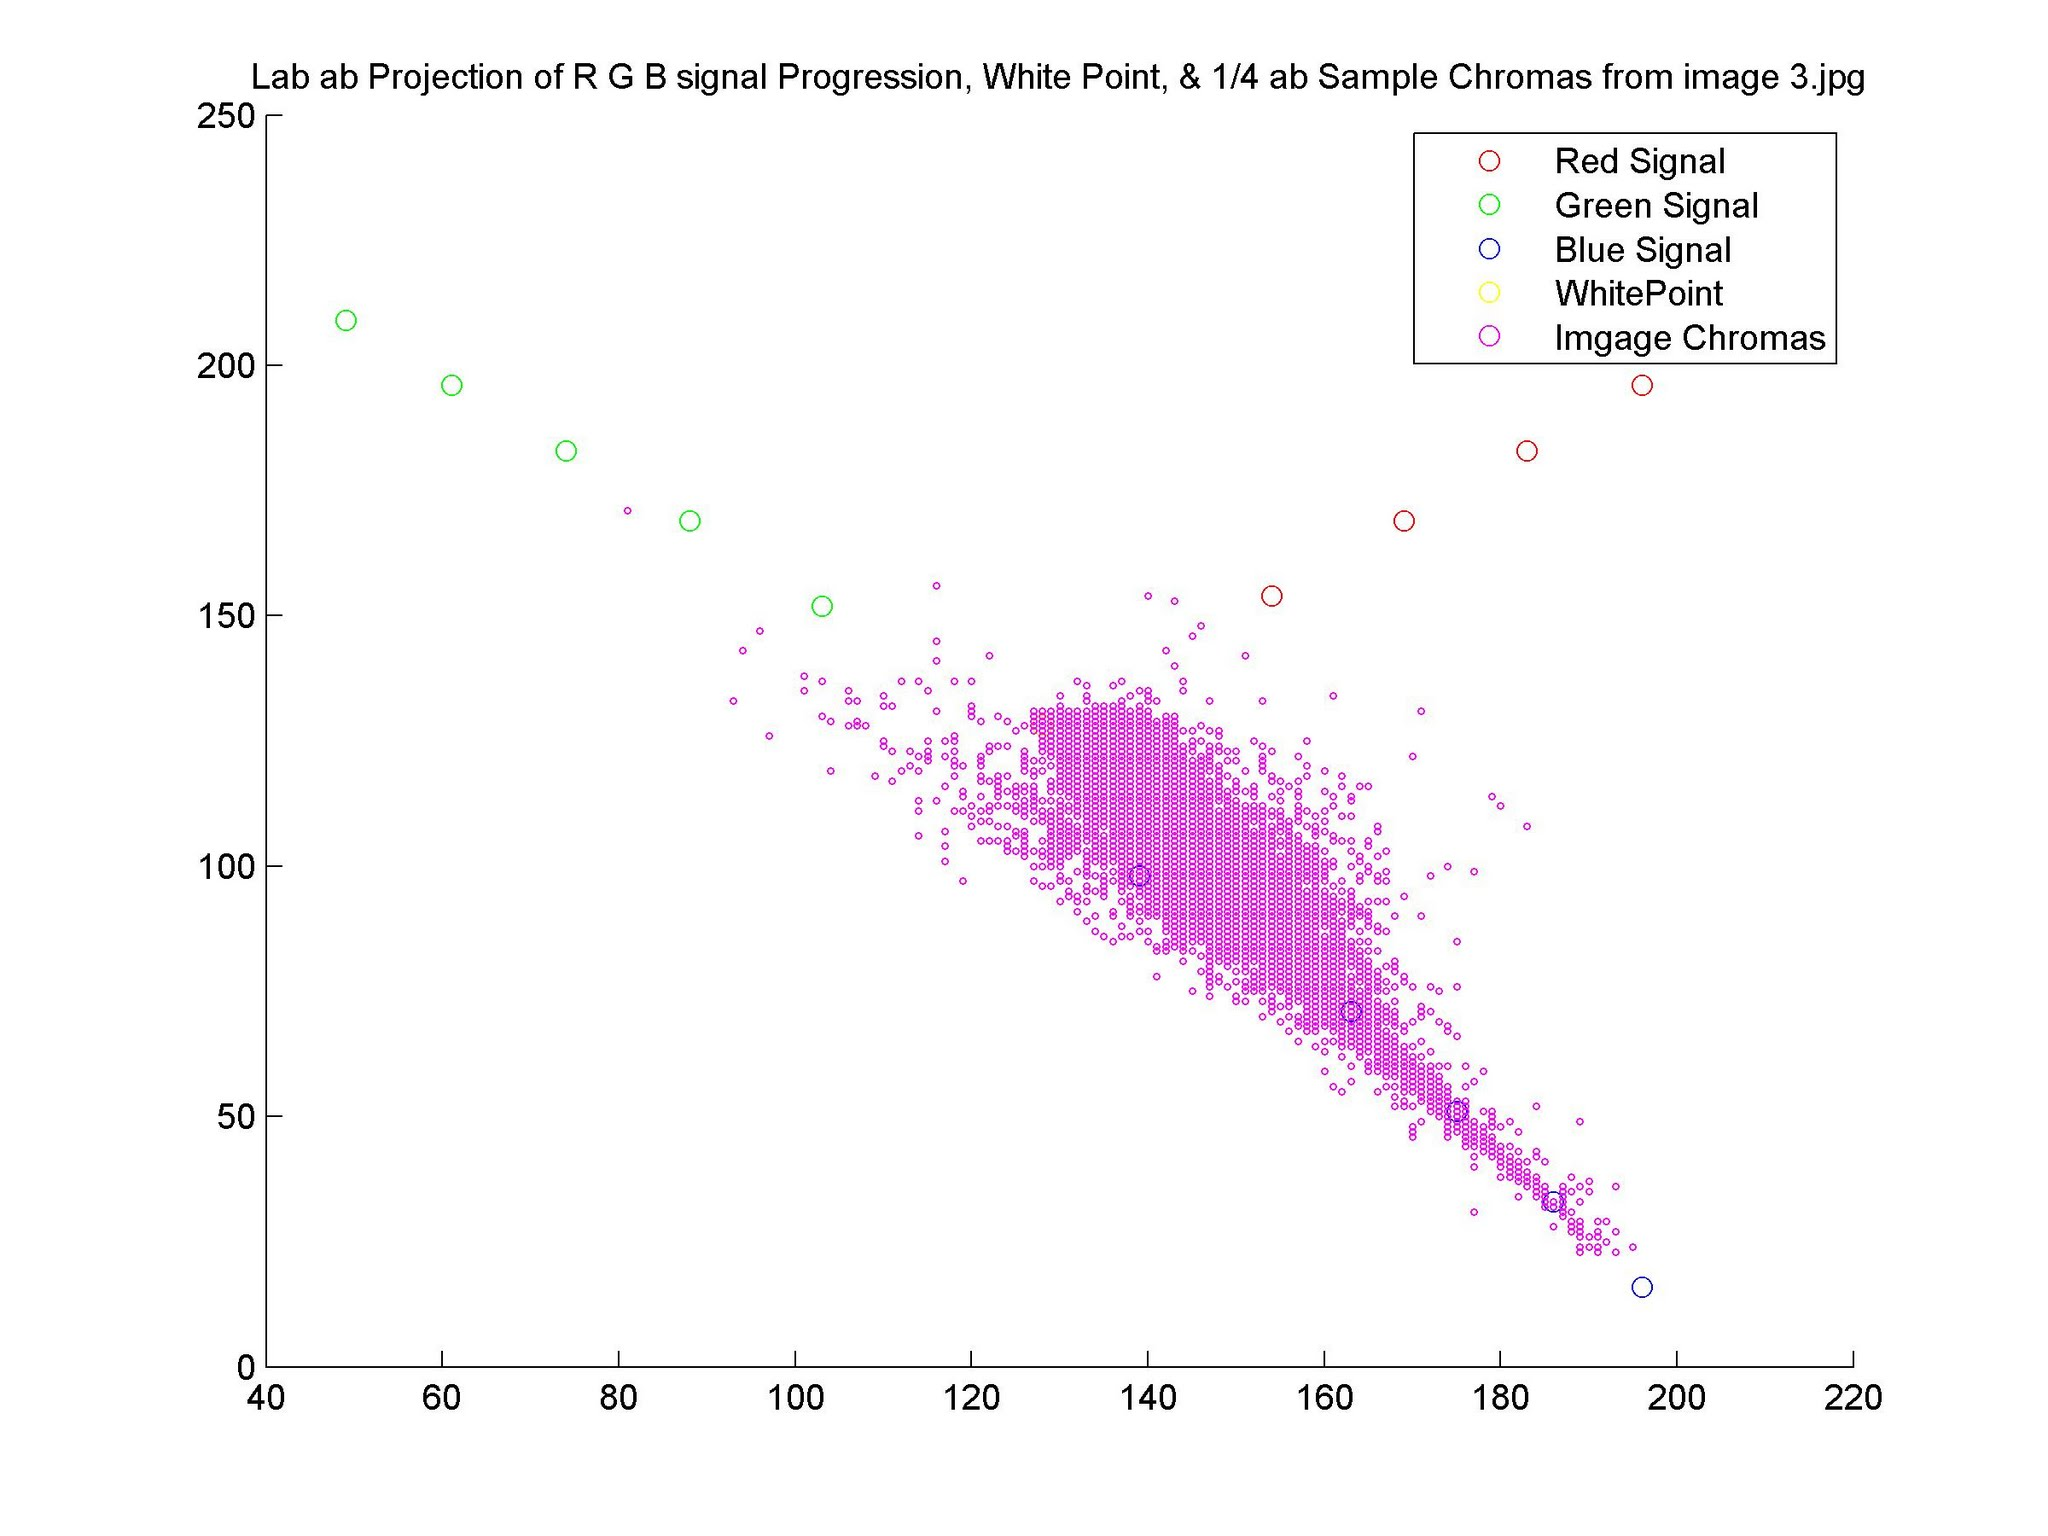
\includegraphics[width=5.0cm,height=5.0cm]{images/Her2Fish/3_SampleChromas.jpg}  \\
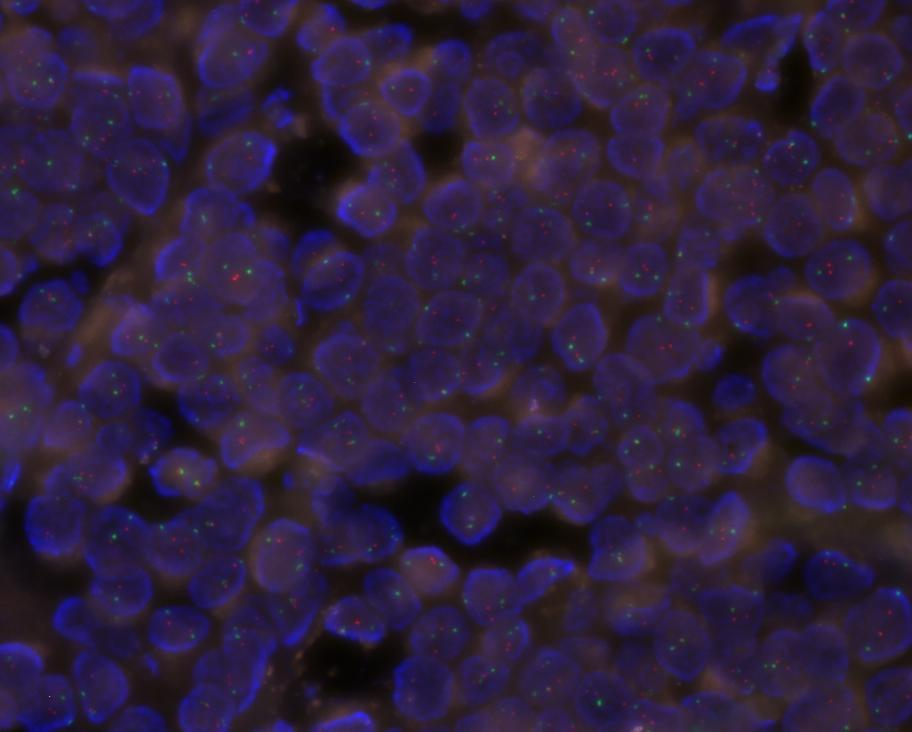
\includegraphics[width=5.0cm,height=5.0cm]{images/Her2Fish/4.jpg}               &
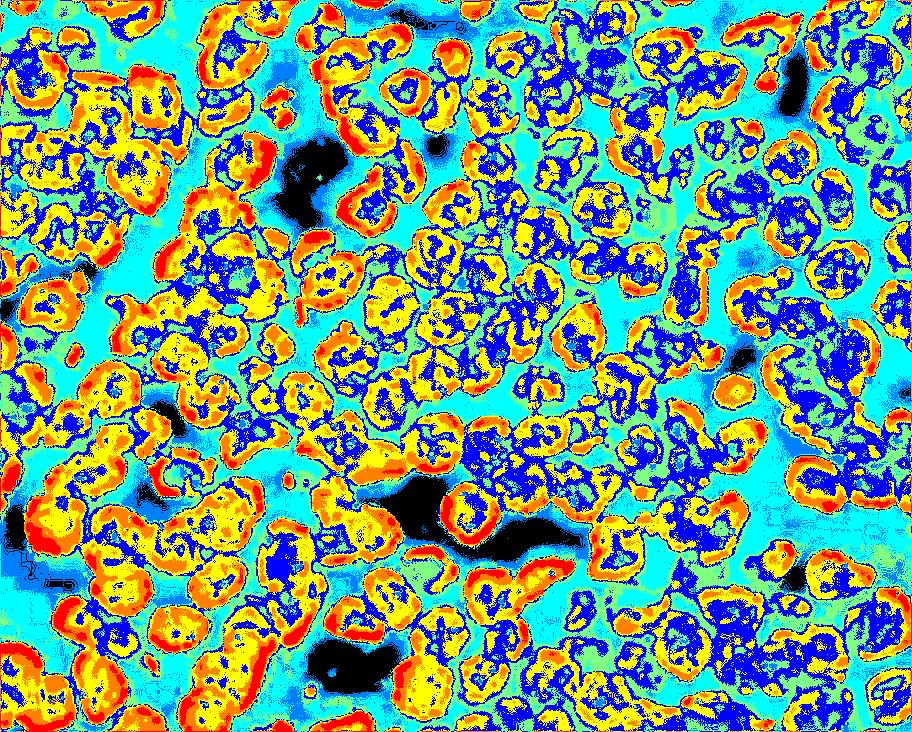
\includegraphics[width=5.0cm,height=5.0cm]{images/Her2Fish/4_RGB_LabelImg.jpg}  &
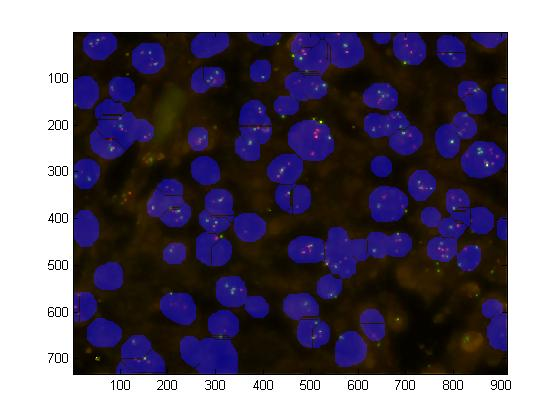
\includegraphics[width=5.0cm,height=5.0cm]{images/Her2Fish/B31-1677A108_ProcessedlabelimageWithSpotsEnhanced.jpg}  \\
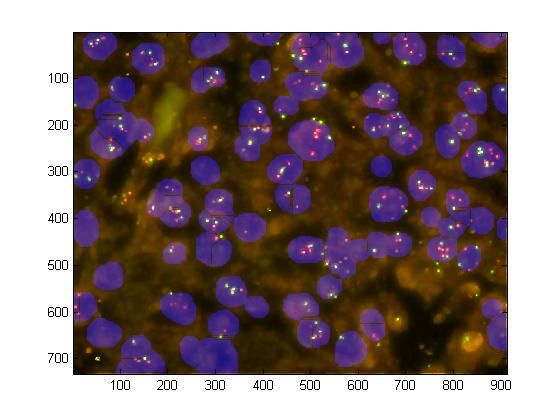
\includegraphics[width=5.0cm,height=5.0cm]{images/Her2Fish/B31-1677A108_ProcessedlabelimageWithSpotsEnhanced2.jpg}  &
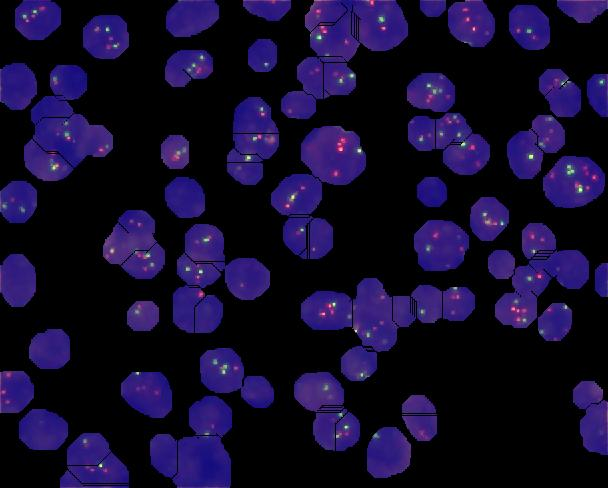
\includegraphics[width=5.0cm,height=5.0cm]{images/Her2Fish/B31-1677A108_ProcessedlabelimageWithSpotsEnhanced3.jpg}
\end{tabular}

\subsection{Development of a commercial system for automated HER-2/CEP17 FISH analysis}
A cost benefit study of Her2 assessment at the McGill University Health Center reports\cite{HER2FISH1}:
\emph{"If all women with newly diagnosed breast cancer were screened with fluorescence in situ hybridization, the cost of testing would be increased by about \$303 000 for every 1000 women screened (compared with Strategy 1); however, the percentage of accurate diagnoses would be expected to be 100\%"}
There is considerable benefit to be obtained by bringing the cost of Her2 FISH analysis down. A commercial machine vision system for analysis would help accomplish that. An initial milestone would be a research quality software implementation to demonstrate the feasibility of a commercial implementation.
Our initial results indicate that a research quality implementation is possible with a modest amount of effort. The cost will involve machine vision development time and pathologist time for the capture of classifier training data and evaluating system performance. Image capture is not considered at this time. Some options are available:
\begin{itemize}	
\item A microscope based CCD microscopy camera coupled with servo controlled stages.
\item 	Modify the optics of a whole slide scanner to capture the images under the correct illumination for FISH analysis.
\end{itemize}

\section{Segmenting HES Skin}
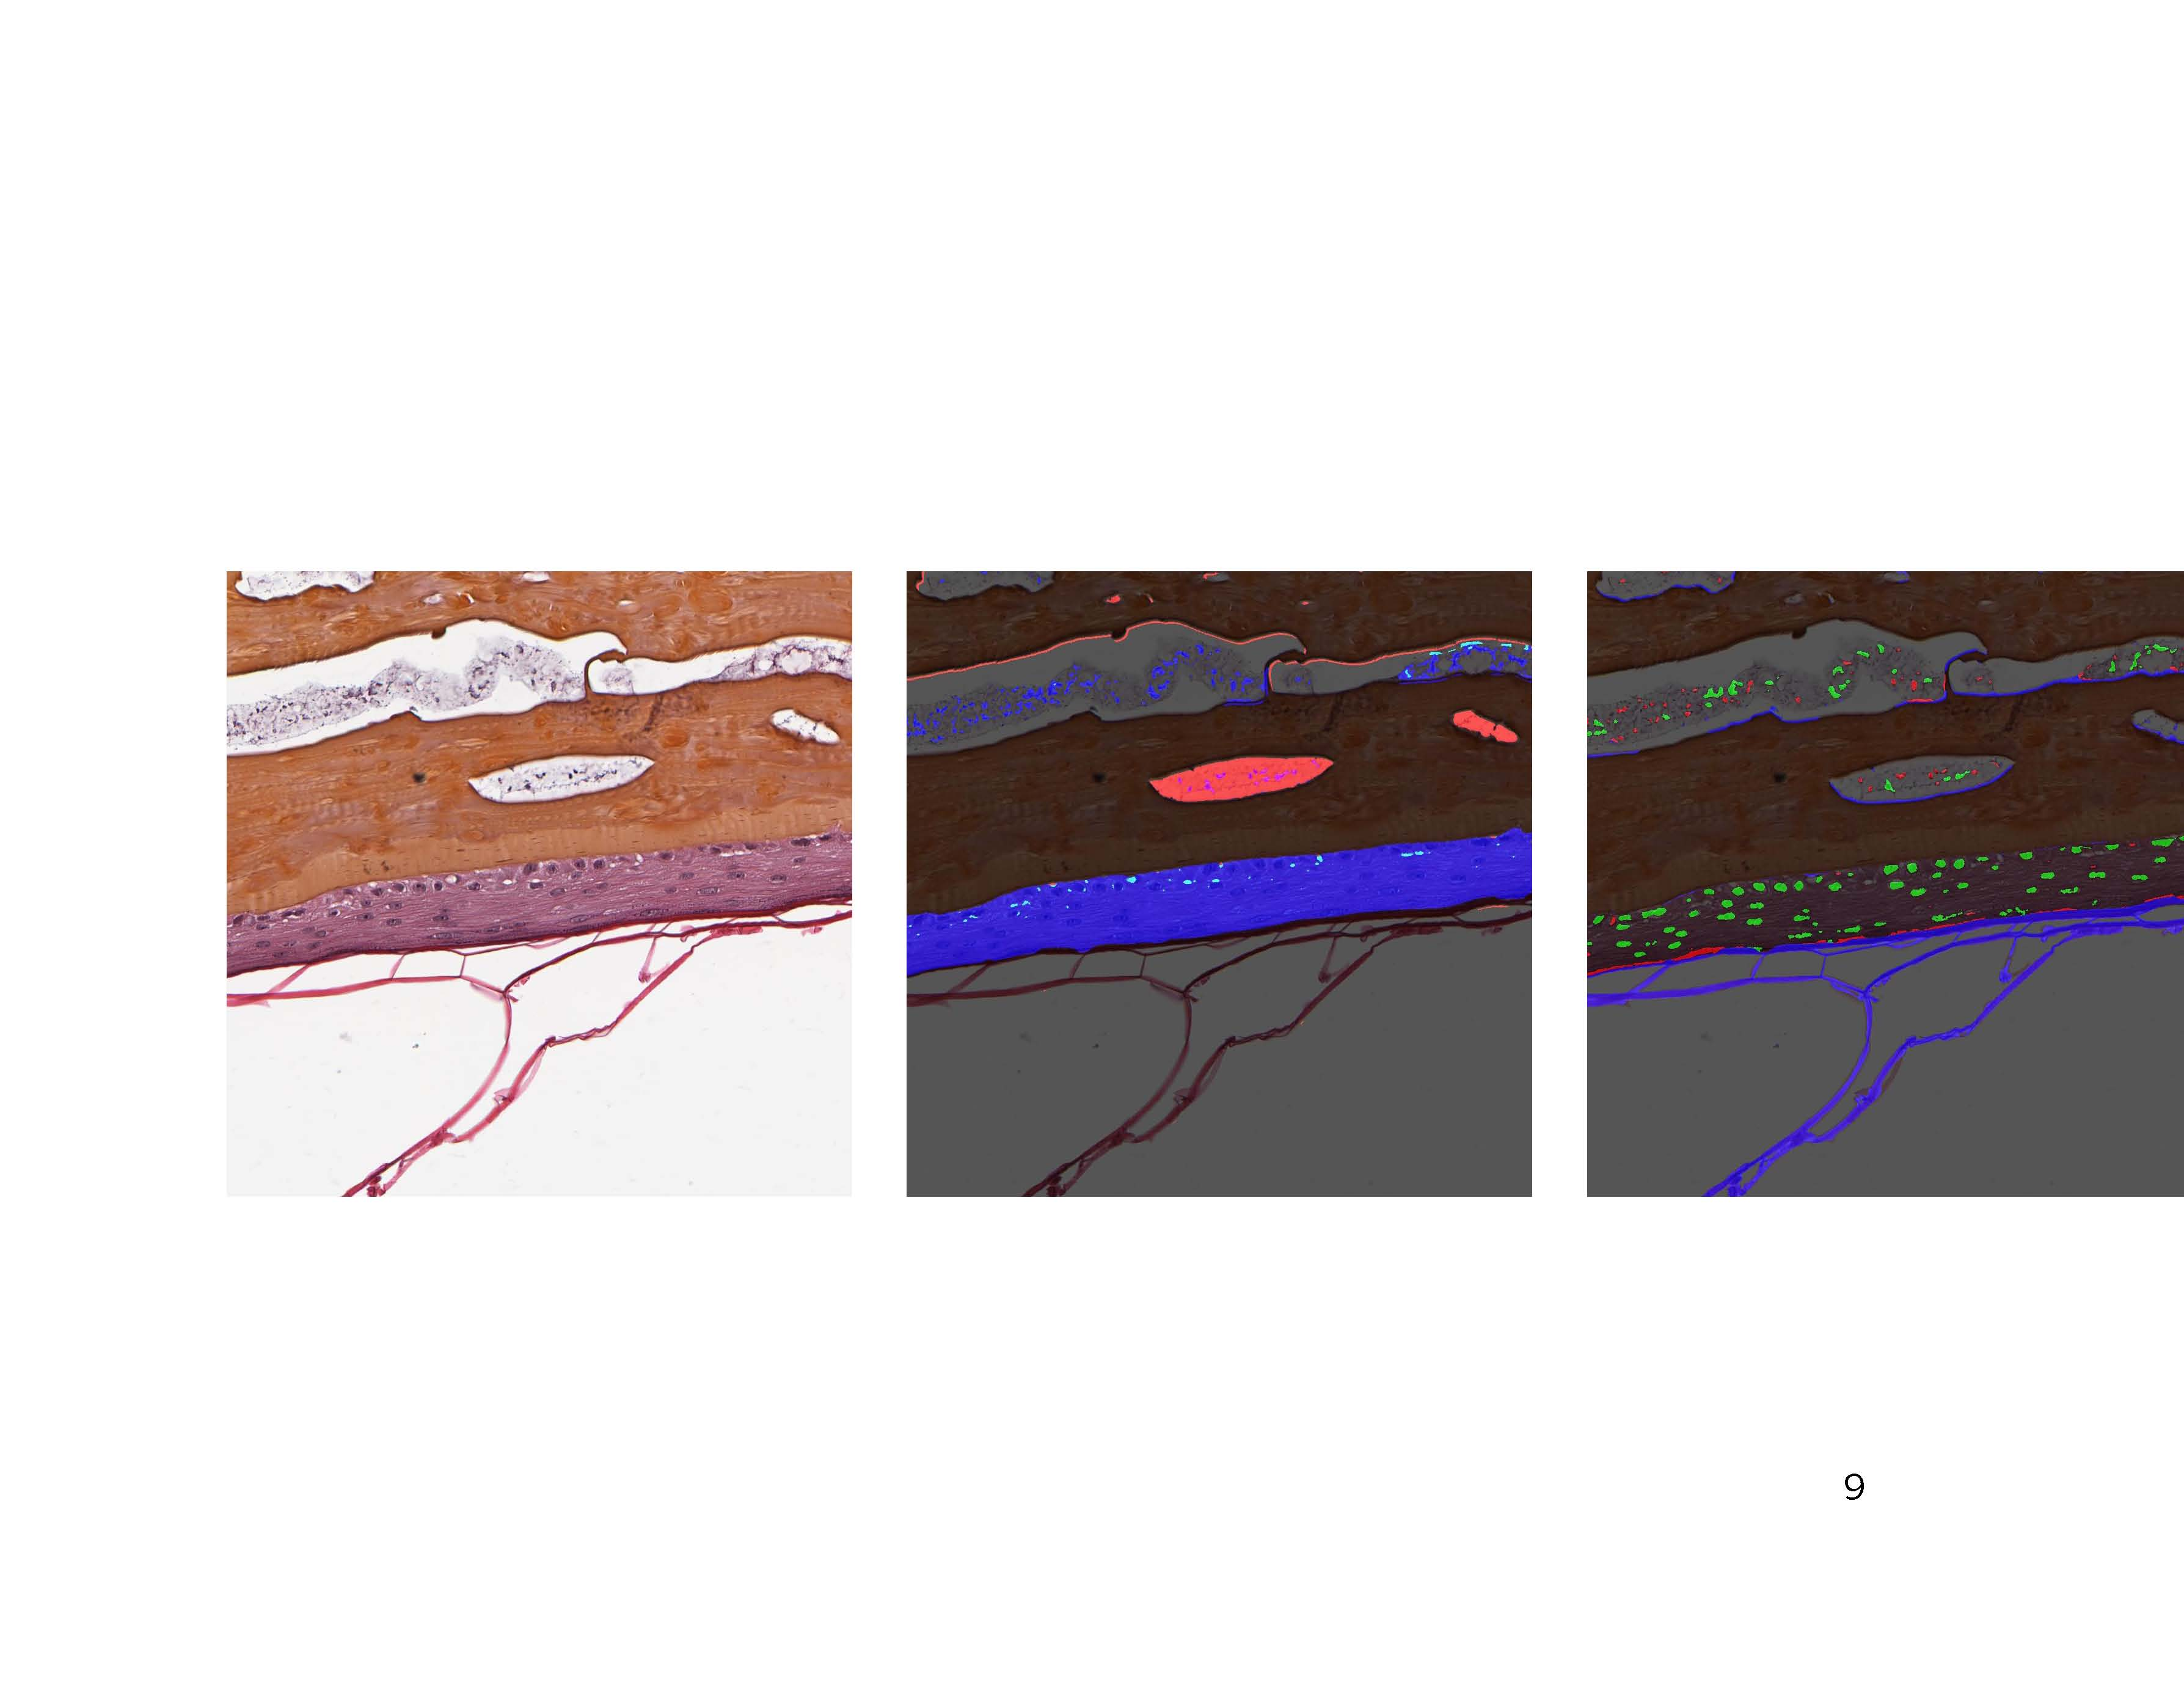
\includegraphics[width=8.0cm,height=8.0cm]{images/MachineVision/MachineVision_Pathology_ExampleSlides_Page_11.jpg}

\section{Segmenting in Lab chromaticity or PCA space using k-means clustering}
Automatic segmentation using the convex hull of chromaticity space to seed k-means. This or a PCA on optical density space form the basis of object feature development. PCA is more appropriate when the stain is known. Following are dermis images from http://tray.dermatology.uiowa.edu.

\includegraphics[width=8.0cm,height=8.0cm]{images/MachineVision/MachineVision_Pathology_ExampleSlides_Page_13.jpg}

\bibliographystyle{amsplain}
%
%\bibliography{MVbib}
%\end{document}
% -------------

%\end{document}
% ----------------------------------------------------------------


